\documentclass[12pt]{extbook}
%\usepackage[fontsize=12pt]{fontsize}
\usepackage{fancyhdr}
\usepackage{graphicx}
\usepackage{bm}
\usepackage[fleqn]{amsmath}
\usepackage{amsfonts}
\usepackage{amssymb}
\usepackage{amsbsy}
\usepackage{wasysym}
\usepackage{subfigure}
\usepackage{multirow}
%\usepackage{txfonts}
\usepackage{float}
\usepackage{color}
\usepackage{textcomp}
\usepackage{caption}
\usepackage{ragged2e}
\usepackage{longtable}
\usepackage{nameref}

\linespread{1.2}
%\setlength\parskip{0.5\baselineskip}
\pagestyle{fancy}
\fancyhf{}% Clear header/footer
\fancyhead[LE]{{\it \rightmark}}
\fancyfoot[LE]{{\it \thepage}}
\fancyhead[RO]{{\it \rightmark}}
\fancyfoot[RO]{{\it\thepage}}
\renewcommand{\headrulewidth}{0.4pt}% Default \headrulewidth is 0.4pt
%\renewcommand{\footrulewidth}{0.4pt}% Default \footrulewidth is 0pt


\begin{document}

%====================================END OF DEFINITION =============================
\pagenumbering{Roman}
\centering
Abstract of thesis entitled\\
~\\
{\Large \bf Integrated optimization design framework for metallic orthopedic devices with graded-density lattice microstructures}\\
~\\
submitted by\\
~\\
{\Large \bf Jiuzhao Zhou}\\
~\\
for the degree of Doctor of Philosophy\\
at the University of Hong Kong\\
in November 2022\\
~\\
\justifying
Porous femoral implants and spinal cages have drawn increasing attention in the treatment of total hip arthroplasty and lumber inter-body fusion for their satisfactory performance in ossature bio-mimicity. Nevertheless, conventional porous orthopedic devices adopt uniform-density and isotropic lattice microstructures, which does not accord with the actual loading condition in femur and spine. In this thesis, an integrated optimization design framework is proposed for metallic femoral implants and spinal cages with graded-density and anisotropic lattice microstructures. The framework includes three moduli: lattice microstructure mechanical property homogenization, gradient-based device topology optimization and lattice device configuration reconstruction.\\

As a pre-request of optimization design, a data-driven mechanical property homogenization system for anisotropic lattice unit cells is established based on Gaussian process (GP) machine learning model. Key parameters of the GP kernel is fitted by training a pre-prepared sample dataset. The system can promptly predict stiffness modulus and failure strengths of simple orthotropic lattice unit cells with arbitrary interior architecture. The reliability of GP homogenization system is verified by error and correlation analysis on testing dataset. Results reveals that single-output GP process achieves highest prediction accuracy than multi-output GP process. The maximum prediction error observed is lower than 10\%. Strong positive correlation close to 1 is observed on GP-predicted output variables and their reference values.\\

Optimization designs are conducted for anisotropic lattice femoral implant and isotropic graded-density lattice spinal cage. Maximum global compliance in orthopedic device is selected as the objective function of optimization framework. Metallic materials are moved from high-stress zones to low-stress zones in devices, so that the locally-concentrated bone stress is re-allocated to areas with lower stress, which moderates the stress shielding problem in femur and vertebrae. Constraint conditions of the optimization are designed based on clinical requirements and additive manufacturing capabilities. The design of femoral implants and spinal cages utilizes MMA algorithm. Four loading conditions with different body load eccentricity are simulated for design of spinal cage. The bio-mechanical performance of the optimized devices are evaluated by calculation of resorbed bone mass fraction and global stress shielding intensity. After optimization, the graded-density anisotropic femoral implant successfully reduces the resorbed bone mass fraction by 39.4\% and 47.5\% compared to graded-density isotropic and uniform-density cases. For spinal cage, reduction of resorbed bone mass fraction by 17\% to 38\% is achieved by the MMA algorithm.\\

Upon the completion of optimization domain, in order to convert the optimal design variables to printable lattice device configurations, a series of reconstruction instructions are proposed for orthopedic devices meshed with different types of elements. The configuration of optimized anisotropic femoral implant and graded-density spinal cages are presented, based on which the device product for clinical use can be directly fabricated via additive manufacturing technique.\\

(451 words)\\
\newpage
\thispagestyle{empty}
~\\
%=============================================================================
\newpage
\thispagestyle{empty}
\centering

{\Large \bf Integrated optimization design framework for metallic orthopedic devices with graded-density lattice microstructures}\\
~\\
~\\
\begin{figure}[htbp]
\centering

\includegraphics[width=5 cm]{fig/logo}
\label{e_error}
\end{figure}
~\\
{\bf \large Jiuzhou Zhao}\\
~\\
Department of Civil Engineering\\
The University of Hong Kong\\
~\\
Thesis submitted to the University of Hong Kong,\\
in partial fulfillment of the requirements for\\
the degree of Doctor of Philosophy.\\
~\\
~\\
November 2022\\

\justifying

\newpage
\thispagestyle{empty}
~\\
%=============================================================================
\newpage
\thispagestyle{empty}
\centering
{\bf \large Declaration}\\
~\\
\justifying
I hereby declare that the thesis entitled ``Integrated optimization design framework for metallic orthopedic devices with graded-density lattice microstructures'' represents my own work, except where due acknowledgement is made, and that it has not been previously included in a thesis, dissertation or report submitted to this University or to any other institution for a degree, diploma or other qualifications.\\

\flushright

Jiuzhou Zhao\\
November 2022\\

\justifying
\newpage
\thispagestyle{empty}
~\\

%=============================================================================
\newpage
\thispagestyle{empty}
\centering
{\bf \large Acknowledgement}\\
~\\
\justifying
First and foremost, I would like to devote my deepest gratitude to my supervisor, Professor Xiaowei Deng, for his guidance and encouragement throughout my research. Professor Deng can always identify cutting-edge research topics and shares with us. He can always point out the weakness of my research work and explore solutions with me. I would also like to thank my co-supervisor, Professor Ray Kai Leung Su. He brought me to the world of finite element analysis. I would like to express my sincere thanks to Professor Grace Teng Zhang. She always provides me sufficient support when I am faced with challenges from medical research field.\\

I would like to thank my labmates: Jiajun Chen, Zhikun Dong, Xinxin Feng, Senbin Huang, Mahram Khan, Chermila Piyumi, Qiulei Wang, Kun Yang, Shanghui Yang. I will never forget those days we stayed together,\\

I would like to thank the department's general office staff for helping me with my research life. They are very responsive, kind, professional, and helpful.\\

I deeply appreciate my parents, Shufu Zhao and Yanxia Sun, my other relatives, and all of my friends for their all-round support. I would like to show special thanks to my close friend Zhuoran Ji, for his selfless technical supports on my research work.\\

Finally, I would like to express my deepest and most sincere apologies to my grandmother and grandfather's mother. They passed away during my doctoral research days. Every time I left my hometown for Hong Kong, I told them I would be back soon, like in a few months. But every time I broke my promise.\\
\thispagestyle{empty}
%=============================================================================
\newpage
\setcounter{page}{1}
\pagenumbering{roman}

\tableofcontents

\newpage

\listoffigures

\newpage

\listoftables

\newpage
\thispagestyle{empty}
~\\

%=============================================================================
\newpage
\setcounter{page}{1}
\pagenumbering{arabic}

\chapter{Introduction}
\label{intro}

\section{Background}
\label{intro_back}

In orthopedic clinical treatment, metallic devices are commonly utilized to achieve desired bio-mechanical functions in patients's skeleton system. Among different replacement treatment techniques, total arthroplasty replacement and lumbar inter-body fusion attract special attentions for their treatment efficacy in hip joint disability and low back pain. During the operation process, metallic femoral implant and spinal cages are implanted to act as load-bearing component of human body.\\

\subsection{Hip joint disability}

Hip joint disability (HJD) is a common health threat in modern society. Its main causes are generally arthritis-attributed, including osteoarthritis, rheumatoid arthritis and the traumatic arthritis~\cite{foran2015total}. HJD seriously affects the walking and standing capability of patients, causing additional cost of treatment. During 2010 to 2012, the prevalence of arthritis was 52.5 million and the prevalence of arthritis-attributable activity limitation is 22.7 million in US~\cite{barbour2013prevalence}. These two indices are predicted to be 78.4 million and 34.6 million in 2040~\cite{hootman2016updated}.\\

\subsection{Total Arthroplasty Replacement}

Top hip arthroplasty (THA), also termed as total hip replacement, is a widely adopted surgical treatment method for patient with severe hip joint disability. The first step of the treatment process is to remove the diseased femur head and cancellous bone tissue inside the femur neck. An artificial femur implant is then inserted into the femur neck as a replacement of femur head, acting as the load bearing structure between femur shaft and pelvis. Femur implant for THA treatment is usually made of the pure titanium alloy. Among common commercial materials used for medical devices, titanium has the best bio-compatability, which stimulates the bone growth after surgery~\cite{olivares2015implant}. THA is now widely accepted by HJD patients. In year 2014 and 2018, the number of THA clinical application cases performed in Canada raised from 49,819 to 58,492, indicating a 17.4\% increment~\cite{canadian2019hip}.\\

Nevertheless, THA is meanwhile criticized for its high revision surgery rate. During 1979 to 1998, 20\% of 10,000 Norway THA patients were required to take revision surgery within one year after THA surgery~\cite{malchau2000update}. In 2018, the revision surgery rate in Canada is 8.2\%, implying 4,822 revision treatment and \$89 million extra inpatient cost on healthcare system~\cite{canadian2019hip}. The major cause for THA failure is aseptic loosening, occupying a 75.7\% share in Norway during 1979 to 1998~\cite{malchau2000update}.\\

Studies reveal that the loosening of implant results from stiffness incompatibility between titanium alloy and femur bone tissue. The stiffness of Ti$_6$Al$_4$V (approx. 119 GPa~\cite{bandyopadhyay2010influence}) is nine times higher than the stiffness of cortical bone (approx. 12 GPa~\cite{wirtz2000critical}). The femur implant with stronger stiffness concentrates more body loading, leading to reduce stress in femur bone tissue surrounding the implant. According to Wolff's law, stress in bone tissue acts as bone growth stimuli~\cite{wolff1893gesetz}. As a consequence, the deterioration risk at femur neck and shaft increases after THA treatment. Currently, stress shielding has been regarded as an important cause to postoperative femur bone degeneration~\cite{head1995titanium}.\\

\subsection{Low back pain}

Low back pain (LBP) is a common health threat in modern society. In 2000, its wold-wide life time prevalence is estimated to be 38.9\%~\cite{hoy2012systematic}. In developed countries with large amount of aging population, this number can be 60\% to 80\%~\cite{vos2012years}. Statistics show that the annual prevalence of LBP is significantly higher in women (35.3\%) than in men (29.4\%)~\cite{hoy2012systematic}, while high-income individuals (32.9\%) are more likely to suffer from the disease than middle-income (25.0\%) and low-income individuals (16.7\%)~\cite{hoy2012systematic}. Notably, intractable LBP demonstrates a strong age correlation. As shown in Figure 1, the 60-to-69-year-old age group was most likely to suffer from LBP ~\cite{hoy2012systematic}. Overall, middle-aged and older adults (30 to 89 years) have a higher risk of developing the condition than adolescents (10 to 29 years)~\cite{hoy2012systematic}~\cite{taimela1997prevalence}~\cite{manchikanti2009comprehensive}.\\

Currently, the vast majority of intractable LBP is triggered by abnormalities in the lumbar discs. Data show that 39\% of cases are non-displaced discogenic LBP, which is the major cause of this disease. Another 30\% of LBP cases was caused by lumbar disc herniation~\cite{grabovac2019association}. Other non-mainstream causes include lumbar foraminal stenosis, lumbar degenerative instability, lumbar degenerative dislocation, lumbar degenerative scoliosis, and small joint syndrome, etc~\cite{makris2017physical}.\\

For patients, persistent LBP poses a long-term physical, psychological, and financial burden. About 17\% LBP patients lose their working ability~\cite{hoy2012systematic}. Some patients cannot complete daily activities such as stairs-climbing and clothing~\cite{casazza2012diagnosis}. A significant number of patients are alienated from family, friends, and society due to mobility problems, which resulting to negative emotions~\cite{kim2019expenditures}. More than 31\% of patients undergo continuous treatment for six months before the the complete elimination of back discomfort, but between 25\% and 62\% of patients have a relapse within two years~\cite{pinheiro2015advanced}. At the societal level, the large population of patients with lower back pain adds loads to the health care system and causes financial losses. In the United States, according to statistics for the decade 2007-2016, the average patient spent \$676 (without surgery) or \$17,640 (with surgery) for treatment within one year after diagnosis~\cite{wolfe1995prevalence}. The nation-level total cost is \$2.1 billion~\cite{wolfe1995prevalence}. Also, the loss of work productivity due to the inability of adult patients should be regarded as another economic loss~\cite{guo1999back}. This loss in UK and US are 100 million~\cite{zhang2009clinical} and 150 million~\cite{herkowitz2011rothman} capita working days respectively.

\subsection{Lumbar interbody fusion}

As a popular treatment method, lumbar interbody fusion (LIF) retains the load bearing ability of necrotic functional spine unit (FSU). Firstly, the degenerated intervertebral disc is removed and the vertebra endplates are polished. Afterwards, a spinal cage is placed between vertebrae. It transfers loading through the spine and stimulates bone tissue at endplate surfaces. In long term, the two vertebrae merge and no relative displacement between them happens, so as to avoid potential neurothlipsis on cord~\cite{mobbs2015lumbar}~\cite{yavin2017lumbar}.\\

LIF can be further classified into anterior approach fusion, posterior approach fusion, transforaminal approach fusion, and extreme lateral approach fusion [16]. Among these categories, transforaminal approach fusion can avoid most of the organs, muscles and nerves in the surgical path~\cite{mobbs2015lumbar}. Compared with the posterior approach fusion, it has a better clinical performance because it causes less damage to the spinous and transverse structures and is preferred by the treating patients~\cite{mobbs2015lumbar}. Compared to conservative treatment methods, LIF shortens the length of hospital stay~\cite{mobbs2015lumbar}. In the United States, from 2000 to 2009, the number of fusions performed per million people doubled from 75 to 178, reflecting its enhancing market acceptance, despite an increase in average cost from \$25,000 to \$82,000~\cite{yavin2017lumbar}.\\

Conventional spinal cage fully made of metallic material is criticized for its high failure risk. More than 20\% of LBP patients undergo at least one revision surgery within eight years since their primary LIF surgery~\cite{abdu2018long}. The main cause of revision surgery is the stiffness incompatibility between bone tissue and cage. Most orthopedic devices are manufactured with stiff metallic materials such as Ti$_6$Al$_4$V (approx. 119 GPa), cobalt-chromium alloy (approx. 53 GPa) and stainless steel (approx. 51 GPa), which are much stiffer than both cortical bone (approx. 15 GPa) and cancellous bone (approx. 4 GPa)~\cite{warburton2020biomaterials}. Different to rubber-like spinal disc, metallic cages with low deformation flexibility can hardly redistribute reaction force among endplate surfaces. Besides, the pre-designed cage interior structure is not customized for the actual physique condition of individual patients, which further contributes to the stress variation in post-operative lumbar vertebrae~\cite{reid2019state}~\cite{jain2016advances}. According to Wolff's law, lack of stress stimuli leads to bone tissue degeneration~\cite{wolff1893gesetz}. The unexpected stress reduction in vertebrae can cause adverse events including pseudarthrosis, segment degeneration and implant failure~\cite{williams2005ct}~\cite{pimenta2012biomechanics}~\cite{pichelmann2010revision}.\\

\subsection{Lattice structures}

As a representative meta-material, porous structures refer to artificial materials with self-compacting interior structures and exhibit mechanical properties unavailable in nature. Porous materials include two categories: cellular materials and lattice materials. Foam materials (Figure 4a) contain randomly arranged closed cavity units. Compared with conventional materials, foams show outstanding capability in kinetic energy absorption and thermal isolation~\cite{elmarakbi2013advanced} and are therefore widely used in the production of automotive/marine buffers and in the interior filling of building structures~\cite{mazur2017mechanical}. Currently, most of the foams are manufactured by chemical bubbling or soluble aggregates~\cite{fleck2004overview}, which is cost-competitive but do not allow precise control of the mechanical property distribution at the macroscopic level.\\

Different to cellular materials, lattice materials (Figure 4b and Figure 4c) are designed with aspiration from the arrangement of atoms in the crystal. At the microscopic scale, they often exhibit a short beam or truss-like configuration, while the cavities inside the cells are connected to each other and to the outside. By controlling the microstructure and porosity, designers can achieve their desired mechanical properties (stiffness / Poisson's ratio, etc.) in macroscopic level. Besides, the graded-density characteristic of lattice material allows the application of other meta-material design concepts, such as stretchable origami structures, to provide controlled large deformation capabilities~\cite{bobbert2018towards}. Nowadays, great progress has been made in the bistable design~\cite{jianguo2014morphology}~\cite{jianguo2015bistable} and foldable analysis~\cite{cai2016deployment}~\cite{cai2016motion}~\cite{cai2017deployment} of origami materials.\\

\subsection{Additive manufacturing}

Traditional industrial manufacturing techniques (e.g. casting, forging) require fixed product design. Temporary configuration adjustments could be expensive. As an advanced high-precision manufacturing technology, additive manufacturing (AM) provides higher flexibility for the design and manufacture of industrial products. Generally, AM builds products by printing material particles layer by layer with micrometer accuracy~\cite{calignano2017overview}. The entire manufacturing process is highly automated, enabling direct transition from 3D model configuration design files to final products. This characteristic makes AM particularly suitable for the low-cost rapid mass fabrication of structural products with complex~\cite{mahmoud2017lattice} and customized configurations~\cite{gupta2015recent}. Currently, AM has been widely used in aerospace and mechanical~\cite{liu2017aerospace}\\

\section{Motivations}
\label{intro_moti}

\subsection{Lattice microstructures and orthopedic devices}

Lattice structures provide higher design flexibility to medical devices. By controlling strut configurations (i.e. thickness, position), mechanical properties of the lattice cell can be adjusted without change of basis material. Multiple studies verify the positive effect of lattice orthopedic devices on bone growth stimulation and stress shielding mitigation.\\

Via fluorescence technique, the bone growth rate can be directly quantified in animal experiments. Results show that despite of configuration of lattice microstructures (e.g. triangle, hexagonal, rectangular), bone growth rate is positively related to implant local porosity~\cite{cheng2014additively}~\cite{van2012effect}~\cite{li2007bone}. On the one hand, porous microstructures mimic the real bone internal environment (70-90\% porosity) and helps stimulate skeletal cell division and differentiation~\cite{balla2010porous}. Besides, higher porosity results in rougher implant surfaces, enhancing friction on the implant-bone interface in the immediate postoperative period and hence preventing the implant dislocation after implantation~\cite{xue2007processing}. Finally, larger implant surface porosity means larger space inside implant domain, which provides sufficient space for cell ingrowth and attachment.\\

Tracking record of human total hip replacement clinical cases shows that higher implant porosity sufficiently moderates severity of stress shielding in femur bone~\cite{khanoki2013fatigue}~\cite{arabnejad2012multiscale}~\cite{wang2018hip}~\cite{arabnejad2017fully}. Different to fulfilled solid implants, implants with lattice interior structures can transfer bone-implant interface pressure from high-pressure zones to low-pressure zones, so that to achieve a more uniform stress distribution in femur head and shaft~\cite{wang2018hip}~\cite{arabnejad2017fully}.\\

\subsection{Optimization design and orthopedic devices}

Integrated with finite element analysis method, topology optimization (TO) design has been widely applied in precious design of stress bearing structures. In building structure design field, SIMP algorithm is used to re-allocate the material distribution in tubular joint so as to avoid stress concentration nearby welding points~\cite{huang2021integrated}.\\

In femoral implant design field, parameterized level set method (LSM) was used to customize the structure of total femur prosthesis~\cite{deng2015topology}. The modified LSM with Boolean R-function not only achieved enhanced prosthesis stiffness with lower material usage, but also took the cartilage surface wear and erosion as optimization consideration. Similar optimization method has been practiced in femur implant design. Niroomand and Boroomand applied SIMP to simplify femur and implant model. By changing the shape of the implant, they achieved more uniformly distributed von Mises stress in the optimization domain with 16\% reduction in material consumption~\cite{niroomand2018application}. With the same volume fraction reduction, Munteanu et al. further reduced the maximum stress in implant by 27\% and showed the feasibility of additive manufacturing of the optimized implant sample~\cite{munteanu2019additively}.\\

By adopting lattice microstructures in femoral implant, the optimization design efficiency is further enhanced. By controlling lattice strut thickness, local mechanical property can be adjusted without change of material. As a proof-of-concept research, Arabnejad and Pasini in 2012 conducted multi-scale and multi-objective optimization design on 2D graded-density titanium hip implant using NSGA-II algorithm~\cite{khanoki2012multiscale}. The optimized graded-density implant reduced 45\% resorbed bone mass and 23\% maximum interface failure index compared to uniform-density implant. This design concept is then extended to 3D hip implants~\cite{arabnejad2017fully}~\cite{wang2018hip}. Besides relatively density, unit cell morphology also affects implantation performance. In 2016, Arabnejad et al. fabricated eight titanium alloy unit cell samples in four different relative density and two cell morphologies~\cite{arabnejad2016high}. Compression tests and animal (canine) experiments show differentiated against both design variables.\\

The concepts of finite element simulation and topology optimization have also been applied to the design of intervertebral fusion devices. In earlier studies, the configuration~\cite{zhong2006finite} and wall thickness~\cite{schnitzer2020comparison} of the cage are optimized to save material usage, enhance spinal stability and moderate stress shielding. Cage samples are additive manufactured via selective laser melting method using Ti$_6$Al$_4$V basis material for verification experiments~\cite{schnitzer2020comparison}. Bashkuev in 2015 introduced lattice microstructure in cage design and used mechano-regulation algorithm to evaluate its influence on bone growth stimulation, providing precious reference information on cage surface porosity control~\cite{bashkuev2015computational}. Chen in 2021 evaluated the biomechanical responses of PEEK cage with different global porosities, revealing that increment in porosity reduces endplate surface pressure and avoids cage subsidence and migration~\cite{chen2021computational}. In the same year, Pan further proposed the design idea of partitioned spinal cage~\cite{pan2021design}. His team divided the cage into multiple parts with different relative densities, thereby controlling the local stiffness of the fusion device more precisely and making it more similar to the mechanical characteristics of human bone.\\

\subsection{Current shortcomings}

Albeit lattice orthopedic devices have been utilized in clinical treatment, in current stage, there are still significant deficiencies in their interior configuration design.\\

\begin{enumerate}

\item {\bf The versatility of microstructure configuration is limited.} Most of current studies only focus on the relative density variation of isotropic lattice unit cells and the resulting change in mechanical properties. The influence of microstructure architecture itself is rarely discussed. As one of the only few examples, Xu et al. created anisotropic lattice unit cells by adjustment of material allocation on unit cell structs on different directions~\cite{xu2016design}, making it feasible to assemble vertically strengthened femur implant to match the actual stiffness condition in femur bone~\cite{painkra2018anisotropic}. However, the real-time computation of anisotropic lattice unit cell mechanical property is time-consuming with common homogenization methods~\cite{dong2019149}. Some analytical mechanical property models are proposed but are only applicable to certain cell configurations~\cite{xu2016design}. Therefore, an universal mechanical property prediction model for different lattice unit cell structures is desired.\\

\item {\bf Optimization design methodologies for orthopedic devices, especially for spine fusion devices, lack for exploration.} Most existing studies do not discuss the correlation between target functions and stress shielding severity, making the algorithm difficult to make accurate response to the actual stress condition inside critical bone tissues and finally dragging down the efficiency of optimization design. Considering the 
significant differences between patient physiques, in-depth discussion should be made on optimization algorithm design against different medical case scenario (e.g. THA / LIF) and physique conditions (e.g. hunchback / spinal scoliosis)~\cite{ezquerro2004combination}.\\

\end{enumerate}

\section{Main contributions}
\label{intro_cont}

\subsection{Data-driven lattice microstructure homogenization}

A mechanical property prediction model for orthotropic lattice unit cells with arbitrary anisotropy is established based on Gaussian process (GP) machine learning method. The model is established from a pre-prepared training dataset. Training cases in the dataset can be flexibly replaced or appended to make it applicable to other lattice unit cell configurations. For an arbitrary lattice unit cell, the GP model provides immediate prediction for its stiffness modulus and failure parameters, fitting the timing requirement of topology optimization.\\

\subsection{Efficient optimization design framework}

Different topology optimization frameworks are established with customized algorithm kernel for interior lattice microstructure design of different orthopedic devices. For femoral implant, a gradient-based iterative algorithm is established based on method of moving asymptotes (MMA). Design variables include the anisotropy pattern (material amount allocated along three orthotropic coordinate directions) of each unit cells in the optimization domain of the femoral implant. For spinal cages, the algorithm is specifically design for different loading conditions, including normal, flexion, extension and bending situations. The spinal cage optimization domain is divided into several tessellated triangular columns linking the upper and lower vertebral endplates. The relative density of each column is controlled to provide suitable reaction forces towards pressure among vertebral endplate plane, so that achieve the re-distribution of stress inside vertebrae bone tissue. Both optimization frameworks considers clinical and manufacturing constraint conditions.  Efficacy of the algorithms are verified by biomedical bone resorption indicators.\\

\subsection{Automated lattice configuration reconstruction}

Optimization results obtained from design frameworks include radius or relative density distribution among unit cells inside orthopedic devices. In order to convert the design variables into device prototypes, a remodeling framework is created to generate printable geometric files fitting requirement of additive manufacturing. The framework is executed on computer-aided-design software platform.\\

\section{Thesis organization}
\label{intro_orga}

The rest of this thesis consists of five functional parts (Chapter~\ref{gauss} to Chapter~\ref{concl}). Chapter~\ref{gauss} illustrates the establishment of GP-based mechanical property homogenization model for anisotropic lattice microstructures. The kernel structure, training dataset and performance evaluation of the GP model are included. Chapter~\ref{femur} introduces a trial of optimization design on lattice femoral implant with anisotropic graded-density microstructures. The details of finite element modelling and optimization framework set-up are explained. Chapter~\ref{spine} discusses the optimization design of graded-density isotropic lattice spinal cage with different clinical loading conditions. In Chapter~\ref{recon}, instructions are provided to convert topology optimization results to printable lattice device configuration models. Finally, in Chapter~\ref{concl}, a comprehensive summary is made on this thesis. Potential research works in the future are suggested based on current research process.\\

%========================================
%========================================
%========================================



\chapter{Mechanical property homogenization for anisotropic lattice microstructure based on Gaussian process}
\label{gauss}

\section{Data-driven GP machine learning model}
\label{gauss_gaus}

Computing the mechanical properties of a lattice unit cell with arbitrary lattice structure is usually time-consuming. Analytical models such as polynomial fitting are capable to achieve instant prediction with acceptable prediction error~\cite{zhang2021novel}. However, its mathematical constitutive model requires manual modification once new microstructures patterns are introduced. Moreover, the amount of parameters required for polynomial model increases exponentially against design variables, indicating its limited design eligibility on lattice cells with complicated interiors.\\

\subsection{General analytical expression}

Gaussian process (GP) provides a potential solution to balance the computational efficiency and microstructure versatility. As an approximation method based on likelihood evaluation, GP establishes analytical possibility function of concerned output variables based on selected kernel function and observation of sample data from pre-determined training dataset. The general expression of GP with continuous input variables is:

\begin{equation}
\begin{split}
\{\bm{Y}_{\bm{x}}\}\sim \mathcal{N}(\bm{\mu}, \bm{\Sigma})\\
\end{split}
\label{2-1-1}
\end{equation}

Where $\bm{x}\in \mathbb{R}^p$ is the input variable, $p$ is the dimension of input variable, $\bm{Y}\in \mathbb{R}^m$ is the output variable, $m$ is the dimension of output variable, $\bm{\mu}\in \mathbb{R}^n$ is the mean matrix and $\bm{\Sigma}\in \mathbb{R}^{n\times n} > 0$ is the covariance matrix. $\bm{\mu}$ and $\bm{\Sigma}$ are computed from a training dataset containing $n$ pre-determined samples.\\

Different kernel functions can be assigned to GP process in order to adjust the influence on variable distance during establishment of variable correlation matrix. For lattice microstructure mechanical properties, an empirical choice from previous literatures is to use quadratic exponential kernel function~\cite{abrahamsen1997review}, which is
\begin{equation}
\begin{split}
\rho(\bm{x}_i, \bm{x}_j) = \exp(-(\bm{x}_i-\bm{x}_j)\phi(\bm{x}_i-\bm{x}_j))
\end{split}
\label{2-1-6}
\end{equation}

The scaling factor $\phi$ is a parameter to be determined based on likelihood analysis.\\ 

The likelihood function of the multi-output GP with quadratic exponential correlation kernel can then be expressed in terms of three independent variables, $\phi$, $\bm{B}$ and $\bm{\Sigma}$:
\begin{equation}
\begin{split}
\begin{array}{lll}
L & = & - n\ln|\bm{\Sigma}| / 2 - q\ln|\bm{R}| / 2\\
& & - \overrightarrow{(\{\bm{Y}\}-\{\bm{H}\}\bm{B})}^T(\bm{\Sigma}\otimes\bm{R})^{-1}\overrightarrow{(\{\bm{Y}\}-\{\bm{H}\}\bm{B})} / 2
\end{array}
\end{split}
\label{2-1-8}
\end{equation}

Where $\bm{H}\in \mathbb{R}^{v}$ is the basis prior mean function, $v$ is the dimension of basis function, $\{\bm{H}\}\in \mathbb{R}^{n \times v}$ and $\{\bm{Y}\}\in \mathbb{R}^{n \times m}$ is the collective set of $n$ basis prior mean functions and output variable vectors from the training dataset, $\bm{\Sigma}\in \mathbb{R}^{m\times m}$ is the covariance matrix, $\bm{B}\in \mathbb{R}^{v\times m}$ is the regression coefficient function and $\bm{R}\in\mathbb{R}^{n\times n}$ is the correlation matrix. $\rightarrow$ represents vectorization operation and $\otimes$ represents Kronecker product calculation.\\

The detailed definition of $\bm{R}$, $\{\bm{Y}\}$ and $\bm{H}$ are as follows:
\begin{equation}
\begin{split}
\bm{R} =
\left [ \begin{array}{cccc}
\rho(\bm{x}_1, \bm{x}_1) & \rho(\bm{x}_1, \bm{x}_2) & \cdots & \rho(\bm{x}_1, \bm{x}_n)\\
 & \rho(\bm{x}_2, \bm{x}_2)& \cdots & \rho(\bm{x}_2, \bm{x}_n) \\
 &  & \ddots & \vdots\\
sym. &  &  & \rho(\bm{x}_n,\bm{x}_n)
\end{array}\right ]
\end{split}
\label{2-1-9}
\end{equation}
\begin{equation}
\begin{split}
\bm{Y} =
\left [ \begin{array}{cccc}
\bm{Y}_1 & \bm{Y}_2 & \cdots & \bm{Y}_n\\
\end{array}\right ]^T
\end{split}
\label{2-1-10}
\end{equation}
\begin{equation}
\begin{split}
\bm{H} =
\left [ \begin{array}{cccc}
1 & 1 & \cdots & 1\\
\bm{x}_1 & \bm{x}_2 & \cdots & \bm{x}_n \\
\end{array}\right ]^T
\end{split}
\label{2-1-11}
\end{equation}

Take derivatives of the likelihood function in Equation (\ref{2-1-8}) against $\bm{B}$ and $\bm{\Sigma}$, the value of $\hat{\bm{B}}$ and $\hat{\bm{\Sigma}}$ leading to maximum likelihood is obtained:
\begin{equation}
\begin{split}
\hat{\bm{B}} = (\{\bm{H}\}^T\bm{R}^{-1}\{\bm{H}\})^{-1}\{\bm{H}\}^T\bm{R}^{-1}\{\bm{Y}\}
\end{split}
\label{2-1-12}
\end{equation}
\begin{equation}
\begin{split}
\hat{\bm{\Sigma}} = \frac{1}{n}(\{\bm{Y}\} - \{\bm{H}\}\hat{\bm{B}})^T\bm{R}^{-1}(\{\bm{Y}\} - \{\bm{H}\}\hat{\bm{B}})
\end{split}
\label{2-1-13}
\end{equation}

By substituting Equation (\ref{2-1-12}) and Equation (\ref{2-1-13}) into Equation (\ref{2-1-8}), the amount of description parameters in likelihood function is reduced from three to one ($\phi$). The best-fit scaling factor $\hat{\phi}$ can then be obtained by solve the maximization problem:
\begin{equation}
\begin{split}
\begin{array}{ll}
\text{maximise} & L(\phi)\\
\text{subject to} & \phi^- \leq \phi \leq \phi^+\\
\end{array}
\end{split}
\label{2-1-14}
\end{equation}

Upon the determination of scaling factor, the GP prediction function is fully established. For a provided input variable combination $\bm{x}^*$, the corresponding output variables $\bm{Y}^*$ are calculated as:
\begin{equation}
\begin{split}
\bm{Y}^*(\bm{x}^*) = \hat{\bm{B}}^T\bm{h}(\bm{x}^*) + \bm{r}(\bm{x}^*)^T\bm{R}^{-1}(\{\bm{Y}\}- \{\bm{H}\}\hat{\bm{B}})
\end{split}
\label{2-1-15}
\end{equation}

Where
\begin{equation}
\begin{split}
\bm{h}(\bm{x}^*) = [1~~\bm{x}^*]^T
\end{split}
\label{2-1-16}
\end{equation}
\begin{equation}
\begin{split}
\bm{r}(\bm{x}^*) = [\rho(\bm{x}^*, \bm{x}_1)~~\rho(\bm{x}^*, \bm{x}_2)~\cdots~\rho(\bm{x}^*, \bm{x}_n)]^T
\end{split}
\label{2-1-17}
\end{equation}

\subsection{Input and output variables}

In this research, the input variables are radii of struts along coordinate axis directions in the simple orthotropic unit cells, which are denoted in Equation~\ref{2-1-t1}. Struts towards identical direction share a same radius value.
\begin{equation}
\begin{split}
\bm{x} = [x_1~~x_2~~x_3]^T
\end{split}
\label{2-1-t1}
\end{equation}

The output variables $\{Y\}$ concerned in this research include lattice unit cell relative density, nine independent orthotropic stiffness parameters and six independent failure testing results, which are:
\begin{equation}
\begin{split}
\begin{array}{llll}
\{Y\} = &\{&\rho~~C_{11}~~C_{12}~~C_{22}~~C_{23}~~C_{13}~~C_{12}~~C_{44}&\\
&&C_{55}~~C_{66}~~{\sigma}_{11}~~{\sigma}_{22}~~{\sigma}_{33}~~{\tau}_{23}~~{\tau}_{13}~~{\tau}_{12}&\}\\
\end{array}
\end{split}
\label{2-1-18}
\end{equation}

Where $\rho$ represents the relative density of lattice unit cell, ${\bm{\sigma}}$ and $\bm{\tau}$ are axial compressive strength and shear strength components of the lattice unit cells. $\bm{C}$ denotes the stiffness matrix of the unit cell. Assuming identical compressive and tensile stiffness modulus, the matrix is defined as:
\begin{equation}
\begin{split}
\bm{C} =
\left [ \begin{array}{cccccc}
\frac{1}{E_1}&-\frac{\nu_{21}}{E_2}&-\frac{\nu_{31}}{E_3}&&&\\
-\frac{\nu_{12}}{E_1}&\frac{1}{E_2}&-\frac{\nu_{32}}{E_3}&&&\\
-\frac{\nu_{13}}{E_1}&-\frac{\nu_{23}}{E_2}&\frac{1}{E_3}&&&\\
&&&\frac{1}{2G_{23}}&&\\
&&&&\frac{1}{2G_{13}}&\\
&&&&&\frac{1}{2G_{12}}
\end{array}\right ]^{-1}
\end{split}
\label{2-1-19}
\end{equation}

Where $\bm{E}$, $\bm{G}$ and $\bm{\nu}$ are Young's modulus, shear modulus and Poisson's ratio of the unit cell.\\


\section{Lattice unit cell}
\label{gauss_data}

\subsection{Unit cell configuration}

The configuration of unit cell struts refers to the architecture of simple orthotropic cubic cell (Fig.~\ref{prototype}). Each unit cell includes 12 orthogonal struts only. For struts towards identical directions ($x$ (red), $y$ (green) or $z$(blue) in local coordinate system), a specific strut radius is assigned to achieve the adjustment of cell relative density and anisotropy. A formatted naming system $x_1-x_2-x_3$ is used, indicating the radius along each directions in ratio to cube side length. Constraint $x_1 \leq x_2 \leq x_3$ is applied to avoid repetitive naming. The range of acceptable radius is from 0.05 to 0.5. The maximum radius ratio between two directions is regulated to be no greater than 3.\\

\begin{figure}[htbp]
\centering
\subfigure[]{
\label{prototype_1}
\includegraphics[width=7.2 cm]{fig/prototype_1}}
\subfigure[]{
\label{prototype_2}
\includegraphics[width=7.2 cm]{fig/prototype_2}}
\subfigure[]{
\label{prototype_3}
\includegraphics[width=7.2 cm]{fig/prototype_3}}
\subfigure[]{
\label{prototype_4}
\includegraphics[width=7.2 cm]{fig/prototype_4}}
\caption{Local coordinate axes, configuration and Young's Modulus spatial distribution of simple orthotropic lattice unit cells: (a) $0.0632-0.0761-0.0912$; (b) $0.1391-0.1494-0.1945$; (c) $0.2023-0.2863-0.4476$; (d) $0.2877-0.3121-0.4682$.}
\label{prototype}
\end{figure}

\subsection{Mechanical property homogenization}

The stiffness matrices of unit cells are calculated via open source MATLAB codes based on asymptotic homogenization (AH) and preconditioned conjugate gradients (PCG) method~\cite{dong2019149}. The unit cell geometry is firstly converted to a $100\times 100 \times 100$ voxel model. The voxels are either defined by void material or solid material ($\text{Ti}_6\text{Al}_4\text{V}$). The codes then assemble the global matrix for voxel model and calculate the homogenized constitutive matrix $\bm{C}$ by application of uniform strains.\\

The uniaxial compression strength $\bm{\sigma}$, and shear strength $\bm{\tau}$ of unit cells are calculated by finite element analysis~\cite{arabnejad2013mechanical}. Their definitions are:
\begin{equation}
\begin{split}
\left\{
\begin{array}{l}
{\sigma}_{ii} = s^*_{ii}{\sigma} / \max{\{s_v(s^*_{ii})\}}\\
{\tau}_{ij} = s^*_{ij}{\sigma} / \max{\{s_v(s^*_{ij})\}}\\
\end{array}
\right.
\end{split}
\label{2-2-1}
\end{equation}

Where $\sigma^*$ and $\tau^*$ are external compression stress or shear stress applied to the unit cell, $\max{\{s_v\}}$ is the maximum von Mises stress observed in the finite element cell, and ${\sigma}$ is the compression yield strength of the solid Ti$_6$Al$_4$V material.\\

\subsection{Sample dataset}

A sample pool containing 660 distinct unit cell microstructures is established, in which 510 samples are randomly selected for training of GP prediction system while the other 50 samples are used to evaluate the reliability of the trained GP model. The samples are assigned with randomly generated radius combinations, so that to reflect the full variation tendency of cell output variables (stiffness modulus and failure strengths) against different design variables.\\


\section{Performance evaluation}
\label{gauss_perf}

\subsection{Training result}

The distributions of available unit cell cases in the sample pool are shown in Fig.~\ref{sample}. The figures show that the sample nodes locates within the zone bounded by $x_b \geq x_a$ and $x_b \leq 3 \times x_a$, corresponding to the cell architecture random-generation rule mentioned in Section~\ref{gauss_data}.\\

\begin{figure}[htbp]
\centering
\subfigure[]{
\label{sample_z}
\includegraphics[width=7.3 cm]{fig/sample_z}}
\subfigure[]{
\label{sample_y}
\includegraphics[width=7.3 cm]{fig/sample_y}}
\subfigure[]{
\label{sample_x}
\includegraphics[width=7.3 cm]{fig/sample_x}}
\caption{Distribution of training samples: (a) on $x$-$y$ plane; (b) on $x$-$z$ plane; (c) on $y$-$z$ plane.}
\label{sample}
\end{figure}

In Equation~\ref{2-1-15}, the output variable vector $\bm{Y}$ can be established as any desired combination of output variable component list $\{Y\}$ in Equation~\ref{2-1-18}. For each vector $\bm{Y}$, an independent scaling factor $\phi$ is assigned. To reflect the influence of output variable vector grouping on prediction reliability, the following three grouping plans are considered:

\begin{itemize}
\item {\bf Plan A}:
\begin{equation}
\begin{split}
\left\{
\begin{array}{llll}
\phi_{A1} & \to & \bm{Y}_{A1} & = [~\rho~~C_{11}~~\cdots~~\tau_{13}~~\tau_{12}~]^T\\
\end{array}
\right.
\end{split}
\label{2-1-T2}
\end{equation}
\item {\bf Plan B}:
\begin{equation}
\begin{split}
\left\{
\begin{array}{llll}
\phi_{B1} & \to & \bm{Y}_{B1} & = [~\rho~]\\
\phi_{B2} & \to & \bm{Y}_{B2} & = [~C_{11}~~C_{22}~~\cdots~~C_{55}~~C_{66}~]^T\\
\phi_{B3} & \to & \bm{Y}_{B3} & = [~\sigma_{11}~~\sigma_{22}~~\cdots~~\tau_{13}~~\tau_{12}~]^T\\
\end{array}
\right.
\end{split}
\label{2-1-T3}
\end{equation}
\item {\bf Plan C}:
\begin{equation}
\begin{split}
\left\{
\begin{array}{llll}
\phi_{C1} & \to & \bm{Y}_{C1} & = [~\rho~]\\
\phi_{C2} & \to & \bm{Y}_{C2} & = [~C_{11}~]\\
\vdots & & & \\
\phi_{C15} & \to & \bm{Y}_{C15} & = [~\tau_{13}~]\\
\phi_{C16} & \to & \bm{Y}_{C16} & = [~\tau_{12}~]\\
\end{array}
\right.
\end{split}
\label{2-1-T4}
\end{equation}
\end{itemize}

The optimal scaling factors of different grouping plans are obtained by taking the maximum of likelihood function in Equation~\ref{2-1-14}. Their values are shown in Table~\ref{scaling_factor}
\begin{table}[h]
\centering
\caption{Optimal GP scaling factors in different grouping plans.}
\begin{tabular}{rr|rr|rr}
\hline\hline
Param. & Opt. value & Param. & Opt. value & Param. & Opt. value\\
\hline
$\phi_{A1}$ & 6071 & $\phi_{B1}$ & 3694 & $\phi_{B2}$ & 3805\\
$\phi_{B3}$ & 4086 & $\phi_{C1}$ & 3703 & $\phi_{C2}$ & 1501\\
$\phi_{C3}$ & 1660 & $\phi_{C4}$ & 1905 & $\phi_{C5}$ & 1066\\
$\phi_{C6}$ & 976 & $\phi_{C7}$ & 804 & $\phi_{C8}$ & 1126\\
$\phi_{C9}$ & 930 & $\phi_{C10}$ & 827 & $\phi_{C11}$ & 1751\\
$\phi_{C12}$ & 2645 & $\phi_{C13}$ & 3119 & $\phi_{C14}$ & 1339\\
$\phi_{C15}$ & 1337 & $\phi_{C16}$ & 1146 & $-$ & $-$\\
\hline\hline
\end{tabular}
\label{scaling_factor}
\end{table}

\subsection{Error analysis}

The prediction accuracy of the GP model is verified by error and correlation analysis based on testing samples. The prediction deviation performance is evaluated against individual output variable components and unit cell entities. In component-level error analysis, the percentage difference between reference and predicted values of a specific output component (e.g. $C_{11}$ or $\sigma_{11}$) is calculated among all testing samples. The error collective set for output component $Y$ is defined by Equation~\ref{5-1-1}. In element-level error analysis, for each unit cell testing sample, the prediction errors of all its 16 output components are weighted-averaged (Equation~\ref{5-1-2}) to reflect the prediction accuracy of the unit cell entity. $\oslash$ in the equation is the Hadamard division operator.
\begin{equation}
\begin{split}
\{\delta_{Y}\} = \{~\frac{Y^*(\bm{x}_{i}) - Y_i}{Y_i}~|~\bm{x}_i~,~Y_i \in \text{testing dataset}~\}
\end{split}
\label{5-1-1}
\end{equation}
\begin{equation}
\begin{split}
\{\delta_E\} = \{~\frac
{|(\bm{Y}^{*T}(\bm{x}_{i}) - \bm{Y}^T_{i})\oslash\bm{Y}_i\bm{Y}_i|}{\sum\bm{Y}_{i}}~|~\bm{x}_i~,~\bm{Y}_i \in \text{testing dataset}~\}
\end{split}
\label{5-1-2}
\end{equation}


The distribution of component-level prediction errors of the three grouping plans are shown in Fig.~\ref{c_error}. Comparative analysis shows that prediction accuracy is enhanced by increasing the amount of scaling factors. Best performance is achieved by Plan C, in which every output component is assigned with an independent scaling factor. For Plan C, the mean and median prediction errors of output components are within 2\%. For each output component, more than half of testing samples have prediction error lower than 5\%. Only two cases with component prediction error larger than 10\% are observed, indicating a low possibility of extremely deviated prediction with Plan C training model. On the other hand, the prediction error observed in Plan A is much higher than Plan A. For specific output variables like $C_{44}$ and $C_{66}$, more than a quarter of cases have component prediction error larger than 5\%. The prediction error of some extreme cases are larger than 25\%.\\

Generally, output components with higher magnitude show more reliable prediction accuracy and lower prediction volatility. As an illustrative example, the mean and distribution range of prediction error decreases and shortens progressively from $C_{11}$ to $C_{22}$ to $C_{33}$, corresponding to their magnitude relationship ($C_{11} < C_{22} < C_{33}$). Namely, the GP prediction system transfers prediction uncertainty from critical large-magnitude output components to those with lower relative magnitudes, hence enhancing the overall prediction reliability of stiffness modulus and failure strengths.\\

\begin{figure}[htbp]
\centering
\subfigure[]{
\label{c_error_a}
\includegraphics[width=7.3 cm]{fig/c_error_a}}
\subfigure[]{
\label{c_error_b}
\includegraphics[width=7.3 cm]{fig/c_error_b}}
\subfigure[]{
\label{c_error_c}
\includegraphics[width=7.3 cm]{fig/c_error_c}}
\caption{Output-component-level error analysis on GP prediction results: (a) grouping plan A; (b) grouping plan B; (c) grouping plan C.}
\label{c_error}
\end{figure}

Fig.~\ref{e_error} shows the sectional distribution of element-level prediction errors among error range 0 to 10\%. Similar to component-level error analysis, Plan C achieves lower prediction error compared to other two plans. With Plan C, the highest sample distribution density is observed on section 3.5\% to 4\%, more than half testing samples have an average prediction error lower than 4.5\%. For Plan A and Plan B, the highest distribution density section and approximated median error are 7.5\% to 8\% / 7\% and 6\% to 6.5\% / 6\% respectively.\\

\begin{figure}[htbp]
\centering
\subfigure[]{
\label{e_error_a}
\includegraphics[width=7.3 cm]{fig/e_error_a}}
\subfigure[]{
\label{e_error_b}
\includegraphics[width=7.3 cm]{fig/e_error_b}}
\subfigure[]{
\label{e_error_c}
\includegraphics[width=7.3 cm]{fig/e_error_c}}
\caption{Element-level error analysis on GP prediction results: (a) grouping plan A; (b) grouping plan B; (c) grouping plan C.}
\label{e_error}
\end{figure}

\subsection{Correlation analysis}

For correlation analysis, the sample PPM correlation coefficient $\rho_{Y}$ is calculated via Equation~\ref{5-1-3}. The notation $\sum$ stands for traversal of all unit cell cases in training dataset. For three grouping plans, their corresponding correlation coefficients are shown in Table~\ref{correlation}. Scatter plot of GP-predicted and reference output components are shown in Fig.~\ref{correlation_plt}. For all output components, their correlation coefficients are close to 1, indicating a strong positively linear relationship between predicted and reference output variables. Since more scaling factors are introduced to the GP model, data from Plan C show strongest correlation.

\begin{equation}
\begin{split}
\rho_{Y} = \frac{\sum~[~Y^*(\bm{x}_{i}) - \{\bar{Y}^*(\bm{x})\}~]~[~Y_i - \{\bar{Y}\}~]~}
{\sqrt{\sum{~[~Y^*(\bm{x}_{i}) - \{\bar{Y}^*(\bm{x})\}~]^2}\sum{~[~Y_i - \{\bar{Y}\}~]^2}}}
\end{split}
\label{5-1-3}
\end{equation}

\begin{table}[h]
\centering
\caption{Correlation coefficients between predicted and reference values of output components in different grouping plans.}
\begin{tabular}{rrrr|rrrr}
\hline\hline
Comp. & Plan A & Plan B & Plan C & Comp. & Plan A & Plan B & Plan C\\
\hline
$\rho$ & 99.77\% & 99.84\% & 99.88\% & $C_{11}$ & 98.14\% & 98.86\% & 99.70\%\\
$C_{22}$ & 99.30\% & 97.73\% & 99.79\% & $C_{33}$ & 99.08\% & 99.43\% & 99.78\%\\
$C_{23}$ & 97.35\% & 98.40\% & 99.72\% & $C_{13}$ & 95.72\% & 97.58\% & 99.72\%\\
$C_{12}$ & 95.27\% & 97.29\% & 99.73\% & $C_{44}$ & 98.69\% & 99.09\% & 99.70\%\\
$C_{55}$ & 96.75\% & 98.11\% & 99.66\% & $C_{66}$ & 96.23\% & 97.89\% & 99.74\%\\
$\sigma_{11}$ & 99.09\% & 98.66\% & 99.37\% & $\sigma_{22}$ & 98.63\% & 98.86\% & 98.40\%\\
$\sigma_{33}$ & 98.37\% & 97.91\% & 98.79\% & $\tau_{23}$ & 93.54\% & 96.53\% & 96.85\%\\
$\tau_{13}$ & 91.41\% & 96.21\% & 97.76\% & $\tau_{12}$ & 95.97\% & 96.74\% & 97.92\%\\
\hline\hline
\end{tabular}
\label{correlation}
\end{table}

\begin{figure}[htbp]
\centering
\subfigure[]{
\label{correlation_plt_a}
\includegraphics[width=7.3 cm]{fig/correlation_plt_a}}
\subfigure[]{
\label{correlation_plt_b}
\includegraphics[width=7.3 cm]{fig/correlation_plt_b}}
\subfigure[]{
\label{correlation_plt_c}
\includegraphics[width=7.3 cm]{fig/correlation_plt_c}}
\caption{Correlation analysis on GP prediction results: (a) grouping plan A; (b) grouping plan B; (c) grouping plan C.}
\label{correlation_plt}
\end{figure}

\section{Conclusion}
\label{gauss_conc}

In this chapter, a GP regression model is established to predict the relative density, stiffness matrix components and failure strengths of simple orthotropic lattice cubes with arbitrarily assigned strut radii. The relationship is studied from a training dataset containing 1000 random unit cell samples.\\

Comparative analysis on different output variable grouping plans reveals that highest prediction accuracy is achieved if 16 independent single-output GP models are established and trained for each output variables (Plan C). In this situation, the deviation between predicted output variables and their reference values is minimized. 50\% testing case are lower than 4.5\% GP prediction error. Strong positive correlation relationship with coefficients close to 1 is obtained.\\

Compared to traditional constitutive relationship models, the pre-trained GP model enables immediate computation of desired unit cell mechanical properties with simplistic training model structure. By appending input variables, the prediction model can be applied to other lattice unit cell architectures (e.g. BCC cube / FCC cube), which significantly enhances the flexibility of lattice product configuration design.\\

%========================================
%========================================
%========================================


\chapter{Topology optimisation of femoral implant with anisotropic graded-density lattice microstructures}
\label{femur}

\section{Finite element model}
\label{femur_mode}

\subsection{Geometry and meshing}

The geometric model (Fig.~\ref{femur_model}) involved in this chapter reflects the actual clinical situation of human's femur bone before and after total hip arthroplasty (THA) implantation. The femur geometry is reconstructed from open-source data of an 38-year-old female adult patients. Femur head, neck, trochanters and shaft with hollow cavity is represented in the geometric model. As a proof-of-concept study, the material assigned to femur is simplified. Homogeneous linear material model close to cortical bone geometry is adopted. The implant geometry takes reference to the design of current market bone preservation stem. $\text{Ti}_6\text{Al}_4\text{V}$ is selected as the sole base material. At the first step of the iteration, the implant is assigned with $\text{Ti}_6\text{Al}_4\text{V}$ with 50\% porosity and isotropic lattice pattern. Elastic properties including relative density $\rho_m$, Young's modulus $E$ and Poisson's ratio $\nu$ of bone and implant materials are shown in Table~\ref{property_femur}~\cite{bandyopadhyay2010influence}~\cite{wirtz2000critical}.\\

\begin{table}[htbp]
\centering
\caption{Mechanical properties of materials used in THA finite element modeling.}
\begin{tabular}{lrrr}
\hline\hline
Material & $\rho_m$ (kg/m\textsuperscript{3}) & $E$ (GPa) & $\nu$\\
\hline
Homogeneous bone & 1800 & 16.7 & 0.31\\
$\text{Ti}_6\text{Al}_4\text{V}$ (solid) & 4512 & 119.0 & 0.31\\
$\text{Ti}_6\text{Al}_4\text{V}$ (50\%, isotropic)& 2256 & 28.4 & 0.27\\
\hline\hline
\end{tabular}
\label{property_femur}
\end{table}

\begin{figure}[htbp]
\centering
\subfigure[]{
\label{femur_geo}
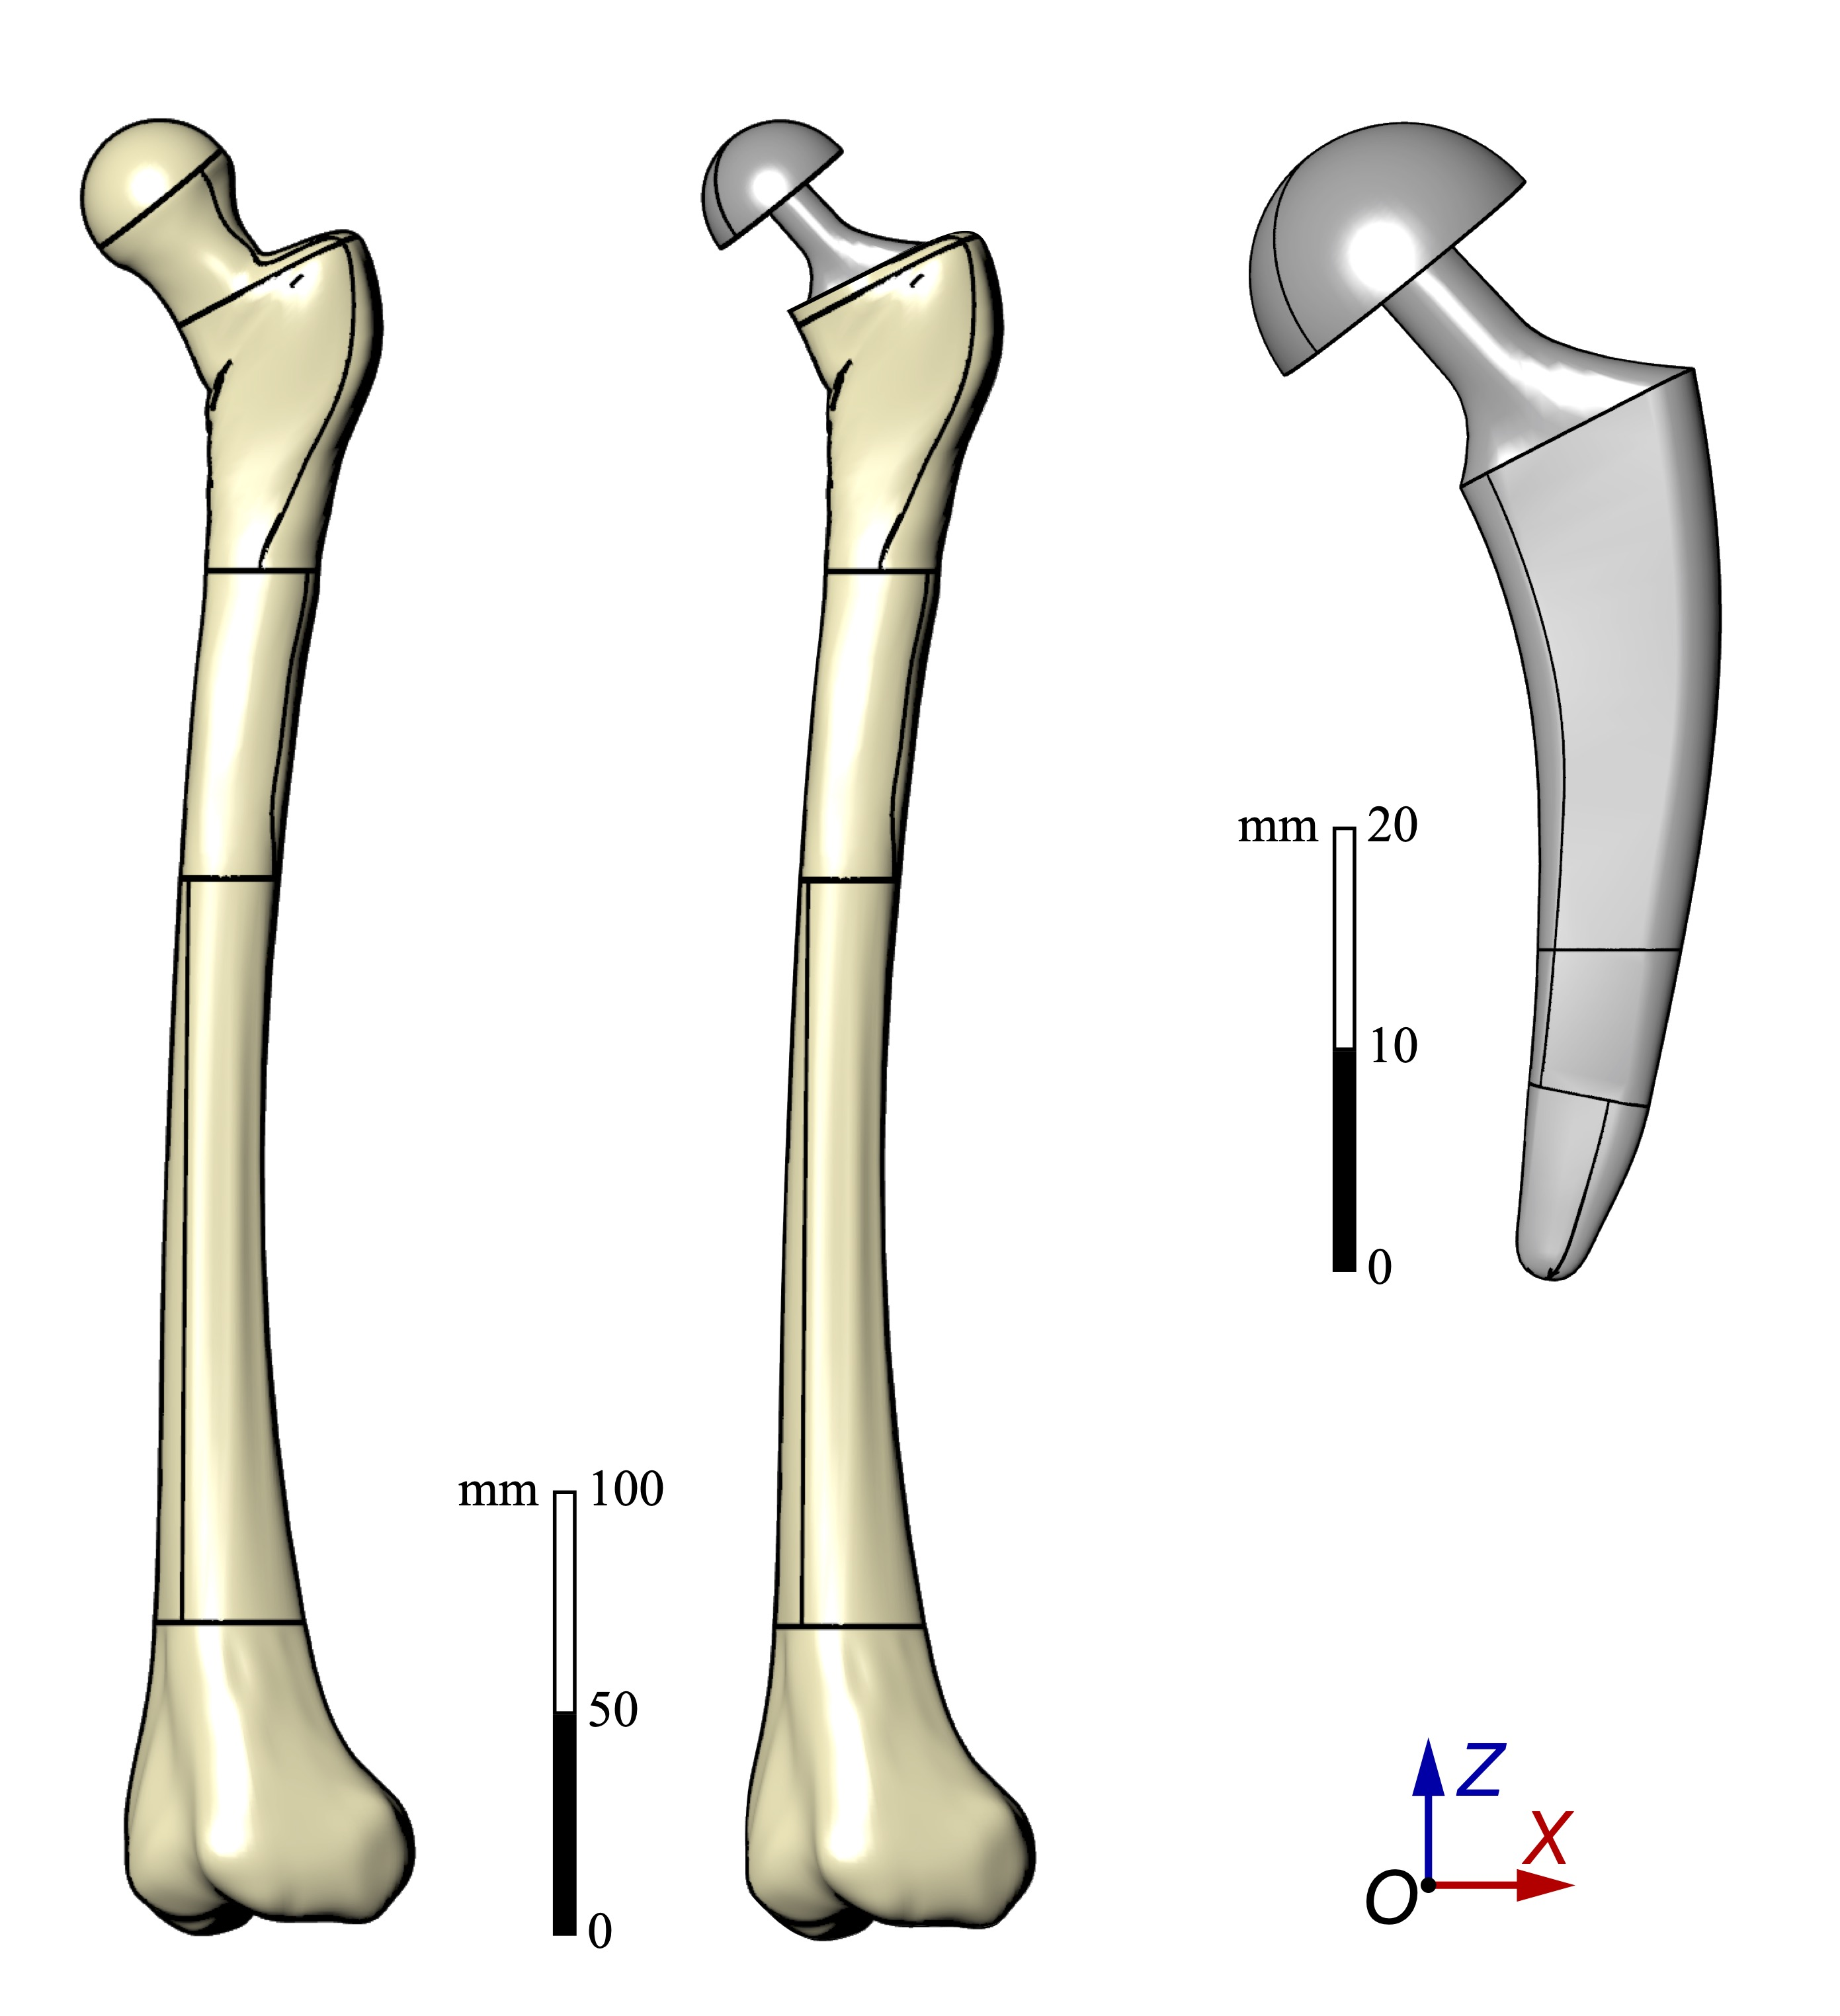
\includegraphics[width=7.3 cm]{fig/femur_geo}}
\subfigure[]{
\label{femur_fem}
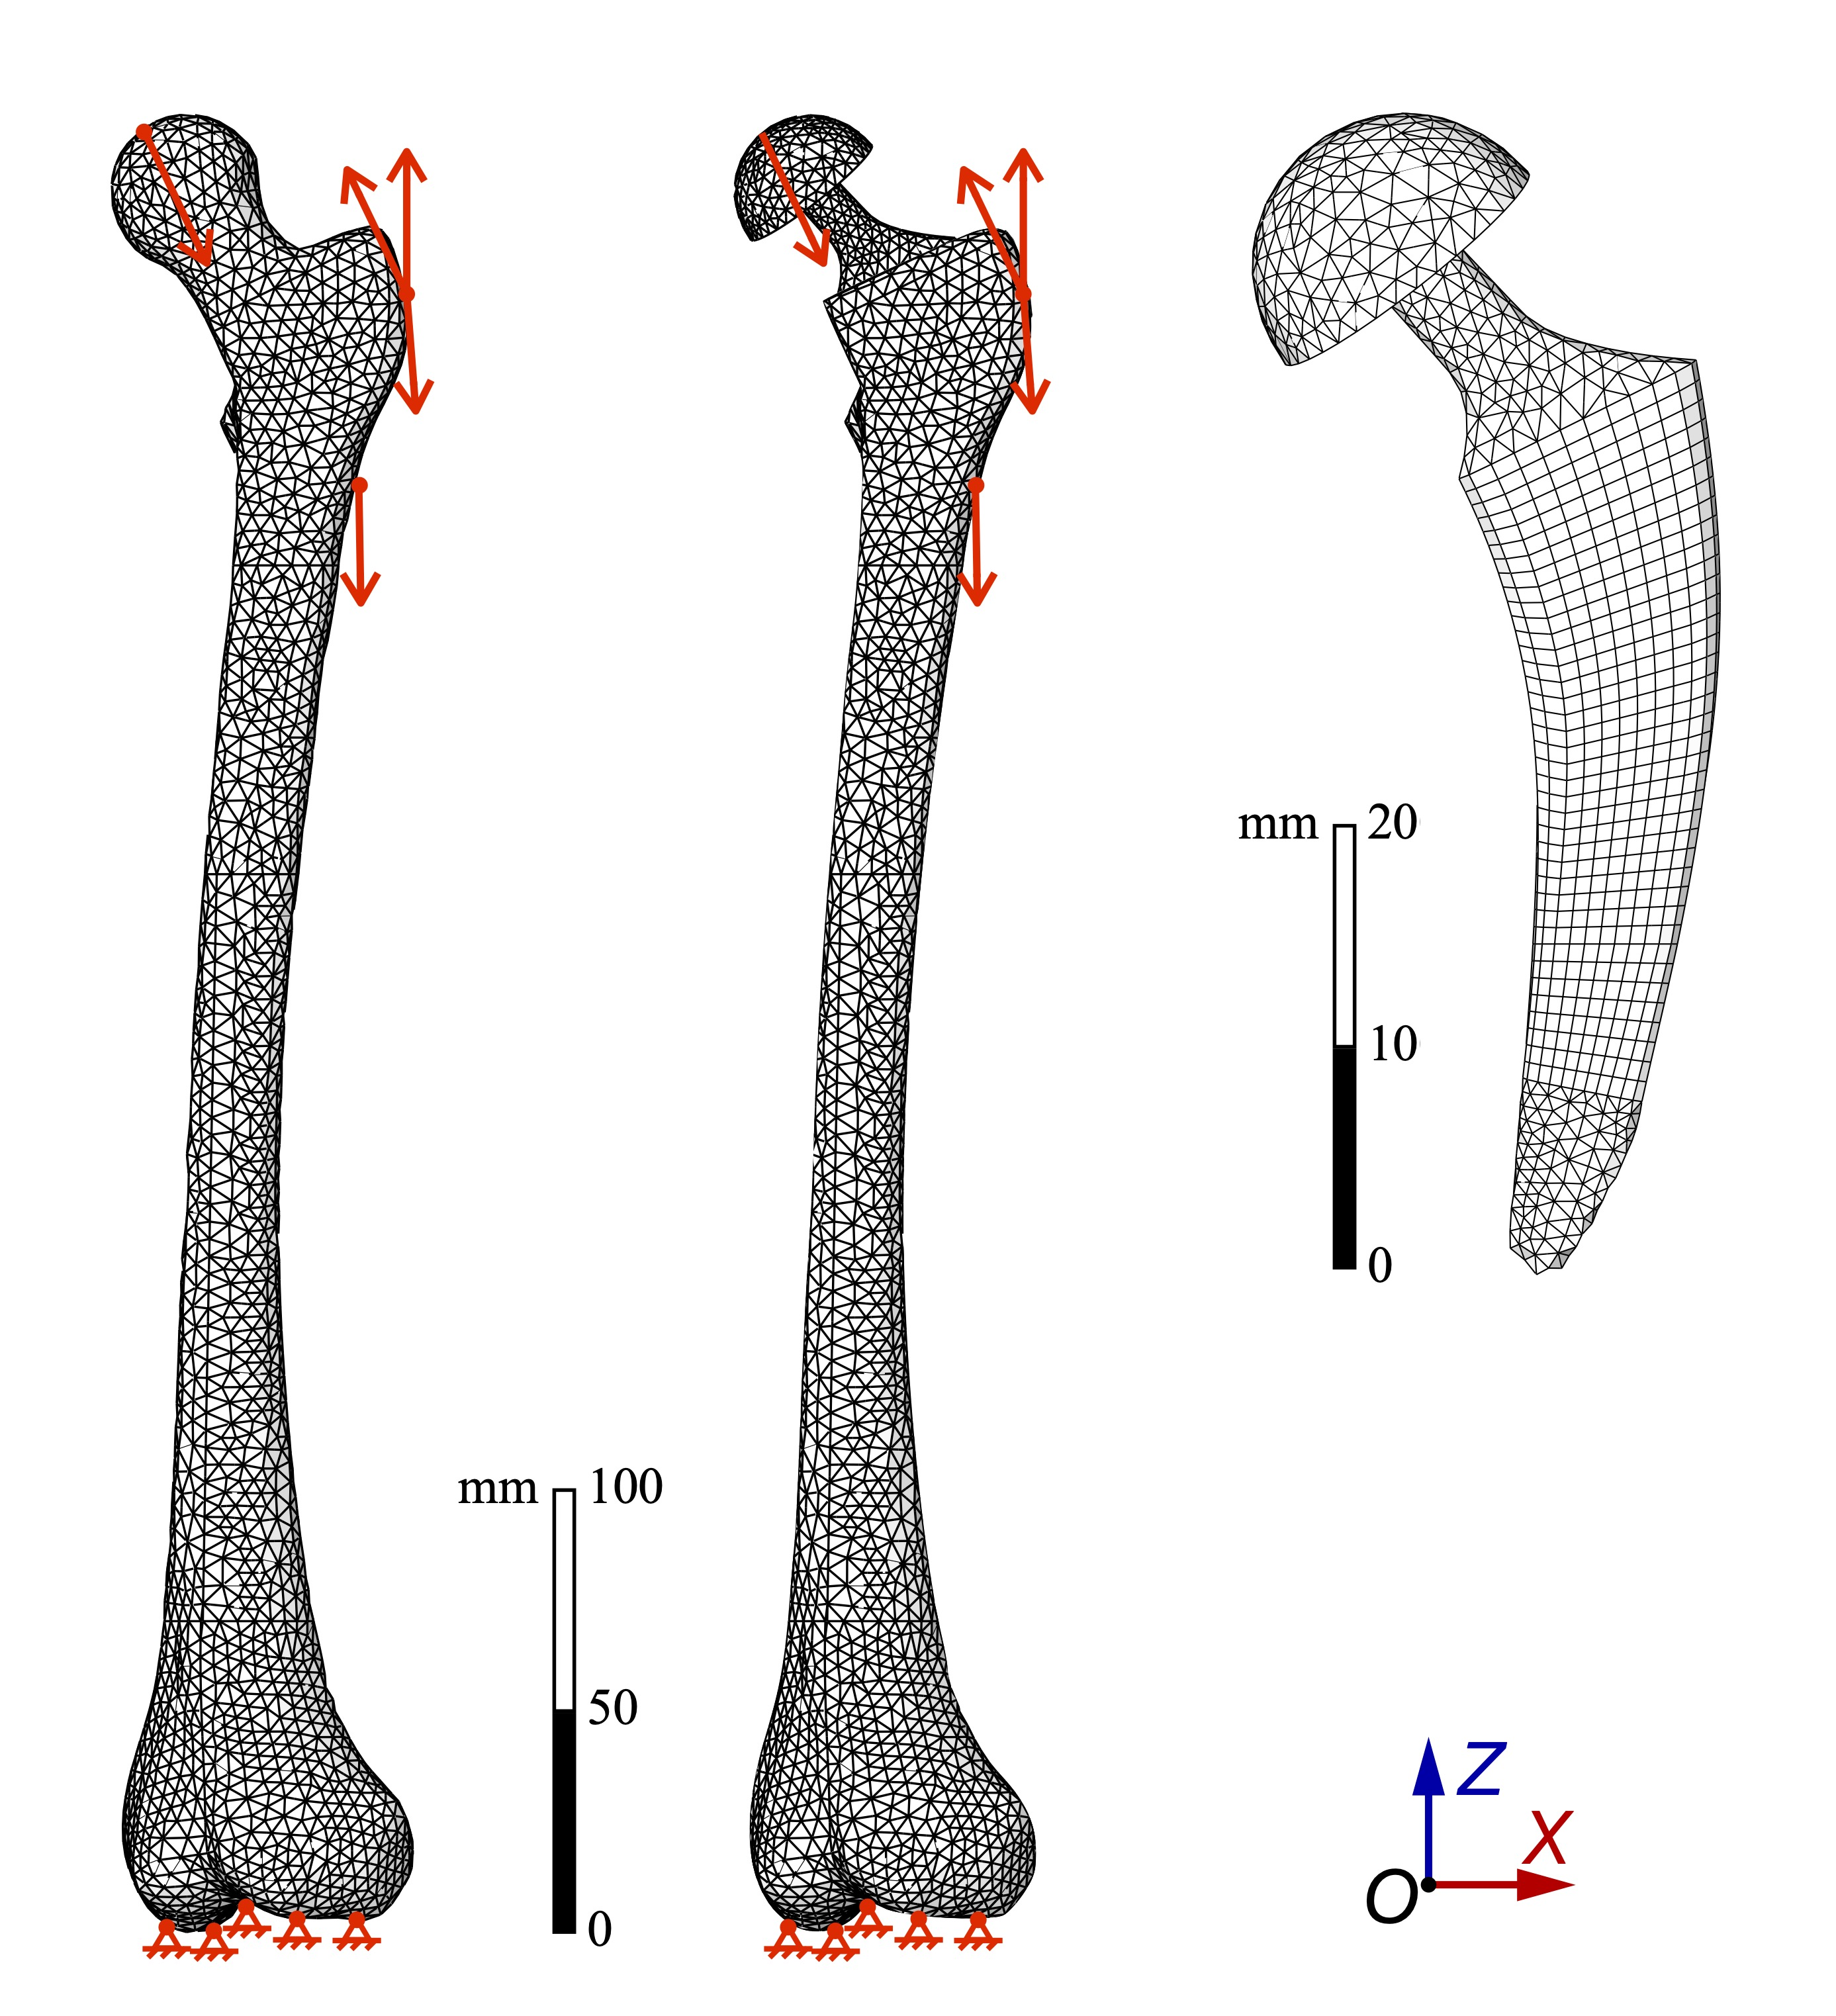
\includegraphics[width=7.3 cm]{fig/femur_fem}}
\caption{Models of pre-operative femur, implanted femur and femoral implant: (a) geometric configuration; (b) finite element model.}
\label{femur_model}
\end{figure}

The femur model is meshed with with linear tetrahedron finite elements with constraints on cell aspect ratio (0.9) and volume inhomogeneity (0.9). The size of finite element is set as 3 mm. The implant model contains two mesh zones. The implant head, neck and bottom are meshed with linear tetrahedron elements while the implant body (optimization domain) is meshed with linear hexahedron elements. The same aspect ratio and volume inhomogeneity constraints as femur mesh are applied to implant mesh. Since the minimum printing length of selective laser melting (SLM) additive manufacturing technique is 0.2 mm, the characteristic length of the hexahedron element is set as 1.5 mm so that cells with low relative density are manufacturable.\\

\subsection{Boundary conditions}

This research focuses on the general physiological loading condition in human femur. The most extreme external loadings happened on femur during the Gait circle are selected~\cite{arabnejad2017fully}. A major loading ($M_1$) is applied on the femur head (implant head) and four adductor forces ($A_1$ to $A_4$) are applied to the trochanter. Magnitudes of the loadings are shown in Table~\ref{loading}. The translational degrees of freedom on the femur bottom condyle are constraint to mimic the ankle joint structure. Since the porous implant surface stimulates osteogenic growth, it is assumed that the contacting surfaces of femur and implant are completed tied. Both rotational and translational degrees of freedom are coupled along the interface.\\

\begin{table}[htbp]
\centering
\caption{Loading condition in THA finite element model.}
\begin{tabular}{lrrr}
\hline\hline
Load & $x$-component (N) & $y$-component (N) & $z$-component (N)\\
\hline
$M_1$ & 0.0 & 0.0 & -836.0\\
$A_1$ & -58.0 & -4.3 & 86.5\\
\hline\hline
\end{tabular}
\label{loading}
\end{table}

\subsection{Trilinear interpolation}

In order to apply the predicted idealised orthotropic element properties to the distorted hexahedron element in finite element model with minimal deviation, a local coordinate generation algorithm is created based on trilinear interpolation method~\cite{kang2006three} for distorted individual finite elements in the implant optimization domain. The process is illustrated in Fig.~\ref{interpolation}. In the idealized regular hexahedron unit cell, the position of an arbitrary node $N$ inside it is denoted as:
\begin{equation}
\begin{split}
\begin{array}{ll}
p(N) = [x_N~~ y_N ~~ z_N], & x_N, y_N, z_N \in [0,1]
\end{array}
\end{split}
\label{3-1-1}
\end{equation}

The actual position of node $N$ in FE model global coordinate system is:
\begin{equation}
\begin{split}
\begin{array}{ll}
P(N) = [X_{N} ~~ Y_{N} ~~ Z_{N}], & X_{N}, Y_{N}, Z_{N} \in \mathbb{R}
\end{array}
\end{split}
\label{3-1-2}
\end{equation}

The analytical expression of $P(N)$ in terms of $p(N)$ components is:
\begin{equation}
\begin{split}
P(N) = \bm{K}^T_{\text{cube}} \cdot [1 ~~ x_N ~~ y_N ~~ z_N ~~ x_N y_N ~~ y_N z_N ~~ z_N x_N ~~ x_N y_N z_N]^T\\
\end{split}
\label{3-1-3}
\end{equation}

The parameter vector $\bm{K}_{\text{cube}}$ is defined as:
\begin{equation}
\begin{split}
\bm{K}_{\text{cube}} =
\left [ \begin{array}{rrrrrrrr}
1&0&0&0&0&0&0&0\\
-1&0&0&0&1&0&0&0\\
-1&0&1&0&0&0&0&0\\
-1&1&0&0&0&0&0&0\\
1&0&-1&0&-1&0&1&0\\
1&-1&-1&1&0&0&0&0\\
1&-1&0&0&-1&1&0&0\\
-1&1&1&-1&1&-1&-1&1
\end{array}\right ]
\left [ \begin{array}{c}
P(N_{000})\\
P(N_{001})\\
P(N_{010})\\
P(N_{011})\\
P(N_{100})\\
P(N_{101})\\
P(N_{110})\\
P(N_{111})
\end{array}\right ]
\end{split}
\label{3-1-4}
\end{equation}

Where $N_{000}$ to $N_{111}$ are the location of eight vertices in the distorted unit cell.\\

\begin{figure}[htbp]
\centering
\subfigure[]{
\label{interpolation_1}
\includegraphics[width=8 cm]{fig/interpolation_1}}
\subfigure[]{
\label{interpolation_2}
\includegraphics[width=8 cm]{fig/interpolation_2}}
\caption{Trilinear interpolation and local coordinate generation: (a) idealized regular hexahedron element; (b) distorted hexahedron element in finite element model.}
\label{interpolation}
\end{figure}

The preliminary local coordinate axes of the distorted finite element are obtained by interpolation of the original coordinates axes in idealized cubic unit cell, which are defined by vectors $\overrightarrow{N_1N_2}$, $\overrightarrow{N_3N_4}$ and $\overrightarrow{N_5N_6}$ respectively. The positions of the $N_i$ nodes in the idealized regular hexahedron unit cube are:
\begin{equation}
\begin{split}
\left\{
\begin{array}{l}
p(N_1) = [~0 ~~ 0.5 ~~ 0.5~]\\
p(N_2) = [~1 ~~ 0.5 ~~ 0.5~]\\
p(N_3) = [~0.5 ~~ 0 ~~ 0.5~]\\
p(N_4) = [~0.5 ~~ 1 ~~ 0.5~]\\
p(N_5) = [~0.5 ~~ 0.5 ~~ 0~]\\
p(N_6) = [~0.5 ~~ 0.5 ~~ 1~]\\
\end{array}
\right.
\end{split}
\label{3-1-5}
\end{equation}

The obtained preliminary principal axes are then orthogonalized to a best-fit mutually-perpendicular coordinate system for assignment of orthotropic mechanical properties. Denote the $x$ and $y$ axes of the an arbitrary orthogonal coordinates as $\overrightarrow{X^*_c}$ and $\overrightarrow{Y^*_c}$, the overall angular deviation $\varepsilon$ between orthogonal coordinates and interpolated axes is:
\begin{equation}
\begin{array}{lll}
\varepsilon & = & \varepsilon_X + \varepsilon_Y + \varepsilon_Z\\
& = & \cos^{-1}[(\overrightarrow{X^*_c}\times\overrightarrow{P_{N_1}P_{N_2}}) / (|\overrightarrow{X^*_c}|\cdot|\overrightarrow{P_{N_1}P_{N_2}}|)] + \\
& & \cos^{-1}[(\overrightarrow{Y^*_c}\times\overrightarrow{P_{N_3}P_{N_4}}) / (|\overrightarrow{Y^*_c}|\cdot|\overrightarrow{P_{N_3}P_{N_4}}|)] + \\
& & \cos^{-1}[(\overrightarrow{X^*_c}\times\overrightarrow{Y^*_c}\times\overrightarrow{P_{N_5}P_{N_6}}) / (|\overrightarrow{X^*_c}\times\overrightarrow{Y^*_c}|\cdot|\overrightarrow{P_{N_5}P_{N_6}}|)]
\end{array}
\label{3-1-6}
\end{equation}

By solving the optimization problem $\min\{\varepsilon(\overrightarrow{X^*_c}, \overrightarrow{Y^*_c})\}$, the best-fit orthogonal local coordinates $\overrightarrow{X_c}$, $\overrightarrow{Y_c}$ and $\overrightarrow{Z_c}$ are obtained, where $\overrightarrow{Z_c} = \overrightarrow{X_c} \times \overrightarrow{Y_c}$.\\

\section{Optimization framework}
\label{femur_opti}

\subsection{Objective function}
\label{femur_opti_obje}

Since the excessively high stiffness of metallic basis material is the major cause of stress shielding problem in clinical treatment, a feasible countermeasure is to reduce stiffness of the implant to make its mechanical properties approach that of femur bone tissue. In this research, the maximum global compliance of the implant is selected as the optimization target function. Compared to stiffness, compliance considers the effect of loading distribution inside implant. Location or directions with higher observed stress will be assigned with softer lattice structures. The definition of global compliance $U$ is:
\begin{equation}
U = \sum_{i=1}^N \bm{\varepsilon}_i^T\bm{C}_i\bm{\varepsilon}_i
\label{3-2-1}
\end{equation}

Where $\bm{\varepsilon}$ is element strain tensor, $\bm{C}$ is element constitutive matrix and $N$ is the amount of elements in optimization domain.\\

\subsection{Constraint conditions}
\label{femur_opti_cons}

Constraint conditions considered in the topology optimization design include structural failure criteria, bone growth stimulation, additive manufacturing (AM) capability and implant material fraction.\\

\subsubsection{Structural failure criteria}

To avoid structural failure in lattice cells with low relative density, the Tsai-Wu failure criteria is checked during each iteration. For material with identical compressive and tensile strength, the definition of Tsai-Wu safety factor SF is calculated as~\cite{tsai1971general}:
\begin{equation}
\text{SF} = 1 / (\sum_{i=1}^{3}F_{ii}s_{ii}^2 + F_{44}s_{23}^2 + F_{55}s_{13}^2 + F_{66}s_{12}^2)  \geq 1
\label{3-2-2}
\end{equation}

Where $\bm{F}$ are Tsai-Wu parameters calculated from compressive, shear, equibiaxial strength and $\bm{s}$ is the stress tensor of individual element:
\begin{equation}
\left\{
\begin{array}{llll}
F_{ii} & = \frac{1}{{\sigma}^2_{ii}} & \text{for} & i \in [~1,~2,~3~]\\
F_{44} & = \frac{1}{{\tau}_{23}^2} & &  \\
F_{55} & = \frac{1}{{\tau}_{13}^2} & & \\
F_{66} & = \frac{1}{{\tau}_{12}^2} & & \\
\end{array}
\right.
\label{2-1-20}
\end{equation}
\begin{equation}
\bm{s} = [~s_{11} ~~ s_{22} ~~ s_{33} ~~ s_{23} ~~ s_{13} ~~ s_{12}~]^T
\label{3-2-3}
\end{equation}

\subsubsection{Bone growth stimulation and AM capability}

To stimulate new bone formation and osteo-integration surrounding implant, the pore size of the unit cells on bone-implant contact surface is restricted to be $50 - 800$~{\textmu}m\cite{harrysson2008direct}. The minimum strut radius of all lattice cells is set to be 200~{\textmu}m in consideration of the SLM additive manufacturing capability~\cite{de2013bone}. The constraint of growth and manufacturing requirements are determined prior to optimization process and are reflected by the strut range assigned to individual unit cells. Since cells with different anisotropy pattern have different strut radius with same relative density, as a conservative design method, the radius ratio $x_1:x_2:x_3  = 1:3:3$ is applied in default to analyze the radius-porosity relationship.\\


\subsubsection{Material removal fraction}
\label{to_con_mrf}
The implant material fraction $\tilde{\rho}$ is defined as the ratio of material volume in optimization domain to the bulk volume of optimization domain:
\begin{equation}
\tilde{\rho} = \frac{\sum_{i=1}^N{\rho_iV_i}}{\sum_{i=1}^N{V_i}}\\
\label{3-3-1}
\end{equation}

A target implant material fraction $\hat{\rho}$ is pre-determined as a design requirement. During optimization design, the material fraction is allowed to deviate from the target value within 2\%:
\begin{equation}
0.98\hat{\rho} \leq \tilde{\rho} \leq 1.02\hat{\rho}\\
\label{3-3-2}
\end{equation}


\subsection{Optimization algorithm}

MMA algorithm~\cite{svanberg1987method} is selected to solve the maximum compliance optimization problem described in Section~\ref{femur_opti_obje} and~\ref{femur_opti_cons} for its stable and rapid convergence process. The algorithm converts target function and constraint conditions into approximating convex function and finds the optimal solution via gradient searching. The general form of optimization problem acceptable by MMA is:
\begin{equation}
\begin{array}{llll}
\text{maximise} & f_0(\{x\})\\
\text{subject to} & \bm{f}(\{x\}) \leq \hat{\bm{f}}\\
& x_i^- \leq x_{i} \leq x_i^+ & \text{for} & x_i \in \{x\}\\
\end{array}
\label{3-4-1}
\end{equation}

Where $f_0$ is the target function, $\bm{f}$ and $\hat{\bm{f}}$ are list of constraint functions and constraint constants. Their gradients against design variable, $\partial f_0 / \partial \{x\}$ and $\partial \bm{f} / \partial \{x\}$ are required for optimization computation.\\

In this research, the mathematical expression of the maximum compliance topology optimization problem is:
\begin{equation}
\begin{array}{llll}
\text{maximise} & U(\{\bm{x}\})\\
\text{subject to} & 1/(\text{SF}_i) \leq 1 & \text{for} & i = 1, 2,\cdots N\\
& -\tilde{\rho} \leq -0.98\hat{\rho}\\
& \tilde{\rho} \leq 1.02\hat{\rho}\\
& \rho_i^- \leq \rho_{i} \leq \rho_i^+ & \text{for} & i = 1, 2,\cdots N\\
\end{array}
\label{3-4-2}
\end{equation}

Where $\{\bm{x}\}\in\mathbb{R}_+^{N\times3}$ is the orthotropic strut radii assigned to unit cells in optimization domain, $\{\rho^-\}\in\mathbb{R}_+^N$ and $\{\rho^+\}\in\mathbb{R}_+^N$ are lower and upper bounds of unit cell relative density in optimization domain.\\

The termination criteria of optimization iteration process is triggered upon the convergency of global compliance. To avoid fake convergence, both 5-step compliance change and 1-step compliance change are considered. At $i$ th step ($i \geq 10$), the criteria is calculated as:
\begin{equation}
\text{t.c.} = \max{\{ \frac{U_i-U_{i-1}}{U_{i-1}},~~ \frac{\sum_{i-4}^{i} U_j-\sum_{i-9}^{i-5}U_j}{\sum_{i-9}^{i-5}U_j} \}}
\label{3-4-7}
\end{equation}

\subsection{Sensitivity analysis}

During MMA iteration process, gradient of global compliance against all design variables are required. In order to calculate the gradient promptly, its analytic expression is constructed. Generally, in the scope of implant entity, the global compliance is defined as:
\begin{equation}
U = \bm{D}^T\bm{K}\bm{D}
\label{3-4-T1}
\end{equation}

Where $\bm{D}$ is the global boundary displacement vector and $\bm{K}$ is the global stiffness matrix. Take the partial derivative on the two side of Equation~\ref{3-4-T1} against one random design vector $x_i$:
\begin{equation}
\frac{\partial U}{\partial x_i} = 2\bm{D}^T\bm{K}\frac{\partial \bm{D}}{\partial x_i} + \bm{D}^T\frac{\partial \bm{K}}{\partial x_i}\bm{D}
\label{3-4-T2}
\end{equation}

Ignoring the body force of implant, the global boundary force vector $\bm{Q}$ is defined as:
\begin{equation}
\bm{Q} = \bm{K}\bm{D} 
\label{3-4-T3}
\end{equation}

Take the partial derivative on the two side of Equation~\ref{3-4-T3} against $x_i$:
\begin{equation}
\frac{\partial \bm{Q}}{\partial x_i} = \frac{\partial \bm{K}}{\partial x_i}\bm{D} + \bm{K}\frac{\partial \bm{D}}{\partial x_i}
\label{3-4-T4}
\end{equation}

Considering the global boundary force vector is not influenced by adjustment of design variables ($\partial \bm{Q} / \partial x_i = 0$), Equation~\ref{3-4-T4} is further simplified as:
\begin{equation}
\frac{\partial \bm{D}}{\partial x_i} = -\bm{K}^{-1}\frac{\partial \bm{K}}{\partial x_i}\bm{D}
\label{3-4-T5}
\end{equation}

Substitute Equation~\ref{3-4-T5} into Equation~\ref{3-4-T2}:
\begin{equation}
\frac{\partial U}{\partial x_i} = -\bm{D}^T\frac{\partial \bm{K}}{\partial x_i}\bm{D}
\label{3-4-T6}
\end{equation}

In microstructure scope, Equation~\ref{3-4-T6} is expressed as:
\begin{equation}
\frac{\partial U}{\partial x_i} = -\sum\bm{d}_i^T\frac{\partial \bm{k}_i}{\partial x_i}\bm{d}_i = -\bm{\varepsilon}_i^T\frac{\partial \bm{C}_i}{\partial x_i}\bm{\varepsilon}_i
\label{3-4-T7}
\end{equation}

Where $\bm{d}_i$, $\bm{k}_i$, $\bm{\varepsilon}_i$ and $\bm{C}_i$ are the local boundary displacement vector, local constitutive matrix, local strain vector and local stiffness matrix of i-th element.\\

Equation~\ref{3-4-T7} reveals that the variation of global compliance is solely caused by stiffness matrix change in each element. The gradient is hence calculated by linear approximation:
\begin{equation}
\frac{\partial U}{\partial x_i} \doteq -\frac{\bm{\varepsilon}_i^T[\bm{C}_i(x_i + \Delta x_i^+) - \bm{C}_i(x_i - \Delta x_i^-)]\bm{\varepsilon}_i}{\Delta x_i^+ + \Delta x_i^-}
\label{3-4-3}
\end{equation}

The element Tsai-Wu safety factor $\text{SF}_i$ is only dependent on the architecture of local element $i$. Hence $\partial (1/\text{SF}_i) / \partial x_j = 0$ for $i \neq j$. The gradient of element safety factor again the local design variable $x_i$ is the calculated as:
\begin{equation}
\frac{\partial (1/\text{SF}_i)}{\partial x_i} \doteq \frac{\text{SF}_i(x_i - \Delta x_i^-) - \text{SF}_i(x_i + \Delta x_i^+)}{(\Delta x_i^+ + \Delta x_i^-)\text{SF}_i(x_i + \Delta x_i^+) \text{SF}_i(x_i - \Delta x_i^-)}
\label{3-3-7}
\end{equation}

The constitutive matrix $\bm{C}_i$ and safety factors $\text{SF}_i$ of individual element are calculated from prediction function $\bm{Y}^*(\bm{x}^*)$ in Equation~\ref{2-1-15}, Equation~\ref{2-1-18} and Equation~\ref{3-2-2}.\\

According to Equation~\ref{3-3-1}, the gradient of implant material fraction against unit cell strut radius is:
\begin{equation}
\frac{\partial \tilde{\rho}}{\partial x_i} \doteq \frac{V_i[\rho_i(x_i + \Delta x_i^+)-\rho_i(x_i - \Delta x_i^-)]}{(\Delta x_i^+ + \Delta x_i^-)\sum_{j=1}^N V_j}
\label{3-4-6}
\end{equation}

During the iteration trials, the finite decrement and increment of design variables for linear approximation are defined as:
\begin{equation}
\left\{
\begin{array}{l}
\Delta x_i^- = \min\{0.005,~x_i\}\\
\Delta x_i^+ = \min\{0.005,~1 - x_i\}\\
\end{array}
\right.
\label{3-4-7}
\end{equation}

\section{Performance evaluation}
\label{femur_perf}

The bio-mechanical performance of optimized femoral implant is quantitatively evaluated by comparison of femur stress condition before and after implantation. Two indicators, resorbed bone mass fraction (mbr)~\cite{kuiper1992numerical} and stress shielding intensity (ssi)~\cite{boyle2011comparison}, are selected as indicators of post-operative bone degeneration.\\

The calculation of resorbed bone mass fraction assumes that bone tissue degeneration happens when stress reduction is higher 30\%. The mass fraction of bone tissue suffering high risk of degeneration among the entire femur domain is calculated as:
\begin{equation}
\text{mbr} = \frac{\sum_{i=1}^N \rho_{m,i}V_i [1- \theta(\max\{\frac{s_{v, \text{ref}, i} - s_{v,i}}{s_{v,\text{ref},i}}~,~0\}-30\%)]}{\sum_{i=1}^n \rho_{m,i}V_i}
\label{5-2-1}
\end{equation}

Where $\theta$ represents approximated Heaviside step function:
\begin{equation}
\theta(x) = 1 / (1 + e^{-200x})
\label{5-2-T1}
\end{equation}

Stress shielding severityindicator reflects the average severity of bone tissue degeneration in vertebrae domain. Its definition is:
\begin{equation}
\text{ssi} = \frac{\sum_{i=1}^N \rho_{m,i}V_i \max\{(s_{v, \text{ref}, i} - s_{v,i}) / (s_{v,\text{ref},i})~,~0\}}{\sum_{i=1}^n \rho_{m,i}V_i}
\label{4-5-T1}
\end{equation}


\subsection{Iteration history}

At iteration step 0, the relative density and anisotropy pattern of all unit cells in optimization domain are set to be 50\% and isotropic ($x_1:x_2:x_4 = 1:1:1$). The compliance variation of graded-density isotropic and anisotropic lattice implants during iteration process are shown in Fig.~\ref{history_compliance}. Their compliances converge at 29.243 mJ and 40.622 mJ respectively, achieving 112.5\% and 195.2\% increment compared to 13.763 mJ in uniform-density isotropic implant. The introduction of anisotropic lattice microstructures enhances stiffness-reduction performance.\\

The resorbed bone mass fraction in femur with uniform-density isotropic implant and fulfilled solid implant are 3.483\% and 17.413\% respectively. Fig.~\ref{history_mbr} shows its variation during iteration. Compared with uniform-density implant, graded-density implant with isotropic and anisotropic microstructure reduce the resorption fraction by 13.4\% ($\text{mbr} = 3.015\%$) and 47.5\% ($\text{mbr} = 1.827\%$) respectively. The evaluation results reveal that a more satisfactory stress shielding moderation effect is achieved by anisotropic lattice implant.\\

Similar variation process is observed on stress shielding intensity in femur. At convergence, the isotropic and anisotropic graded-density femoral implant lead to 2.847\% and 1.661\% overall stress reduction in the femur, which is 35.1\% and 62.1\% lower than ssi in 50\% uniform-density implant (4.387\%). Compared with solid implant (8.700\%), the ssi is reduced by 62.3\% and 80.9\% respectively.\\



\begin{figure}[htbp]
\centering
\subfigure[]{
\label{history_compliance}
\includegraphics[width=7.3 cm]{fig/history_compliance}}
\subfigure[]{
\label{history_mbr}
\includegraphics[width=7.3 cm]{fig/history_mbr}}
\subfigure[]{
\label{history_ssi}
\includegraphics[width=7.3 cm]{fig/history_ssi}}
\caption{Evolutional history of optimization objective function and bio-mechanical performance indicator: (a) global compliance of implant; (b) resorbed bone mass fraction of femur; (c) stress shielding severity of femur.}
\label{history}\end{figure}


\subsection{Optimal lattice implant design}

Fig.~\ref{density} shows differentiated relative density distribution in optimized isotropic and anisotropic lattice implant. For graded-density implant with isotropic microstructures, the distribution of unit cell porosity corresponds well to the stress condition in pre-optimization implant (Fig.~\ref{stress_solid}). Generally, the algorithm moves material from unit cells with higher stress (e.g. the front and back edge of the implant) to unit cells with lower stress (e.g. the central column of implant), so that to guarantee the compliance increment caused by unit cell material removal is always higher than compliance reduction caused by commensurate material increment in counterpart cells. The net global compliance hence increases in each iteration step. For graded-density implant with anisotropic unit cells, a high relative density zone appears at the upper middle of the implant, close to the back of the implant. However, the relative density differentiation in anisotropic implant is not as significant as in isotropic implant. This is caused by material re-allocation among different coordinate directions. Albeit the radii of struts along high stress direction are reduced, materials are assigned to the struts along other directions in those unit cells. Therefore, the variation of unit cell relative density in anisotropic implant is not apparent compared to isotropic implant.\\

\begin{figure}[htbp]
\centering
\subfigure[]{
\label{density_isot}
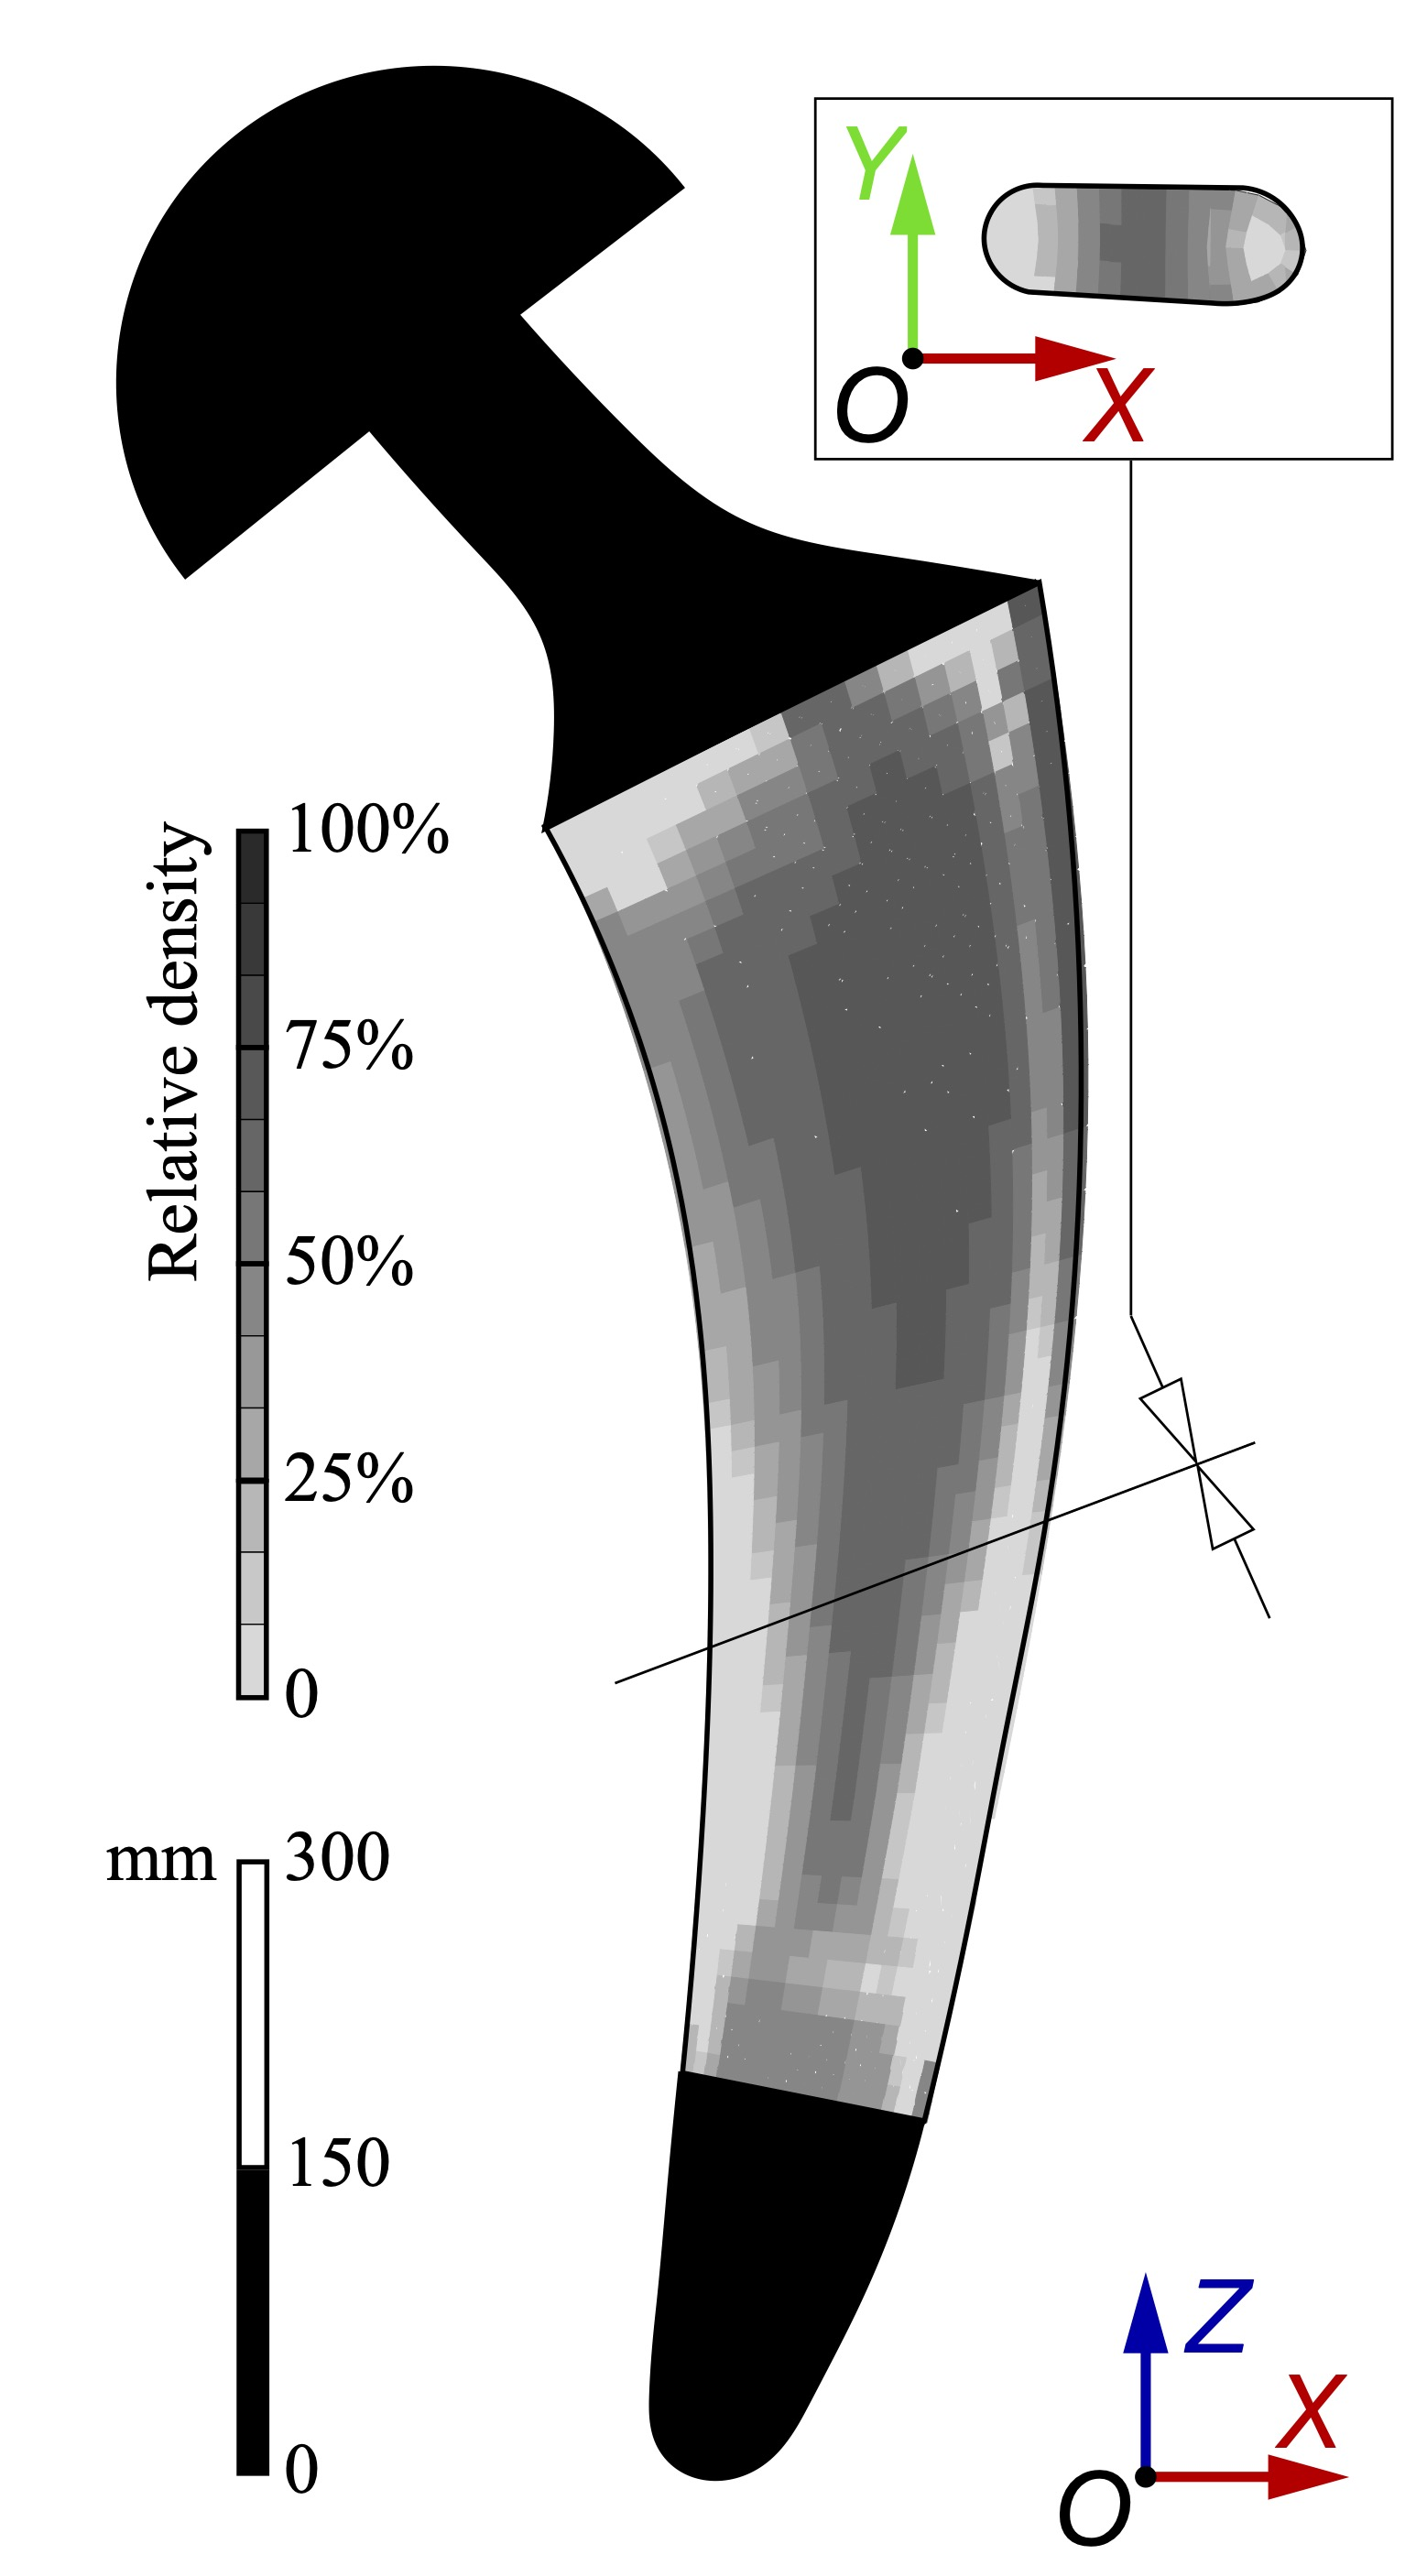
\includegraphics[width=7.3 cm]{fig/density_isot}}
\subfigure[]{
\label{density_anis}
\includegraphics[width=7.3 cm]{fig/density_anis}}
\caption{Optimal design of lattice implant: (a) distribution of unit cell relative density in implant with isotropic microstructures; (b) distribution of unit cell relative density in implant with anisotropic microstructures.}
\label{density}
\end{figure}

To clearly visualize the microstructure anisotropy arrangement, Fig.~\ref{anis} plots the cross-sectional contours of unit cell lattice struts along $x$, $y$ and $z$ direction in optimized graded-density femoral implant with anisotropic microstructures. For strut along $x$ and $y$ directions, the variation mainly happens at three areas: the top, the front edge and the back bottom of the implant. In these three areas, both thick and thin strut radii are observed. While for unit cells at the central column of the implant, the variation of their radii along $x$ and $y$ directions are not obvious. Most radii are close to 0.302 mm, with which the 50\% relative density. However, for struts along $z$ direction, the graded distribution of strut thickness is apparent. A column with high radius thickness appears at the center of the implant. While for unit cells at the front and back edge, extremely think vertical struts with radius value lower than 0.1 unit cell side length is observed.\\


\begin{figure}[htbp]
\centering
\subfigure[]{
\label{anis_x}
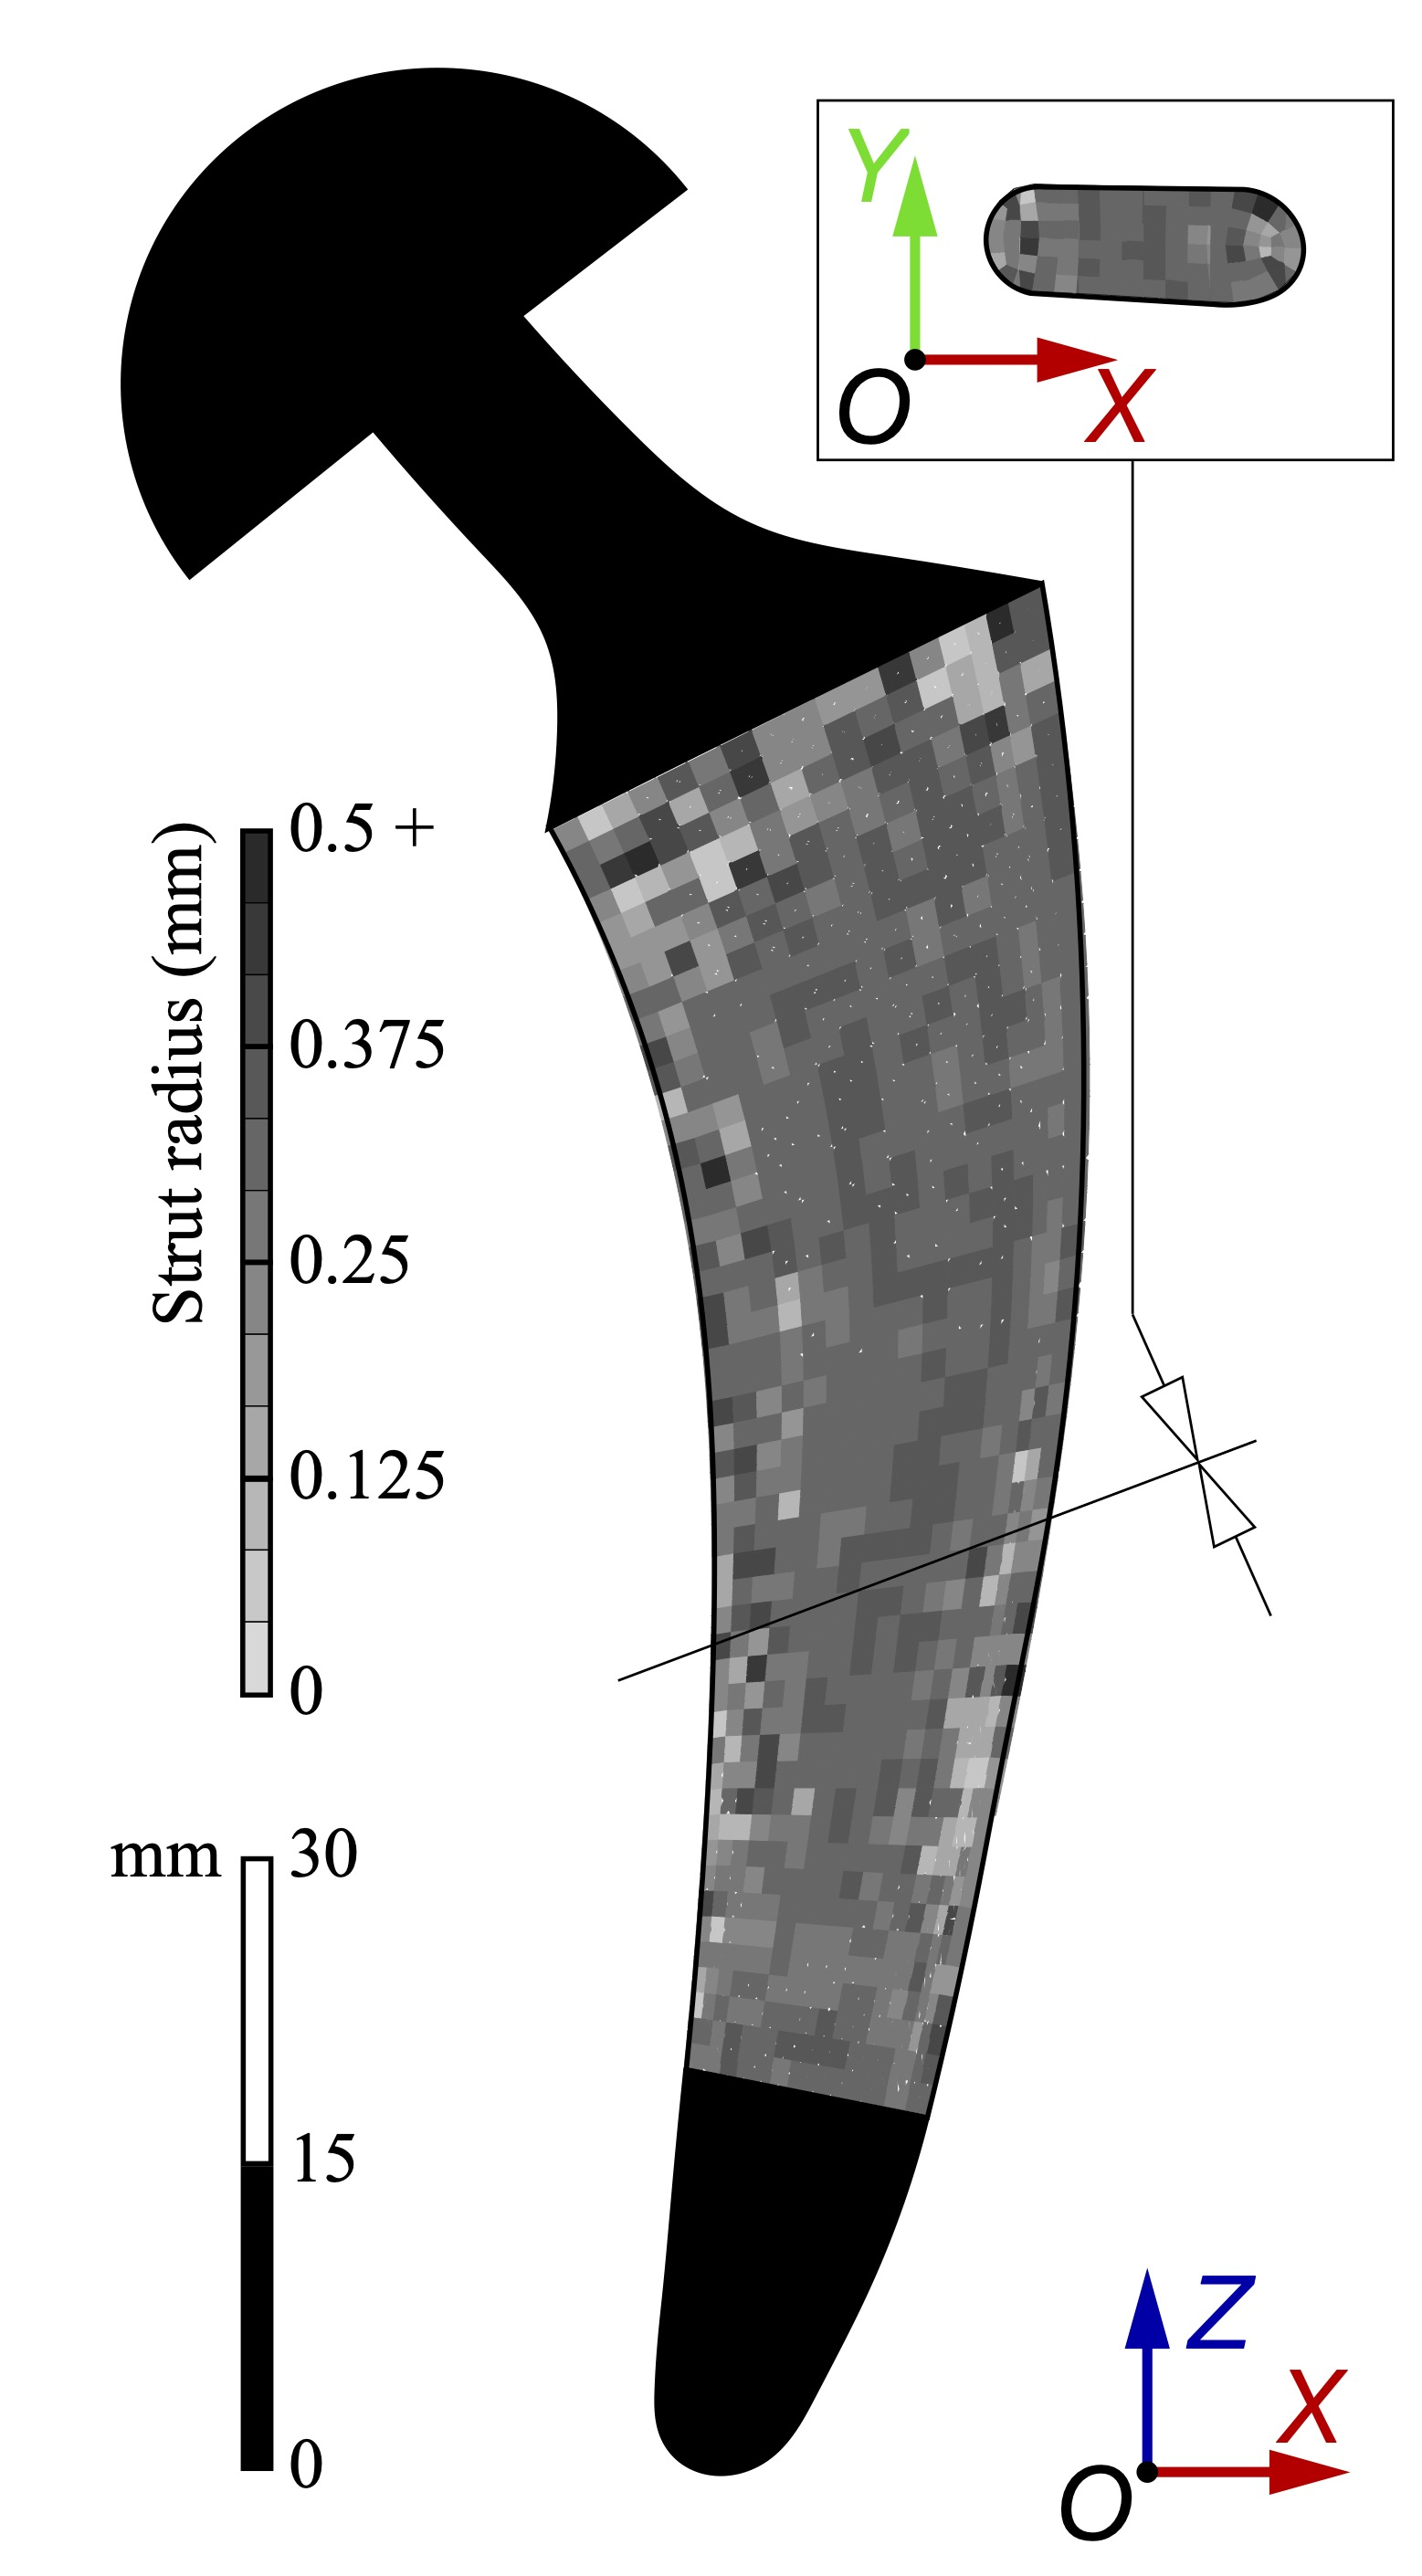
\includegraphics[width=4.7 cm]{fig/anis_x}}
\subfigure[]{
\label{anis_y}
\includegraphics[width=4.7 cm]{fig/anis_y}}
\subfigure[]{
\label{anis_z}
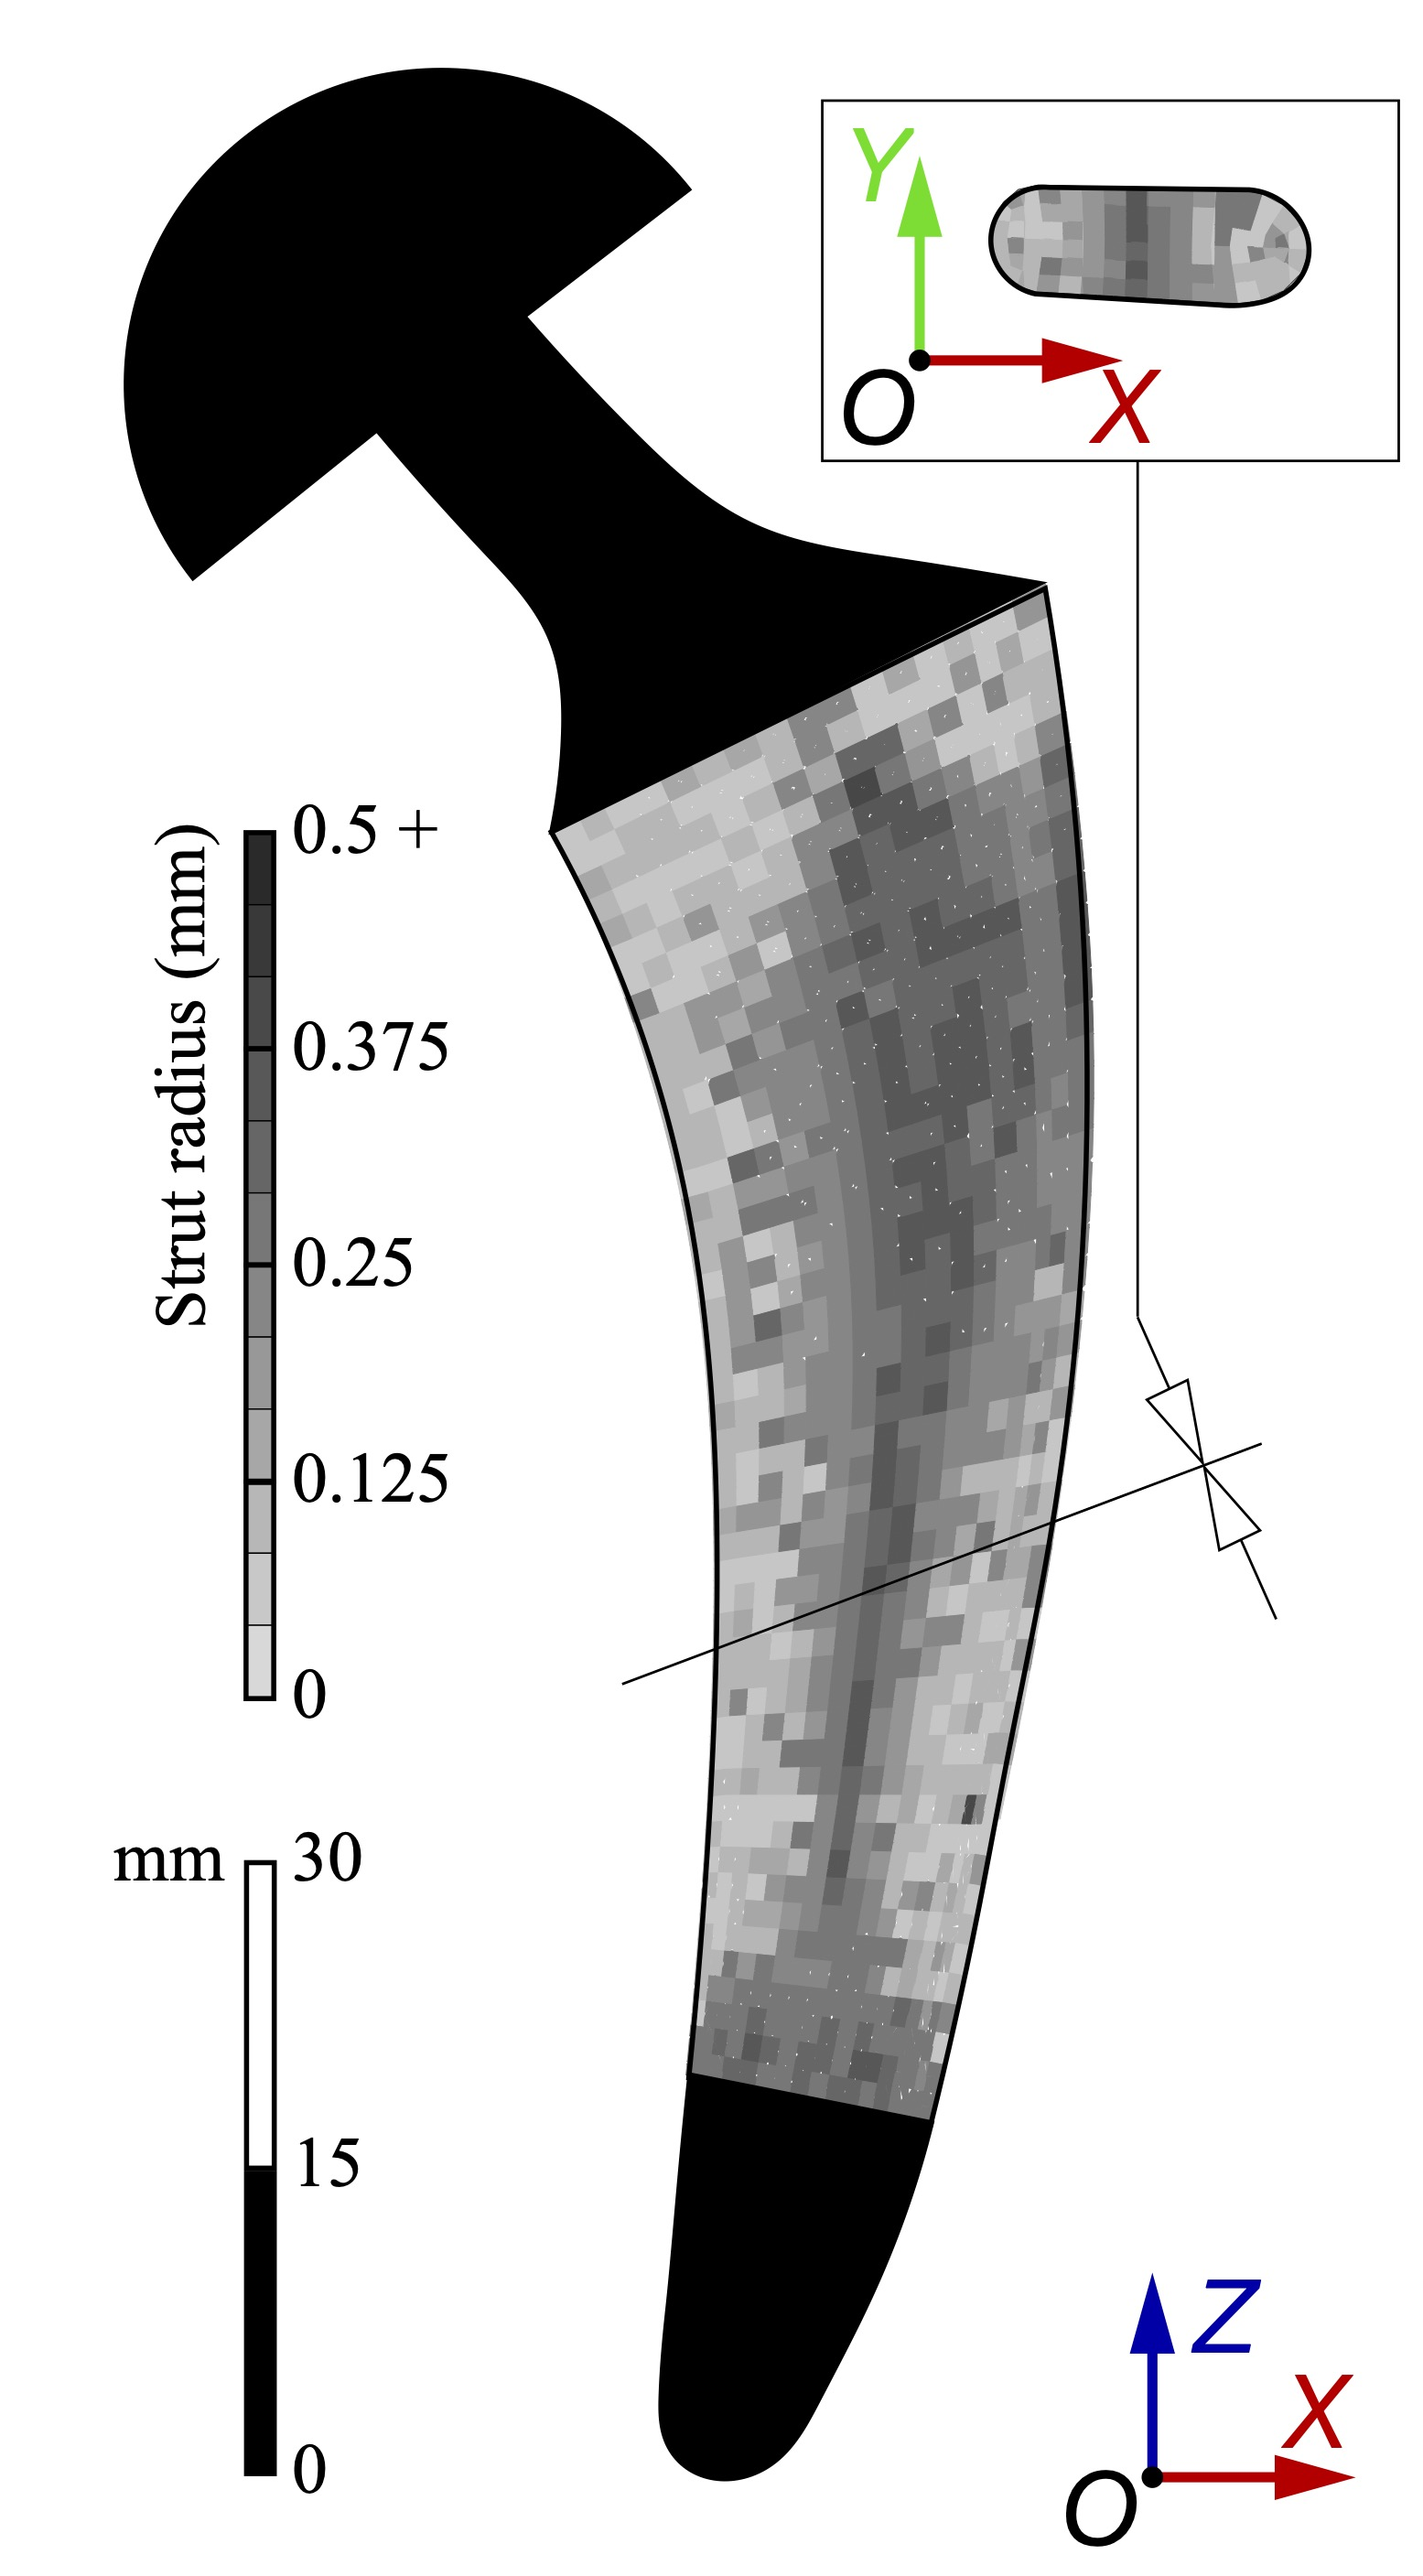
\includegraphics[width=4.7 cm]{fig/anis_z}}
\caption{Distribution of unit cell strut radii in implant with anisotropic microstructures: (a) along $x$ direction; (b) along $y$ direction; (c) along $z$ direction.}
\label{anis}
\end{figure}

Comparison between Fig.~\ref{anis} and Fig.~\ref{component} manifests that the anisotropic unit cell architectures match well with the anisotropic stress condition in pre-optimization implant. Generally, basis materials are allotted from high stress directions to low stress directions, so that the overall resistance to the anisotropic stress condition in the unit cells is minimized and a higher global compliance is achieved. As an example, for unit cells nearby the front and back edge of the implant, the strongest stress happens along vertical direction since the body load is applied vertically (Fig.~\ref{s33})). Correspondingly, the lattice unit cells at these positions are assigned with weakened $z$ directional struts (Fig.~\ref{anis_z}) to ease the local deformation and increment of cell compliance. Similarly, high $s_{13}$ values appeared on the back bottom of optimization domain causes weakened $y$-directional cell struts.\\

\begin{figure}[htbp]
\centering
\subfigure[]{
\label{s11}
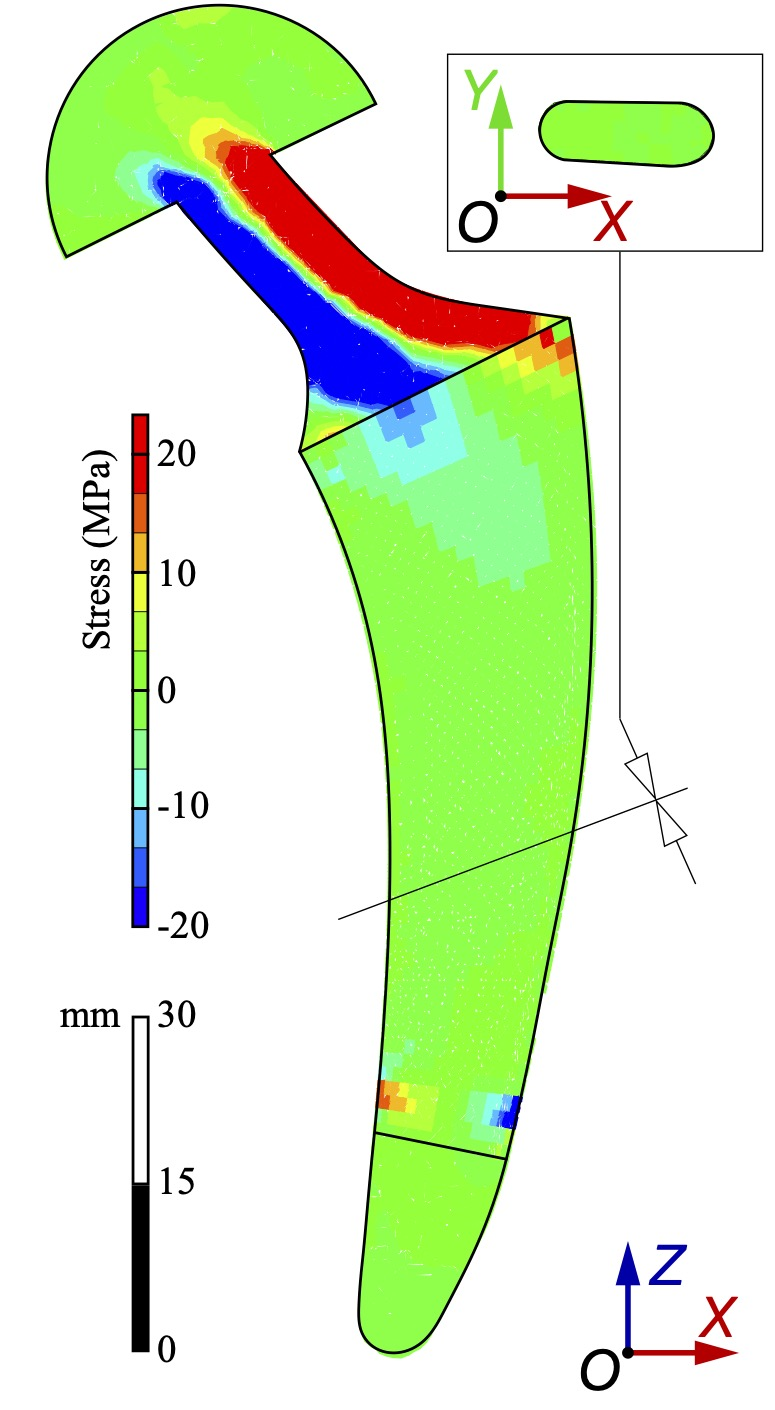
\includegraphics[width=4 cm]{fig/s11}}
\subfigure[]{
\label{s22}
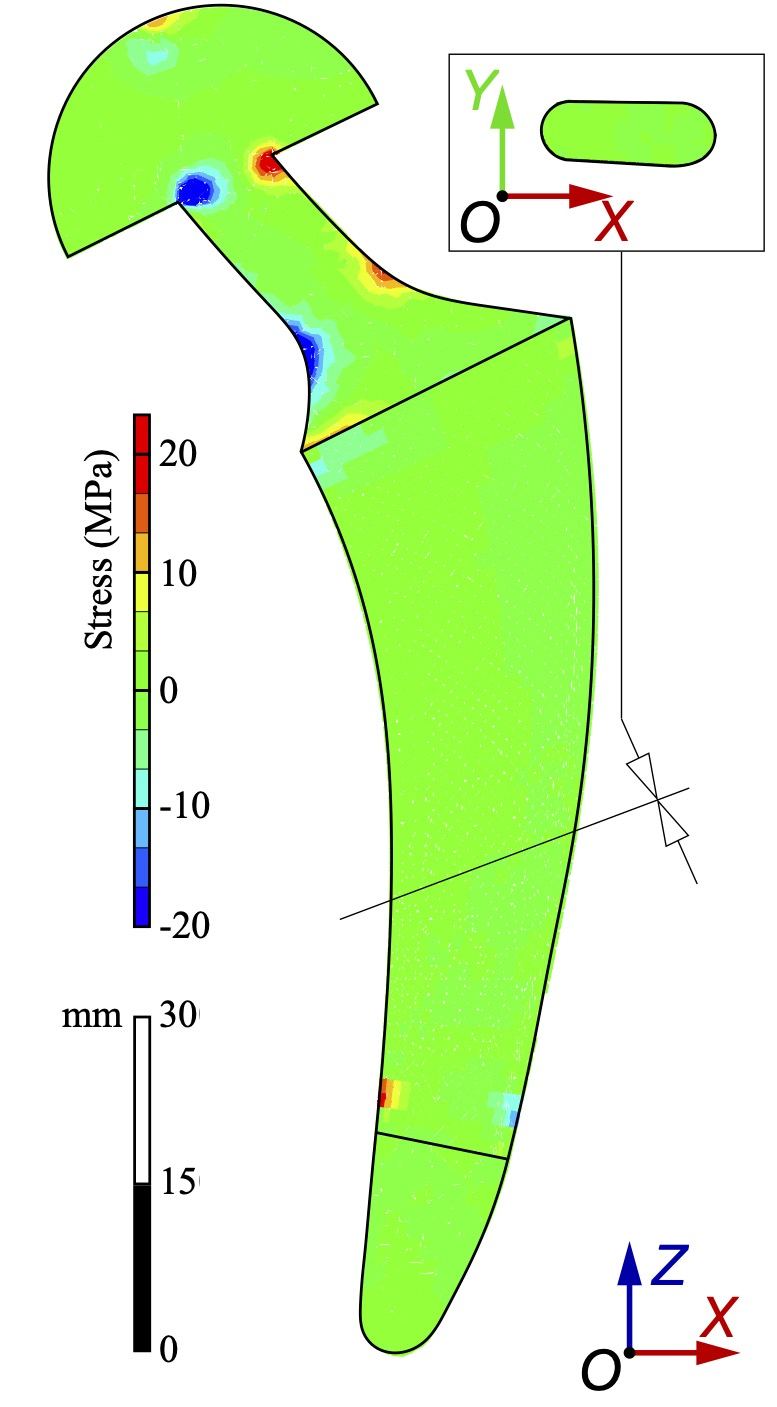
\includegraphics[width=4 cm]{fig/s22}}
\subfigure[]{
\label{s33}
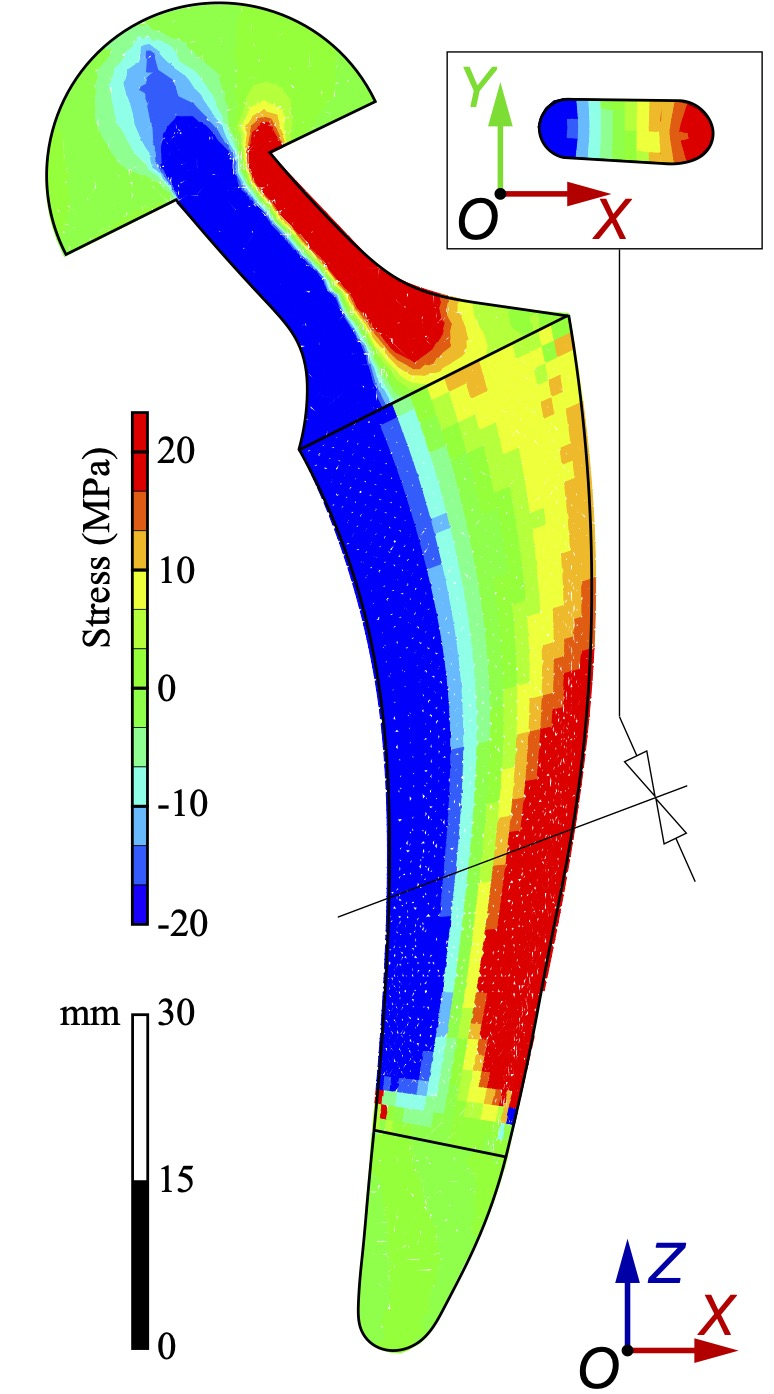
\includegraphics[width=4 cm]{fig/s33}}
\subfigure[]{
\label{s23}
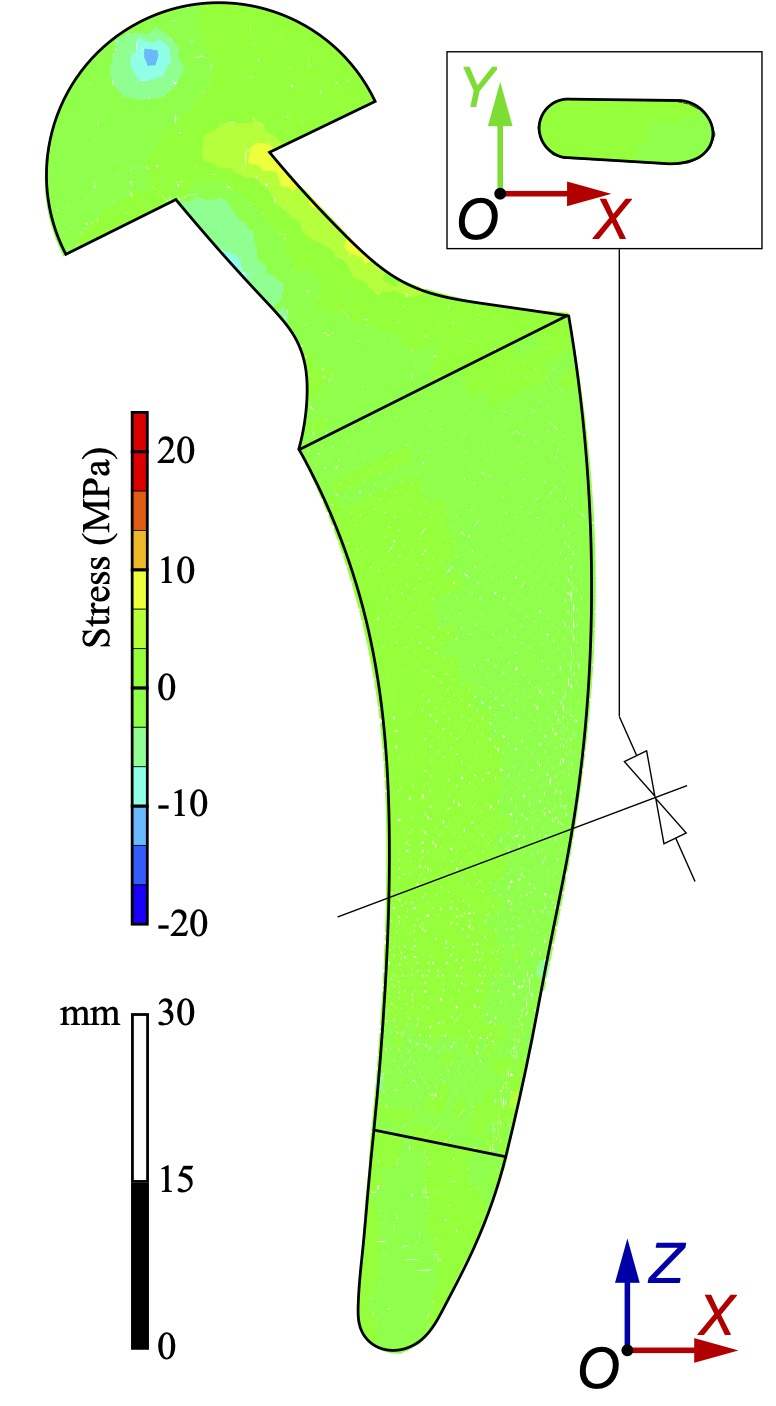
\includegraphics[width=4 cm]{fig/s23}}
\subfigure[]{
\label{s13}
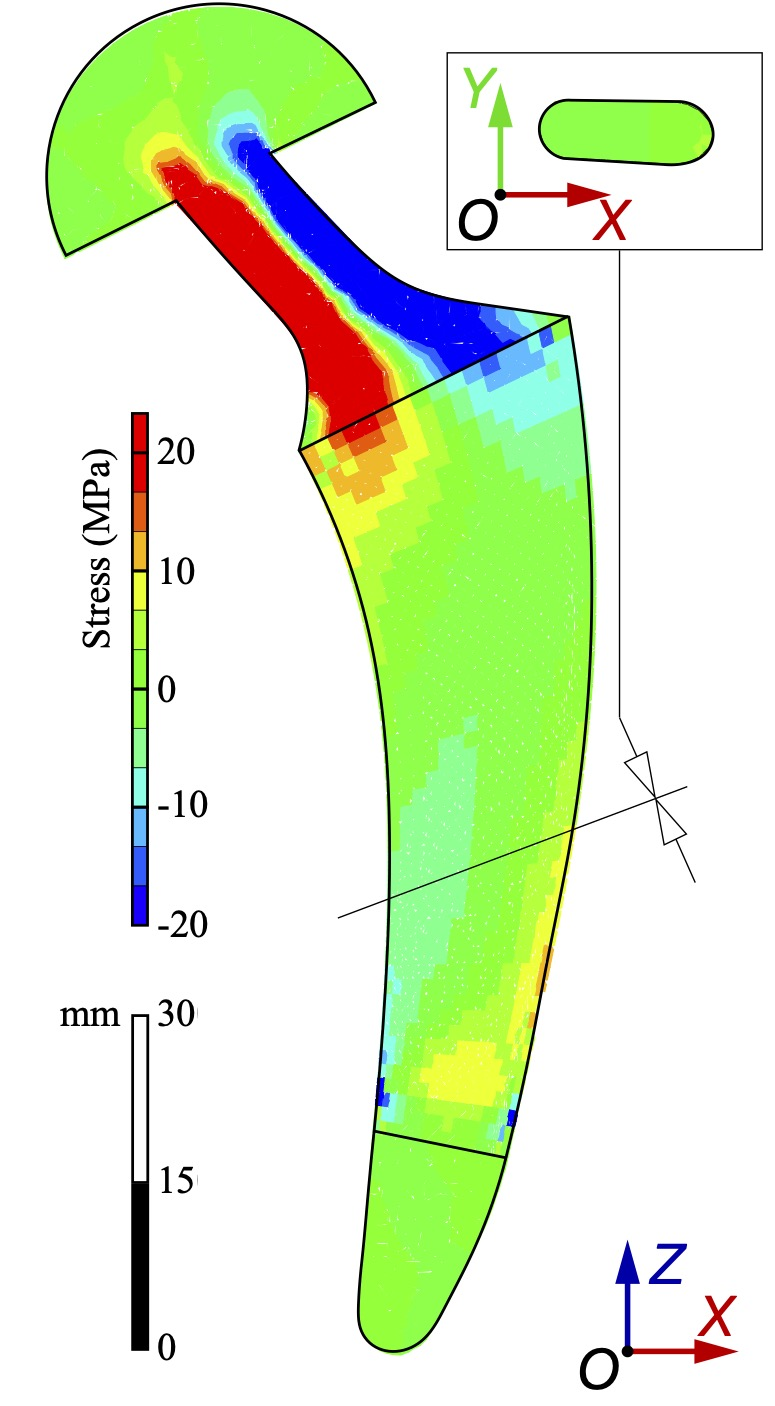
\includegraphics[width=4 cm]{fig/s13}}
\subfigure[]{
\label{s12}
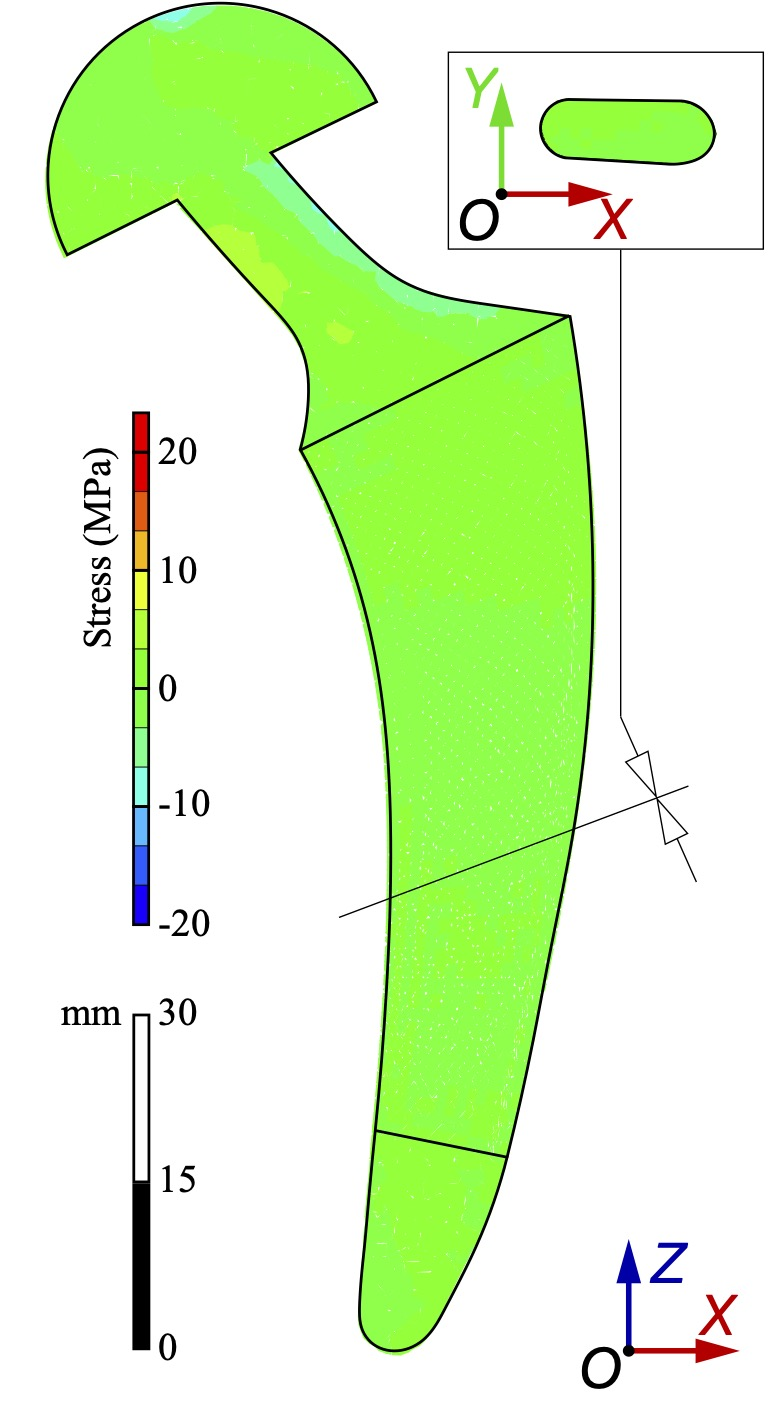
\includegraphics[width=4 cm]{fig/s12}}
\caption{Distribution of stress components in uniform-density lattice implant with 50\% overall relative density and isotropic microstructure: (a) $s_{11}$; (b) $s_{22}$; (c) $s_{33}$; (d) $s_{23}$; (e) $s_{13}$; (f) $s_{12}$.}
\label{component}
\end{figure}

\subsection{Bio-mechanical performance}

To make comparative analysis on optimization results, four implant products with different interior structure designs are selected as representative cases, which includes:\\

\begin{itemize}
\item {\bf Solid implant}:\\
Unit cells in the optimization domain are assigned with solid Ti$_6$Al$_4$V materials. The mechanical properties refers to Table~\ref{property_femur}.
\item {\bf Uniform-density isotropic lattice implant}:\\
Unit cells in the otpimization domain are assigned with 50\% unit cell relative density and isotropic anisotropy pattern. The mechanical properties refers to Table~\ref{property_femur}. 
\item {\bf Graded-density isotropic lattice implant}:\\
Unit cells in the otpimization domain are assigned with isotropic microstructures. The overall relative density of the implant is controlled to be 50\%. The mechanical properties of unit cells are calculated from the data-driven GP model.
\item {\bf Graded-density anisotropic lattice implant}:\\
Unit cells in the otpimization domain are assigned with anisotropic microstructures. The overall relative density of the implant is controlled to be 50\%. The mechanical properties of unit cells are calculated from the data-driven GP model.\\
\end{itemize}

Fig.~\ref{stress_implant} and Fig.~\ref{stress_femur} show the stress distribution condition in femoral implant and femoral head with different implant interior structure design. In the situation of fully-filled solid implant (Fig.~\ref{stress_solid}), high von Mises stress over 40 MPa is observed along the front and rear edge of optimization domain, while a stress trough down to 0 appears at the center of the implant. By replacing the solid finite elements with 50\% relative density isotropic unit cells (Fig.~\ref{stress_uniform}), the magnitudes of stress in implant domain are reduced by about 30\%. However, stress concentration still happens around the front and rear surfaces of implant, indicating high pressure transferred from surrounding bones. This problem is modified by assigned graded relative density to unit cells (Fig.~\ref{stress_isot}). In the upper half part of the implant, stress are shifted from surfaces to implant center and stress concentration on contacting surface are efficiently moderated. The best performance is achieved by graded-density implant with anisotropic lattice microstructures. By introducing unit cell anisotropy pattern as an extra design variable, the stress in implant is further decreased (Fig.~\ref{stress_anis}). For most areas besides the implant center, the magnitudes of von Mises is lower than 10 MPa, indicating an enhanced implant compliance.\\

\begin{figure}[htbp]
\centering
\subfigure[]{
\label{stress_solid}
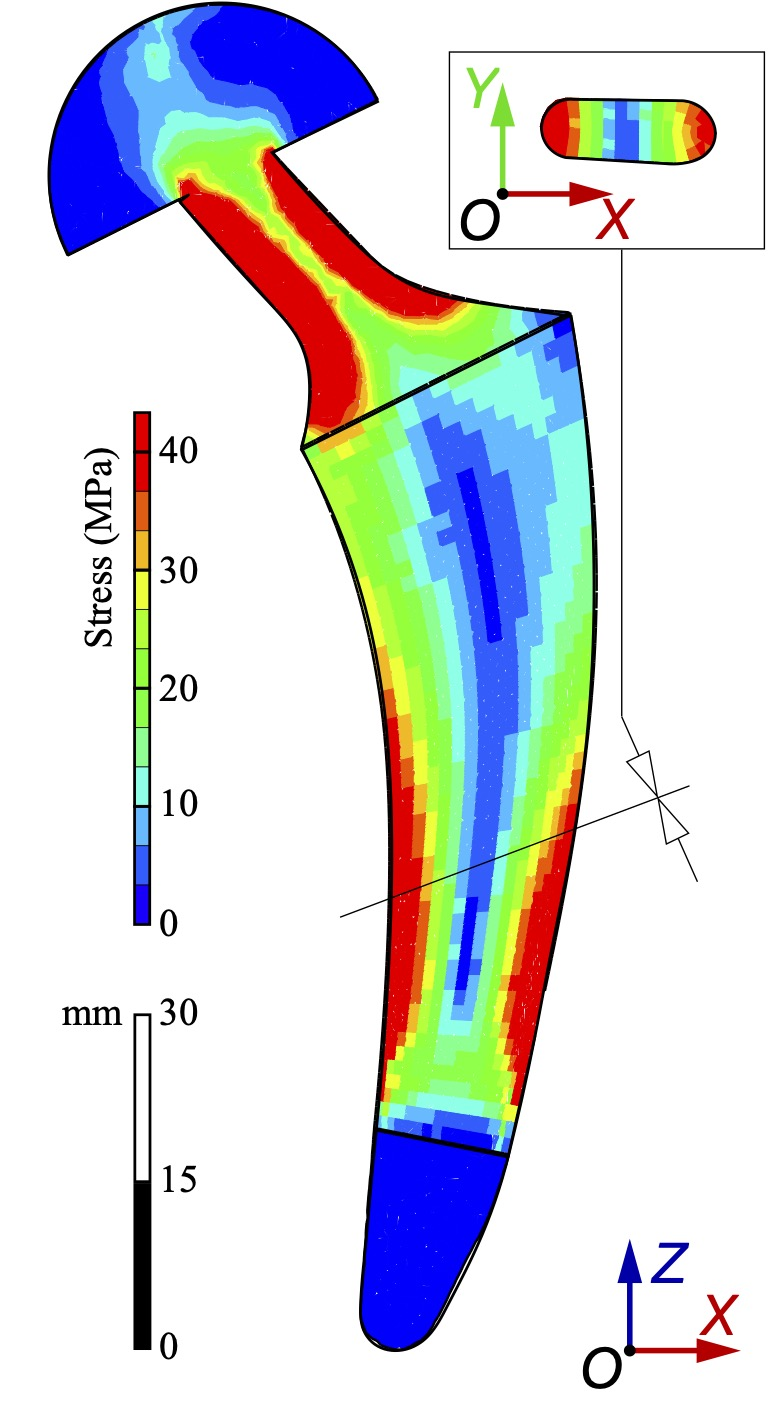
\includegraphics[width=4 cm]{fig/stress_solid}}
\subfigure[]{
\label{stress_uniform}
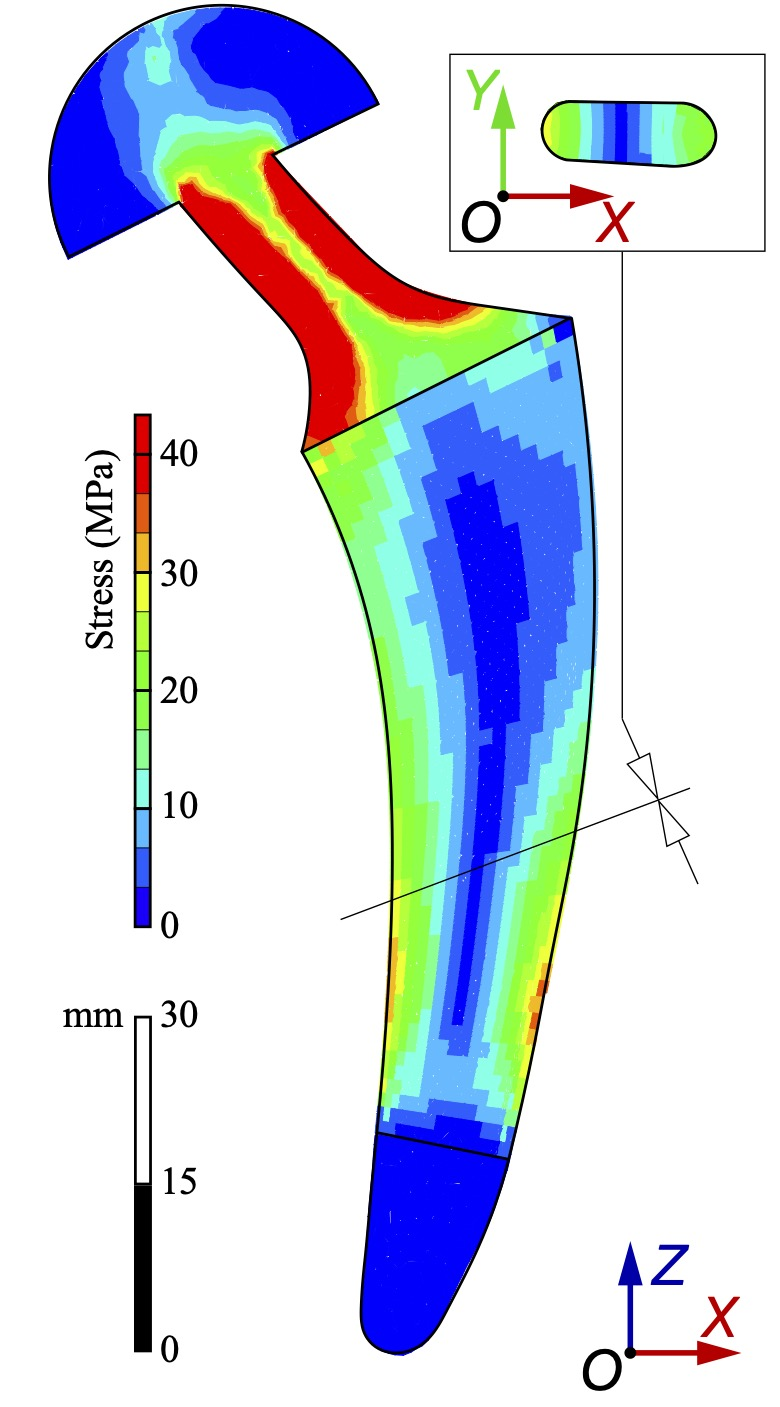
\includegraphics[width=4 cm]{fig/stress_uniform}}\\
\subfigure[]{
\label{stress_isot}
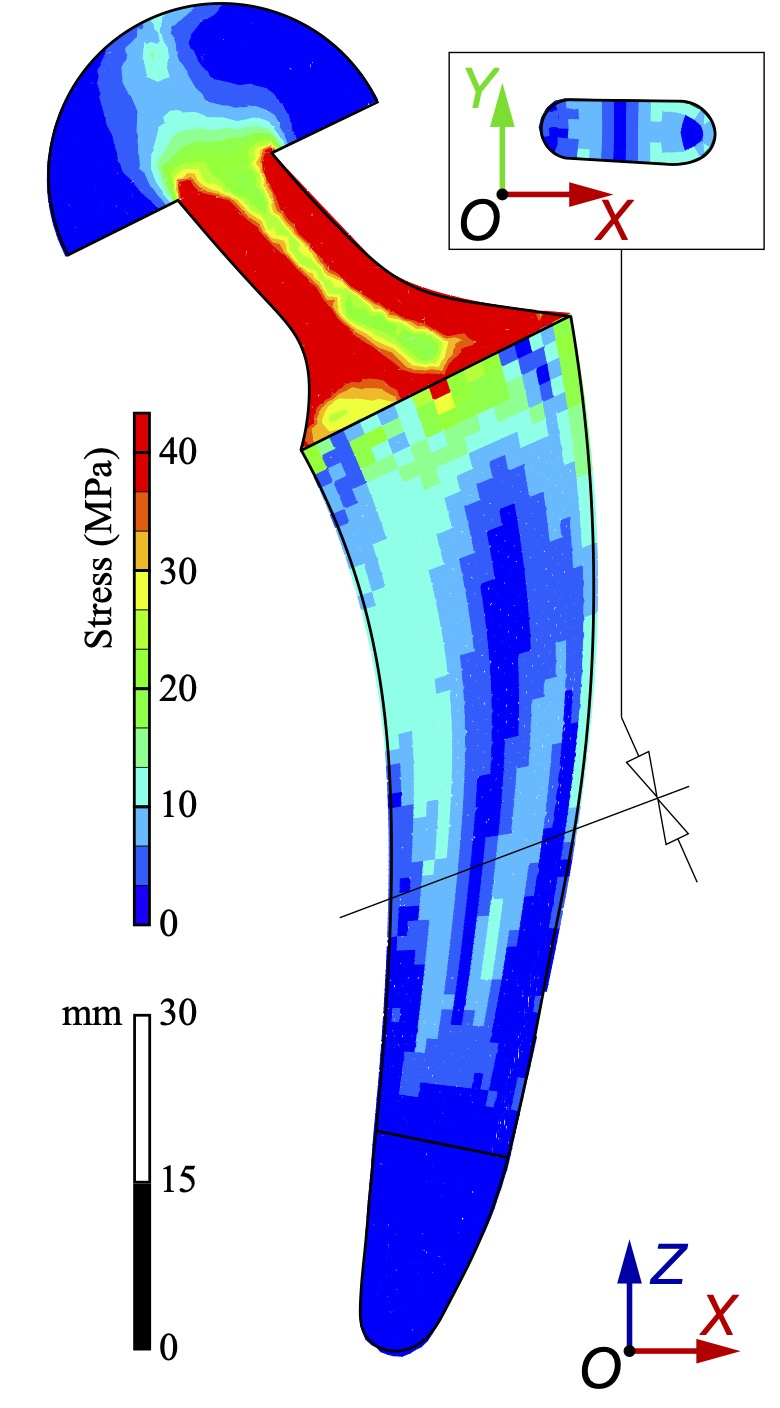
\includegraphics[width=4 cm]{fig/stress_isot}}
\subfigure[]{
\label{stress_anis}
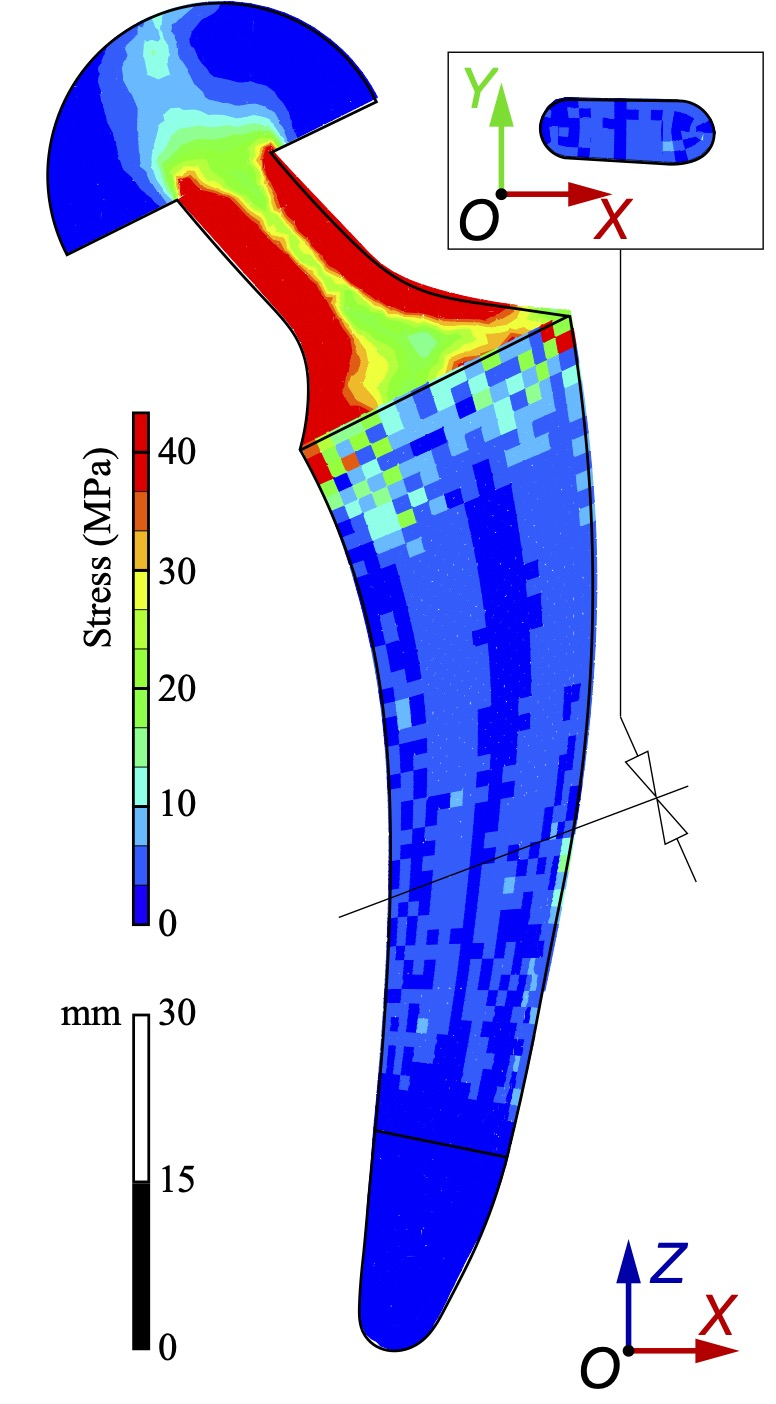
\includegraphics[width=4 cm]{fig/stress_anis}}
\caption{Distribution of von Mises stress in: (a) solid implant; (b) uniform-density isotropic lattice implant; (c) graded-density isotropic lattice implant; (d) graded-density anisotropic lattice implant.}
\label{stress_implant}
\end{figure}

\begin{figure}[htbp]
\centering
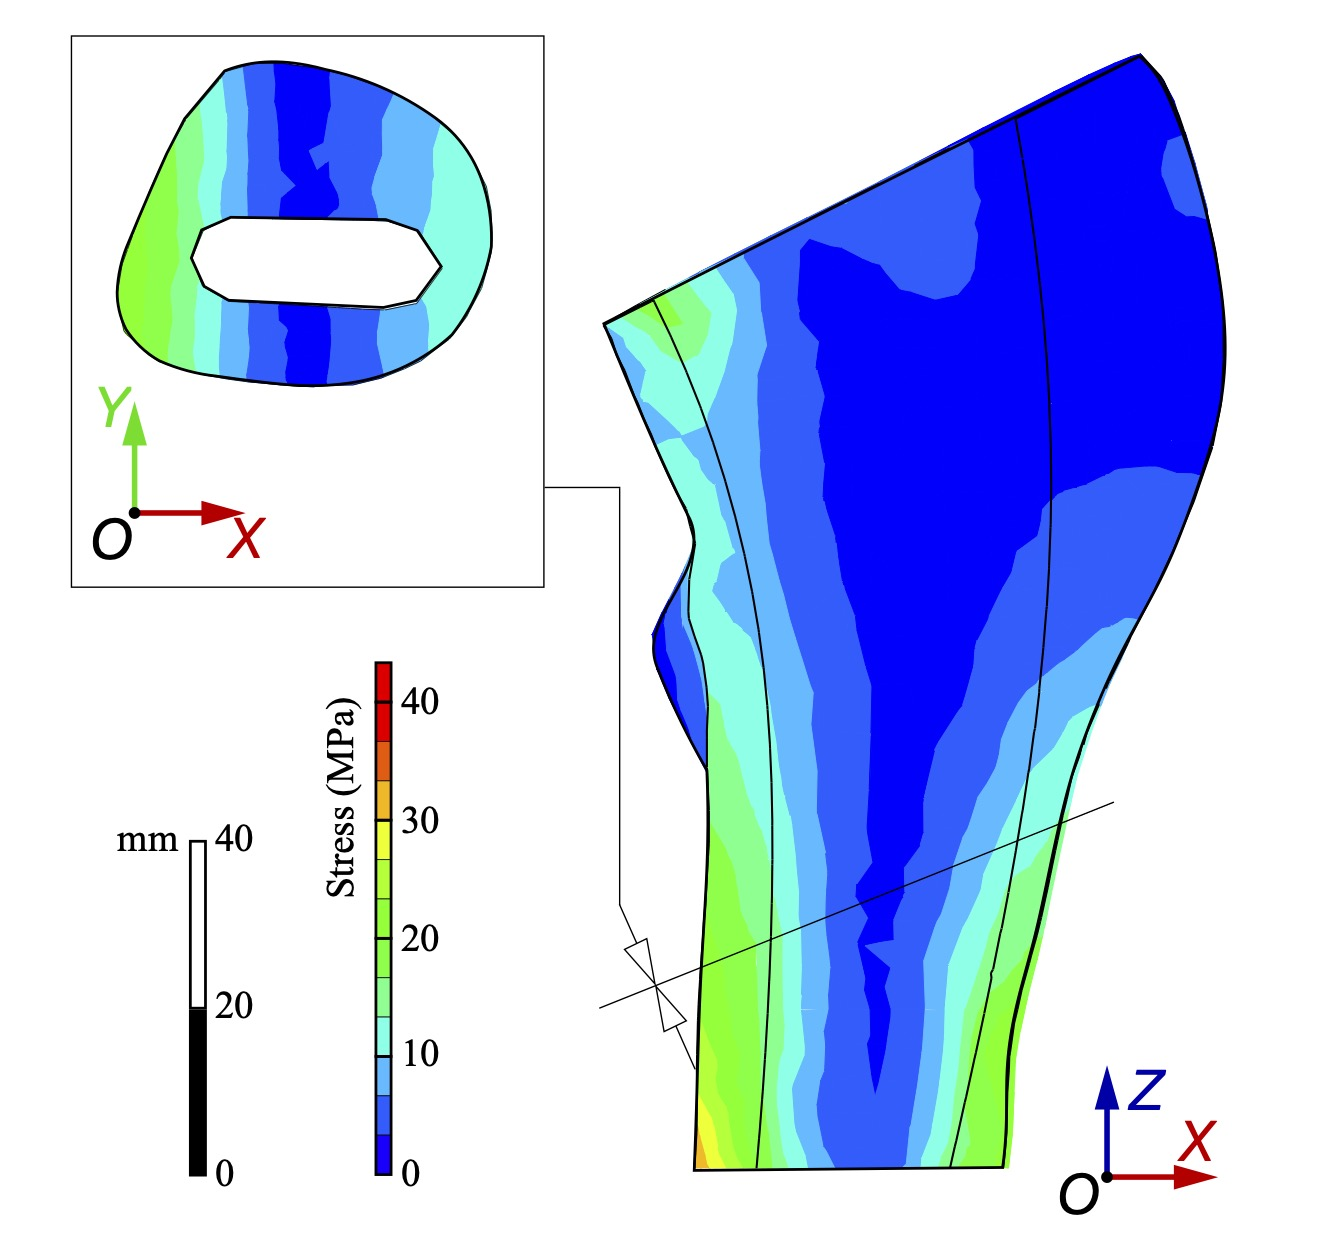
\includegraphics[width=10 cm]{fig/stress_fem_original}
\caption{Distribution of von Mises stress in preoperative femur head.}
\label{stress_fem_original}
\end{figure}

Loading pressures removed from implant are re-allocated to femur bone tissue. From Fig.~\ref{stress_fem_solid} to Fig.~\ref{stress_fem_anis}, stress nearby the bone-implant interface inside the femur head gradually increases, making the stress distribution closer to that in preoperative bone (Fig.~\ref{stress_fem_original}, removed bone tissue is not presented). The bone stress reduction caused by different implant designs are shown in Fig.~\ref{mbr_femur} to reflect the severity of bone resorption. The resorbed bone mass fraction caused by the four implants are 17.413\%, 3.483\%, 3.015\% and 1.827\% respectively. The stress shielding severity are 8.700\%, 4.387\%, 2.847\% and 1.661\% respectively. Fig.~\ref{mbr_fem_solid} reveals the severe bone degeneration situation in femur with solid implant. Most bone tissues are in red color (over 30\% stress reduction), indicating a high possibility of pathological osteoporosis. By adopting uniform-density lattice interior design (Fig.~\ref{mbr_fem_uniform}), the degeneration zone at posterior of epiphysis proximal shrinks but that at anterior side is still considerable until the relative density among implant domain is redistributed (Fig.~\ref{mbr_fem_isot}). Graded-density implant with anisotropy microstructures further moderates this problem(Fig.~\ref{mbr_fem_anis}). Limited degeneration zones are observed in femur proximal. For most areas in femur domain, the stress reduction is less than 12.5\%, indicating a notably low risk of postoperative osteoporosis and implantation failure.\\


\begin{figure}[htbp]
\centering
\subfigure[]{
\label{stress_fem_solid}
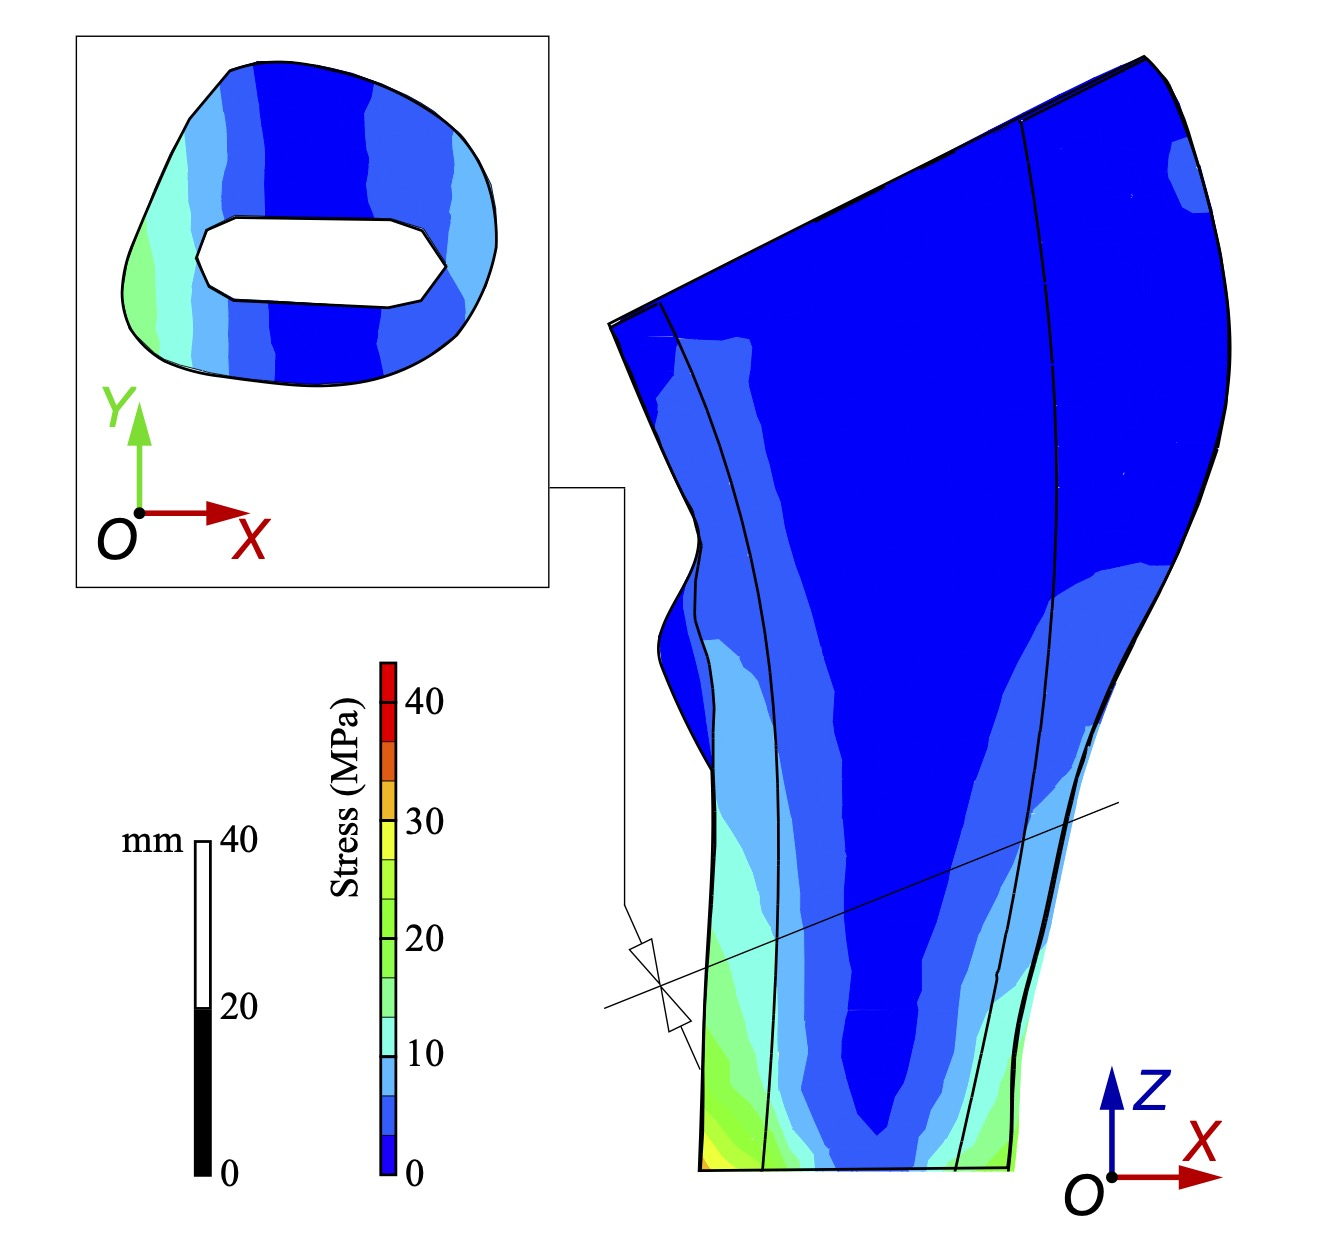
\includegraphics[width=7.3 cm]{fig/stress_fem_solid}}
\subfigure[]{
\label{stress_fem_uniform}
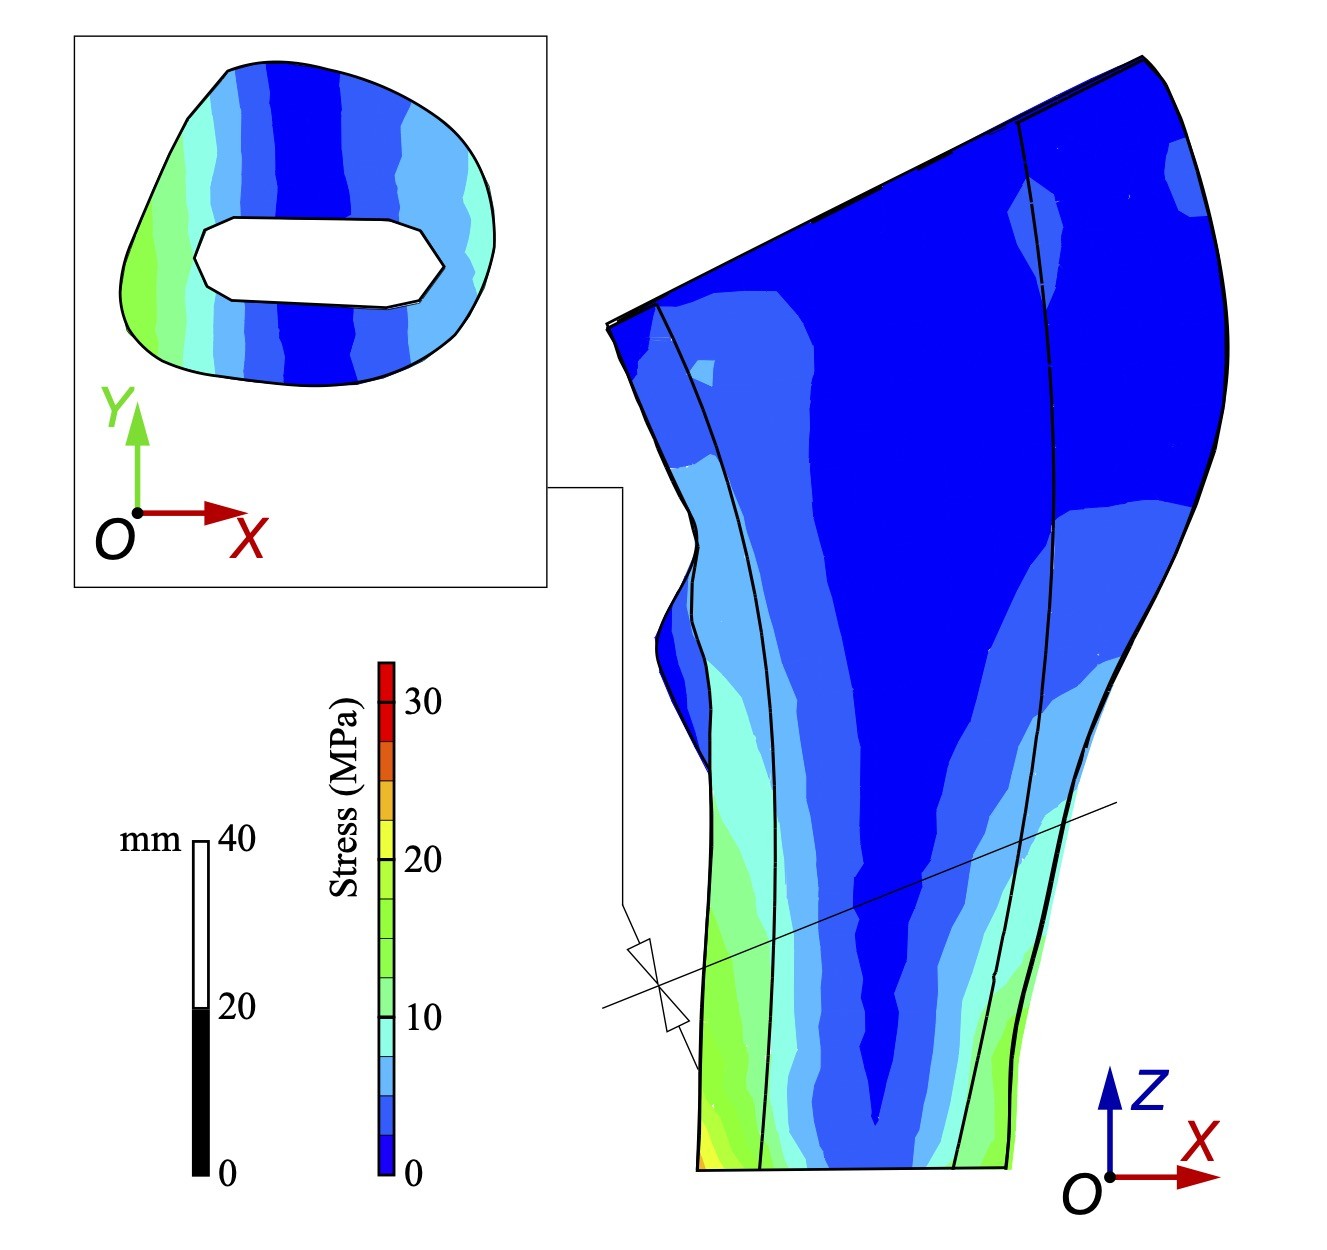
\includegraphics[width=7.3 cm]{fig/stress_fem_uniform}}
\subfigure[]{
\label{stress_fem_isot}
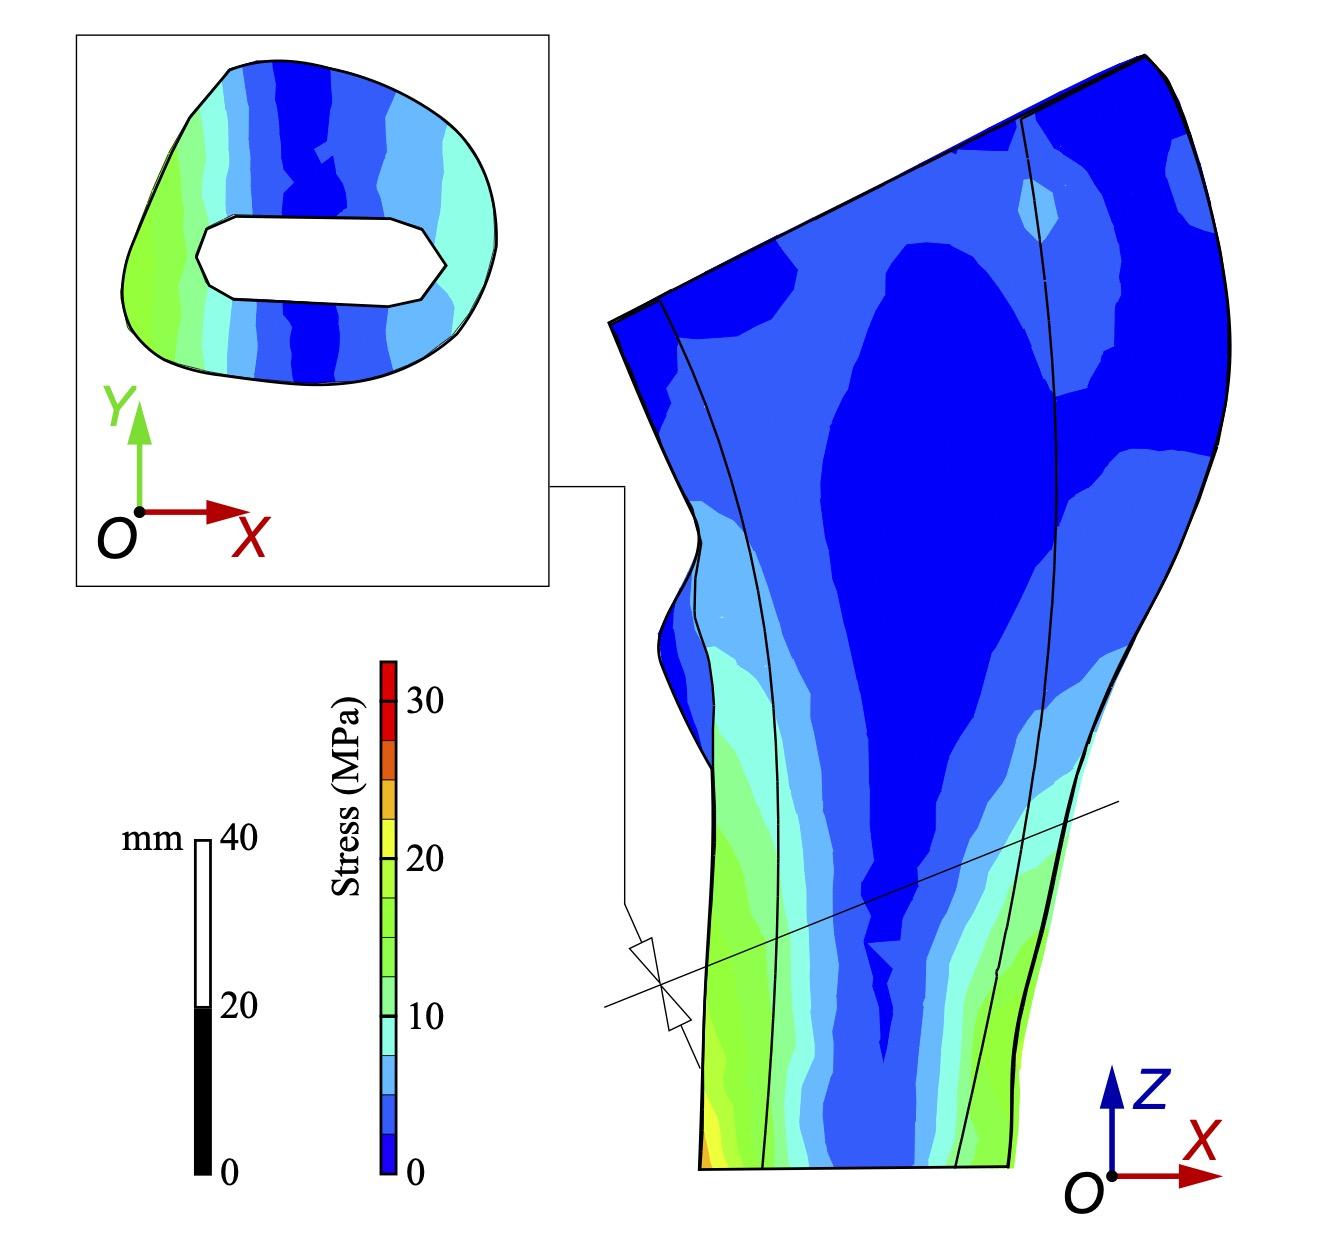
\includegraphics[width=7.3 cm]{fig/stress_fem_isot}}
\subfigure[]{
\label{stress_fem_anis}
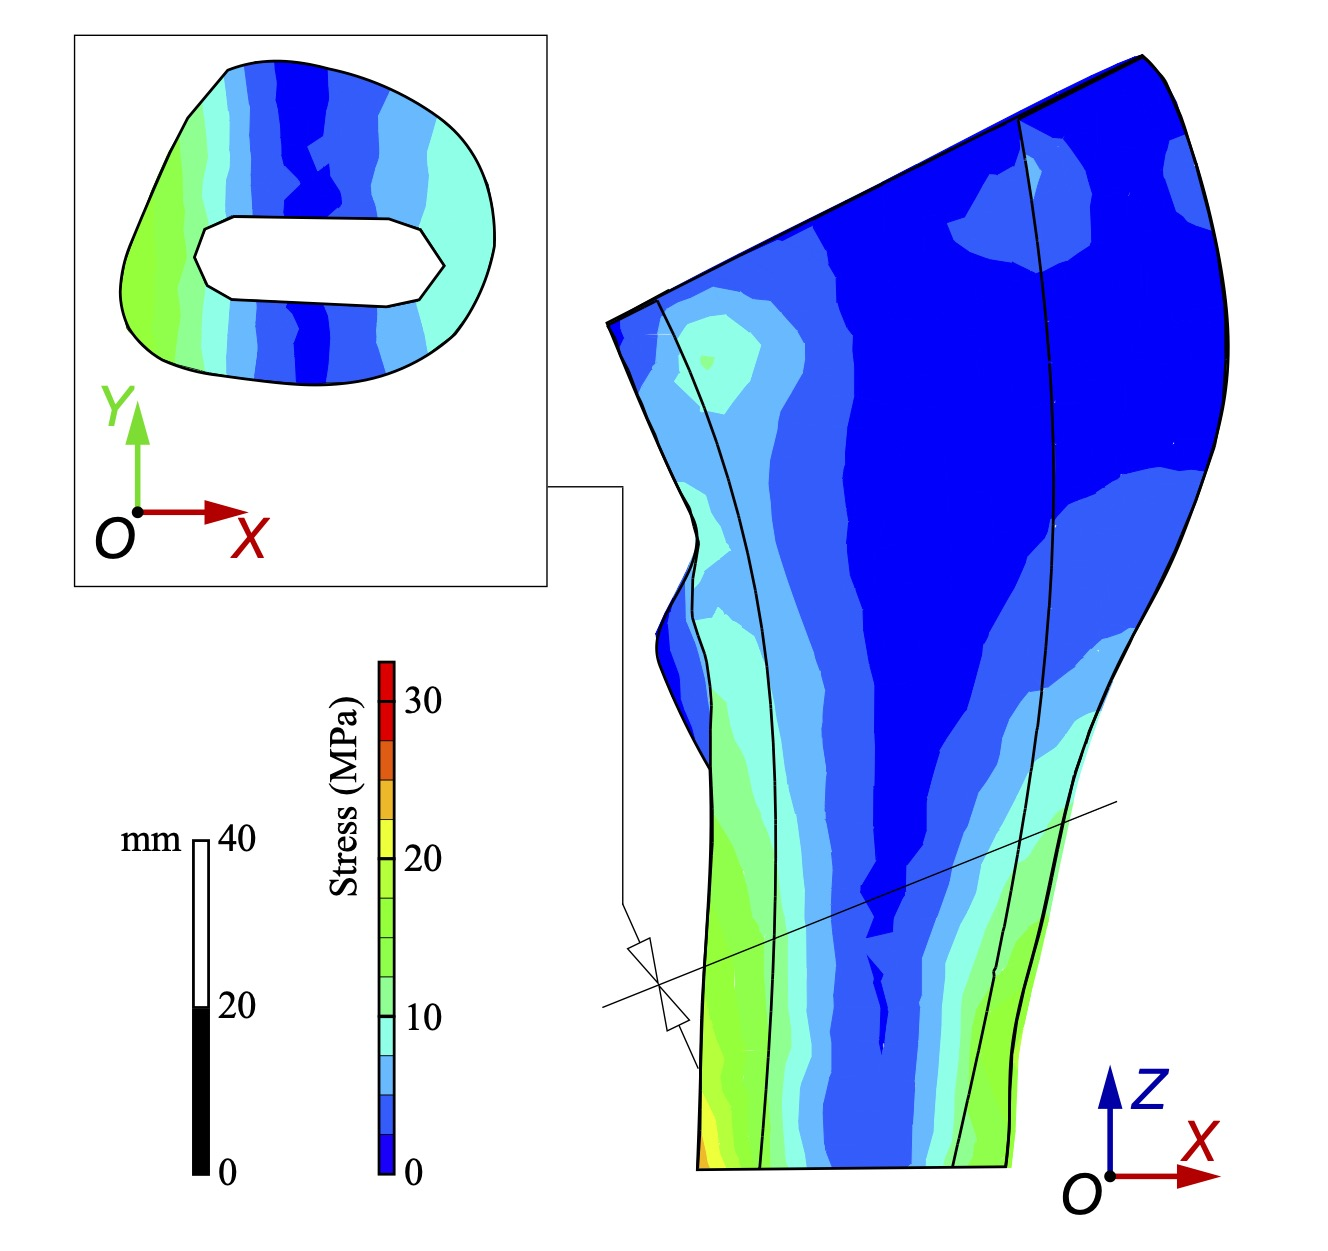
\includegraphics[width=7.3 cm]{fig/stress_fem_anis}}
\caption{Distribution of von Mises stress in femur head with: (a) solid implant; (b) uniform-density isotropic lattice implant; (c) graded-density isotropic lattice implant; (d) graded-density anisotropic lattice implant.}
\label{stress_femur}
\end{figure}

\begin{figure}[htbp]
\centering
\subfigure[]{
\label{mbr_fem_solid}
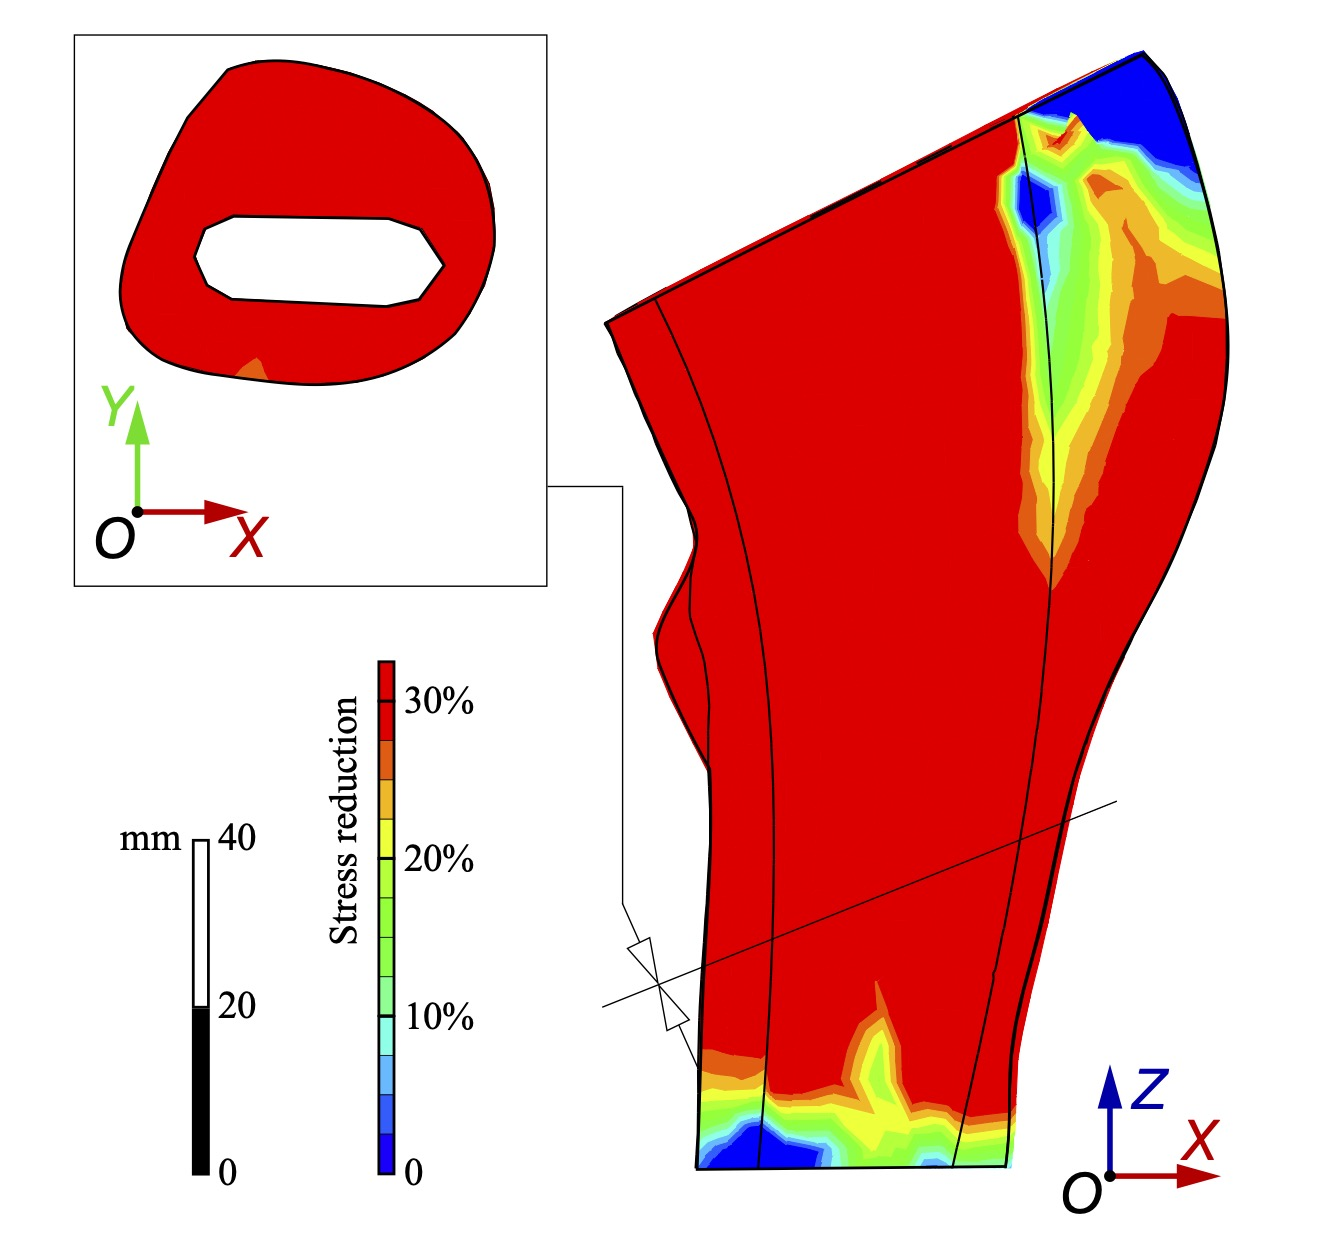
\includegraphics[width=7.3 cm]{fig/mbr_fem_solid}}
\subfigure[]{
\label{mbr_fem_uniform}
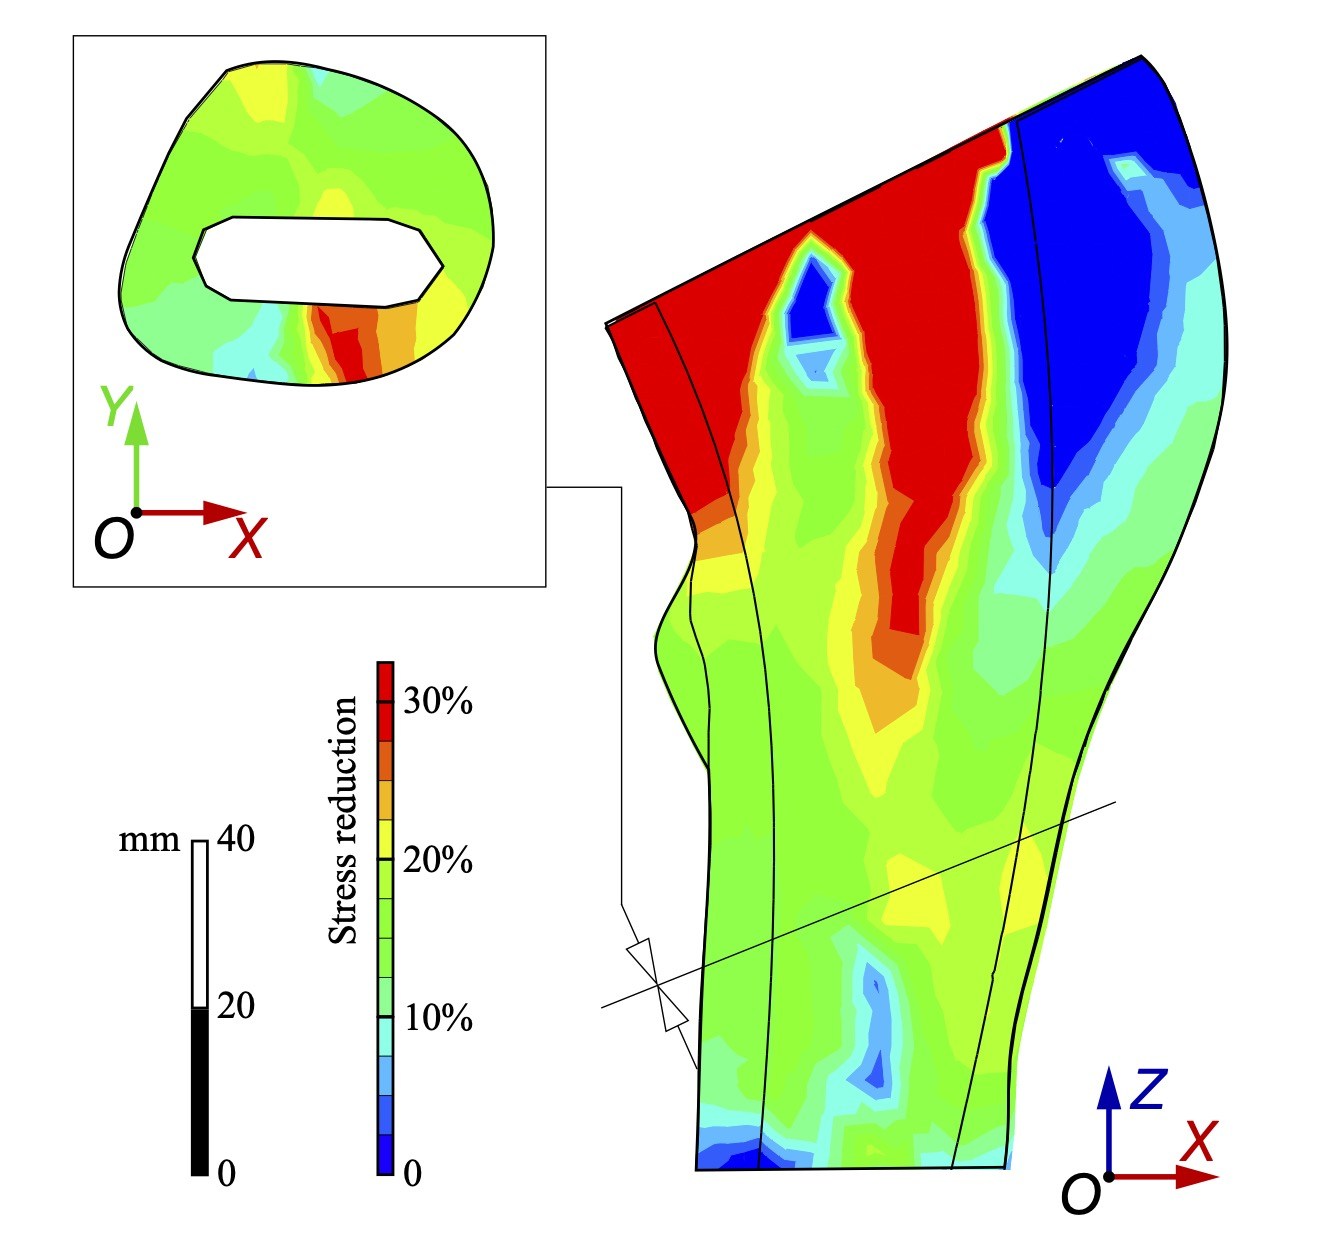
\includegraphics[width=7.3 cm]{fig/mbr_fem_uniform}}
\subfigure[]{
\label{mbr_fem_isot}
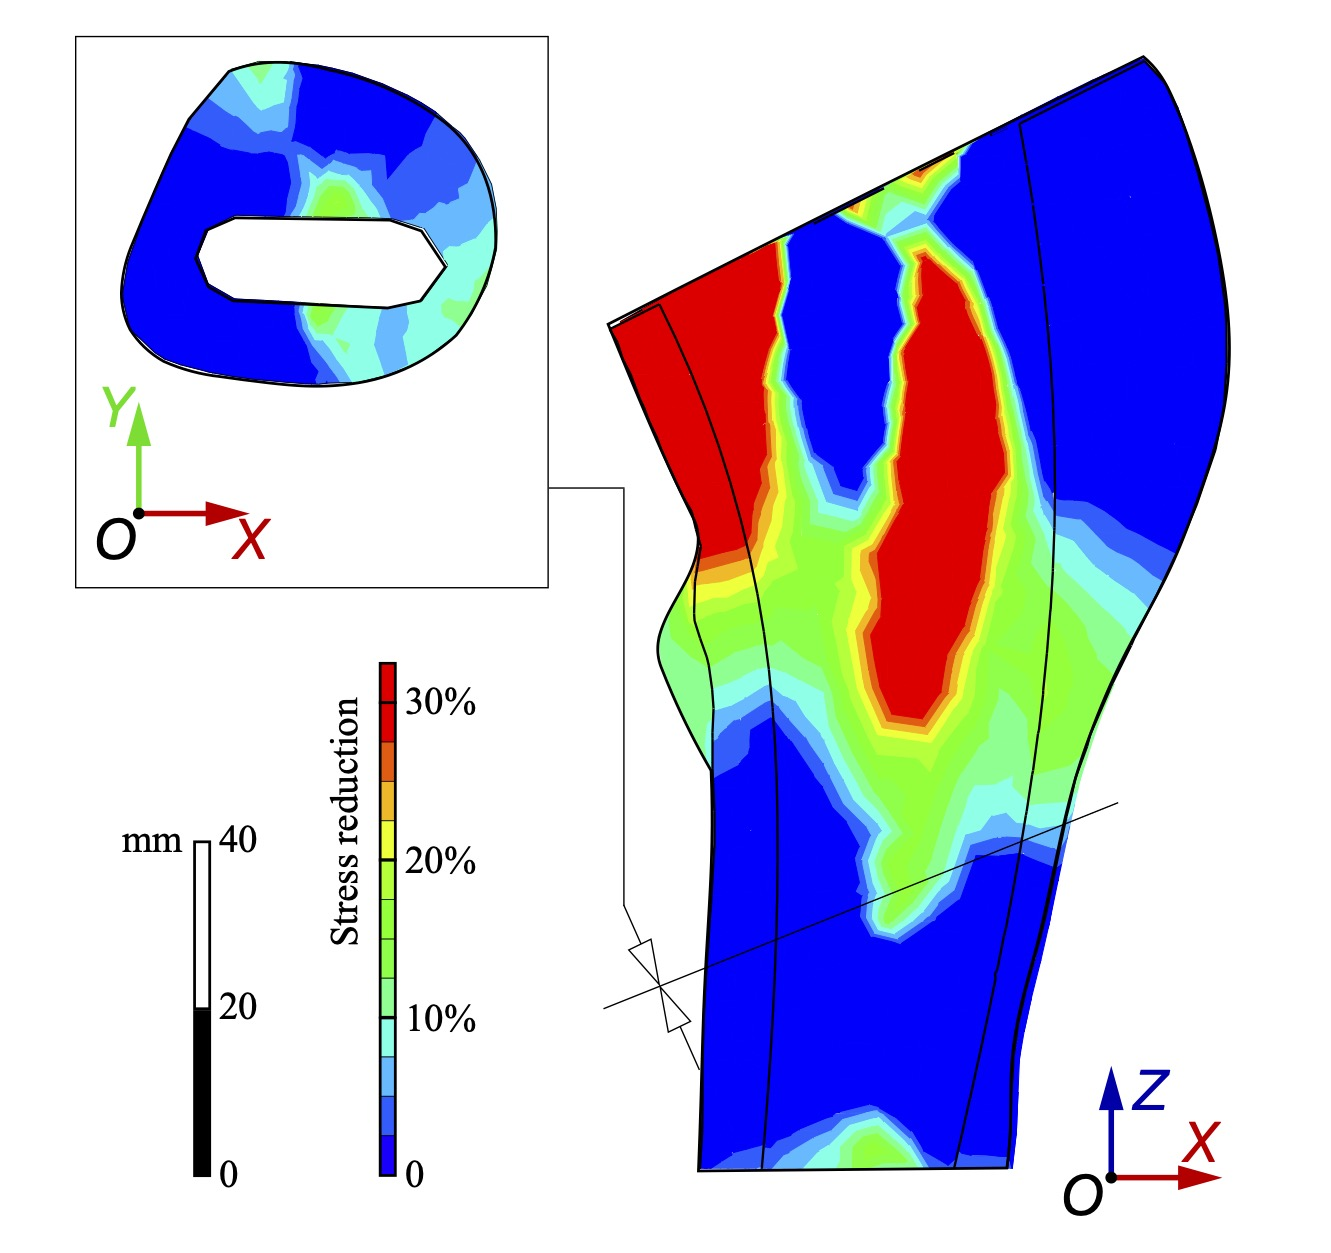
\includegraphics[width=7.3 cm]{fig/mbr_fem_isot}}
\subfigure[]{
\label{mbr_fem_anis}
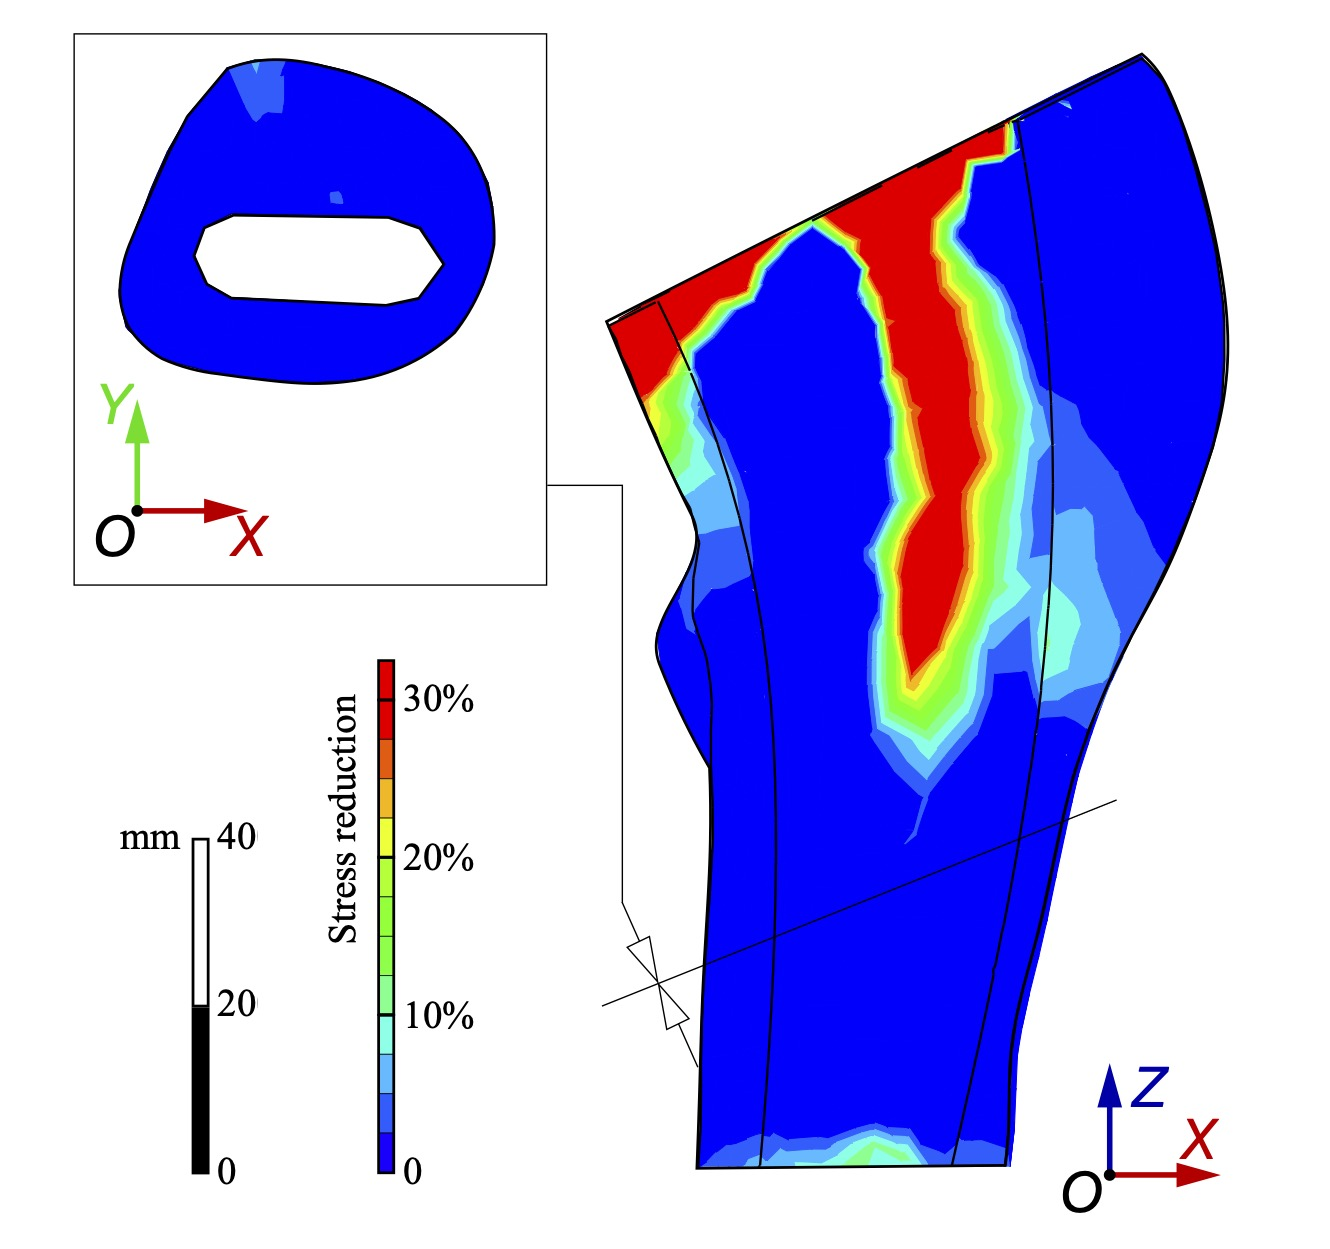
\includegraphics[width=7.3 cm]{fig/mbr_fem_anis}}
\caption{Distribution of postoperative bone stress reduction in femur head with: (a) solid implant; (b) uniform-density isotropic lattice implant; (c) graded-density isotropic lattice implant; (d) graded-density anisotropic lattice implant.}
\label{mbr_femur}
\end{figure}

\section{Conclusion}
\label{femur_conc}

In this chapter, an optimization design framework is established based on MMA algorithm to customize the relative density distribution and anisotropy pattern arrangement in lattice femoral implant according to actual stress condition in patient's body. The constitutive relationship of anisotropic lattice unit cells are homogenized based on the data-driven GP model introduced in Chapter~\ref{gauss}.\\

The optimization framework takes maximum implant compliance as design target, so that concentrated loads in metallic implant are transferred to proximal femur and bone degeneration caused by stress shielding is hence moderated. Constraint conditions includes structural failure criteria, bone growth stimulation, additive manufacturing capability are applied to satisfy clinical and fabrication requirement.\\

The efficacy of stress shielding moderation is quantitatively evaluated by resorbed bone mass fraction in post-implantation femur. Compared to solid implant, uniform-density isotropic implant and graded-density isotropic implant, the optimized graded-density anisotropic implant reduces the resorbed bone mass by 89.5\%, 47.5\% and 39.4\%, indicating its high practical value in total hip arthroplasty clinical treatment.\\


%========================================
%========================================
%========================================


\chapter{Topology optimization of lattice spinal cage under differentiated bio-mechanical loading conditions}
\label{spine}

In this chapter, the optimization design framework used in Chapter~\ref{femur} is applied to the design of lattice spinal cages with different body load eccentricities (non-eccentric, flexion, extension and lateral bending). 
The spinal cages are composed by isotropic lattice microstructures with varied relative densities distributions. Differentiated optimal cage interior lattice designs are obtained against assigned loading conditions.\\

\section{Finite element model}
\label{spine_mode}

\subsection{Geometry and meshing}

The geometric models (Fig.~\ref{fsu_model}) used in in this chapter include a complete functional spine unit (FSU), containing one L3 vertebra, one L4 vertebrae and a intervertebral spinal cage, reflecting the spine clinical situation after lumbar inter-body fusion (LIF) treatment. The lower endplate of L3 and upper endplate of L4 are polished to represent the removal of cartilaginous components during treatment\cite{latif2022vertebral}. As a proof-of-concept study, homogeneous linear mechanical property is assigned to vertebrae components. For the spinal disc, the influence of annulus fibrosus and the nucleus pulposus are taken into consideration and a homogenized elastic model is adopted. The shape of spinal cage takes reference to a common trapezoidal cage configuration used during anterior LIF procedures. Compared to other cage designs, the trapezoidal shape maximizes contacting surface area between vertebrae and cage~\cite{yoo2019interbody}, providing higher flexibility to the optimization design interior lattice microstructures. Similar to femoral implant in Section~\ref{femur_mode}, $\text{Ti}_6\text{Al}_4\text{V}$ is selected as the base material of spinal cage. Mechanical properties of 50\% porosity isotropic lattice microstructures is assigned at first iteration step. Details of material properties are shown in Table~\ref{property_spine}~\cite{lu2013strain},~\cite{perie2005confined}.\\

\begin{table}[htbp]
\centering
\caption{Mechanical properties of materials used in LIF finite element modeling.}
\begin{tabular}{lrrr}
\hline\hline
Material & $\rho_m$ (kg/m\textsuperscript{3}) & $E$ (GPa) & $\nu$\\
\hline
Homogeneous bone & 1800 & 5.0 & 0.31\\
Spinal disc & 1200 & 0.75 & 0.30\\
$\text{Ti}_6\text{Al}_4\text{V}$ (solid) & 4512 & 119.0 & 0.31\\
$\text{Ti}_6\text{Al}_4\text{V}$ (50\%, isotropic)& 2256 & 28.4 & 0.27\\
Rubber gasket & 1522 & 11.25 & 0.45\\
\hline\hline
\end{tabular}
\label{property_spine}
\end{table}

\begin{figure}[htbp]
\centering
\subfigure[]{
\label{fsu_pers}
\includegraphics[width=7.3 cm]{fig/fsu_pers}}
\subfigure[]{
\label{fsu_front}
\includegraphics[width=7.3 cm]{fig/fsu_front}}
\subfigure[]{
\label{fsu_side}
\includegraphics[width=7.3 cm]{fig/fsu_side}}
\subfigure[]{
\label{fsu_plane}
\includegraphics[width=7.3 cm]{fig/fsu_plane}}
\caption{Geometric models of FSU: (a) perspective view; (b) front view; (c) side view; (d) plane view.}
\label{fsu_model}
\end{figure}

The FSU components, including spinal cage, L3 and L4 vertebrae are meshed with linear tetrahedron finite elements (Fig.~\ref{fsu_vet}). Aspect ratio and volume inhomogeneity are limited to be lower than 0.9 to avoid element distortion. The side length of the finite element is 2 mm. the surface mesh on vertebrae-cage interface are kept consistence to avoid finite element calculation error.\\

The entire the spinal cage is defined as the optimization domain. As an application of multi-scale computation method, during the iteration process, each finite element is assigned with a specific relative density and mechanical properties, so that to represent a unique lattice tetrahedron microstructure.\\

\begin{figure}[htbp]
\centering
\subfigure[]{
\label{fsu_vet}
\includegraphics[width=8 cm]{fig/fsu_vet}}
\subfigure[]{
\label{fsu_tet}
\includegraphics[width=8 cm]{fig/fsu_tet}}
\caption{Finite element models of FSU: (a) vertebrae with tetrahedron mesh; (b) spinal cage with tetrahedron mesh.}
\label{fsu_mesh}
\end{figure}

\subsection{Boundary conditions}

The L3-L4 FSU is placed between two loading plates to simulate the body load condition in patients' bodies (Fig.~\ref{plate_gasket}). Between the rigid plates and vertebra endplates, a rubber gasket is inserted, so that the loads are transferred evenly among the endplate surfaces and avoid local stress concentration. Material properties of rubber gasket in recorded in Table~\ref{property_spine}.\\

\begin{figure}[htbp]
\centering
\includegraphics[width=10 cm]{fig/plate_gasket}
\caption{Set-up of loading plate and rubber gasket on FSU for loading transmission.}
\label{plate_gasket}
\end{figure}

The rigid part of lower loading plates in all cases are fixed in both translational and rotational directions. The facets of articular process are bounded. A vertical load in 1000 N magnitude is applied to the upper loading plate, to represent the extreme instantaneous body load generated during daily activities. Four loading eccentricity conditions, including ``non-eccentric'', ``flexion'', ``extension'' and ``lateral bending''~\cite{brandolini2014experimental}, are shown in Fig.~\ref{spine_loading}. In non-eccentric condition, the loading position locates at the gravity center of the vertebra endplates. In flexion and extension conditions, the loading position is offset by 20\% of the antero-posterior depth along anterior and posterior directions respectively. In lateral bending condition, the loading position is offset by 20\% of the coronal width along lateral direction. The positions of the loadings are shown in Table~\ref{loading_position}.\\

\begin{figure}[htbp]
\centering
\subfigure[]{
\label{loading_noneccentric}
\includegraphics[width=7.3 cm]{fig/loading_noneccentric}}
\subfigure[]{
\label{loading_flexion}
\includegraphics[width=7.3 cm]{fig/loading_flexion}}
\subfigure[]{
\label{loading_extension}
\includegraphics[width=7.3 cm]{fig/loading_extension}}
\subfigure[]{
\label{loading_bending}
\includegraphics[width=7.3 cm]{fig/loading_bending}}
\caption{Different spine loading conditions: (a) non-eccentric; (b) flexion; (c) extension; (d) lateral bending.}
\label{spine_loading}
\end{figure}

\begin{table}[htbp]
\centering
\caption{Location of applied loading on FSU.}
\begin{tabular}{lrr}
\hline\hline
Loading case & $x$-coordinate (mm) & $z$-coordinate (mm)\\
\hline
Non-eccentric loading & 0 & 0\\
Flexion loading& -8.12 & 0\\
Extension loading & 8.12 & 0\\
Lateral bending & 0 & 12.04\\
\hline\hline
\end{tabular}
\label{loading_position}
\end{table}


\subsection{Mechanical property homogenization}

The multi-scale simulation method is adopted in finite element analysis to reduce the computational cost caused by complicated lattice interior structure. Each finite element is assigned with homogenized mechanical properties to represent an lattice microstructure in practice.\\

Tetrahedron-based lattice cube (Fig.~\ref{tet_cube}) with uniform in-cell strut radii is established to compute the analytical expression of effective mechanical properties against cube relative density. Similar to Section~\ref{gauss_data}, the stiffness components and failure strengths of microstructures are calculated based on asymptotic homogenization (AH) method. The analytical expressions of the mechanical properties refer to previous literatures~\cite{wang2018hip}.

\begin{figure}[htbp]
\centering
\subfigure[]{
\label{tet_cube_30}
\includegraphics[width=4.7 cm]{fig/tet_cube_30}}
\subfigure[]{
\label{tet_cube_60}
\includegraphics[width=4.7 cm]{fig/tet_cube_60}}
\subfigure[]{
\label{tet_cube_90}
\includegraphics[width=4.7 cm]{fig/tet_cube_90}}
\caption{Tetrahedron-based lattice cube in: (a) 30\% relative density; (b) 60\% relative density; (c) 90\% relative density.} 
\label{tet_cube}
\end{figure}


\section{Optimization framework}

\subsection{Objective function}

Since the stiffness of titanium alloy is much higher than intervertebral disc, after spinal cage replacement, the uneven pressure distribution on endplate contacting surface aggravates. Compared to high-pressure zones in pre-implantation vertebrae, low-pressure zones suffer higher stress reduction, and subsequently more severe bone degeneration. As a countermeasure, the local stiffness in spinal cage nearby high-stress zones can reduced by removing basis materials from the lattice unit cells, so as to decrease the loading resistance and generate higher pressure in other contacting zones.\\

Similar to Section~\ref{femur_opti}, maximum compliance is selected as the optimization design target. As observed during finite element simulation, higher stress in vertebrae leading to higher strain energy in spinal cage counterpart. Therefore in order to increase the global compliance among optimization domain, local stiffness at high pressure zones is to be reduced, which fits the above-mentioned stress redistribution ideology. The mathematical expression is:
\begin{equation}
U = \sum_{i=1}^N \bm{\varepsilon}_i^T\bm{C}_i\bm{\varepsilon}_i
\label{4-2-T1}
\end{equation}

Where $\bm{\varepsilon}$ is element strain tensor, $\bm{C}$ is element constitutive matrix and $N$ is the amount of elements in optimization domain.\\

\subsection{Constraint conditions}

The constraint conditions involved in femoral implant optimization design (Section~\ref{femur_opti}) are applicable to the design of lattice spinal cages.\\

\subsubsection{Structural failure criteria}

The Tsai-wu criteria~\cite{tsai1971general} should be satisfied during the design process to avoid failure of lattice microstructures:
\begin{equation}
\text{SF} = 1 / (\sum_{i=1}^{3}F_{ii}s_{ii}^2 + F_{44}s_{23}^2 + F_{55}s_{13}^2 + F_{66}s_{12}^2)  \geq 1
\label{4-2-2}
\end{equation}

Definition of Tsai-wu parameters $\bm{F}$ and stress tensor $\bm{s}$ refers to Equation~\ref{2-1-20} and Equation~\ref{3-2-3}.\\

\subsubsection{Bone growth stimulation and AM capability}

The diameter of pore on the contacting surface between vertebrae and spinal cage endplates should be 50 to 800 {\textmu}m~\cite{harrysson2008direct}. The diameter of lattice struts should be higher than 200 {\textmu}m to guarantee its printability with additive manufacturing technique~\cite{de2013bone}. The two constraints are determined before iteration process and are applied in the form of relative density design range in each unit cell.\\ 


\subsubsection{Material removal fraction}

The global material fraction $\tilde{\rho}$ of spinal cage is required to be within 2\% difference compared to the desired global material fraction $\hat{\rho}$:
\begin{equation}
0.98\hat{\rho} \leq \tilde{\rho} \leq 1.02\hat{\rho}\\
\label{4-3-2}
\end{equation}

Definition of global material fraction $\tilde{\rho}$ refers to Equation~\ref{3-3-1}.\\



\subsection{Optimization algorithm}

The optimization algorithm adopted in this chapter is similar to the MMA algorithm used in Section~\ref{femur_opti}. The design variables are relative densities of all lattice cells in optimization domain. Bone ingrowth stimulation requirement and manufacturing capability constraints are represented by limitations on the range of unit cell relative densities while the failure criteria of cells are converted to constraint functions. The mathematical form is
\begin{equation}
\begin{array}{llll}
\text{maximise} & U(\{\rho\})\\
\text{subject to} & 1/(\text{SF}_i) \leq 1 & \text{for} & i = 1, 2,\cdots N\\
& -\tilde{\rho} \leq -0.98\hat{\rho}\\
& \tilde{\rho} \leq 1.02\hat{\rho}\\
& \rho_i^- \leq \rho_{i} \leq \rho_i^+ & \text{for} & i = 1, 2,\cdots N\\
\end{array}
\label{4-4-T1}
\end{equation}

Where $\{\rho\}\in\mathbb{R}_+^{N}$ is the relative density of unit cells in optimization domain, $\{\rho^-\}\in\mathbb{R}_+^N$ and $\{\rho^+\}\in\mathbb{R}_+^N$ are lower and upper bounds of unit cell relative density in optimization domain.\\

The termination of optimization iteration process follows the same criteria stated in Equation~\ref{3-4-7}, Section~\ref{femur_opti}.\\

\subsection{Sensitivity analysis}

Similar to Section~\ref{femur_opti}, the gradients of spinal cage global compliance, unit cell safety factors and global material fraction against unit cell relative densities are required to complete MMA optimization. For MMA algorithm with relative density and design variables, the gradients of global compliance is calculated as:
\begin{equation}
\frac{\partial U}{\partial \rho_i} \doteq -\frac{\bm{\varepsilon}_i^T[\bm{C}_i(\rho_i + \Delta \rho_i^+) - \bm{C}_i(\rho_i - \Delta \rho_i^-)]\bm{\varepsilon}_i}{\Delta \rho_i^- + \Delta \rho_i^+}
\label{4-4-T4}
\end{equation}

The gradient of Tsai-Wu safety factor in each finite element is:
\begin{equation}
\frac{\partial (1/\text{SF}_i)}{\partial \rho_i} \doteq \frac{\text{SF}_i(\rho_i - \Delta \rho_i^-) - \text{SF}_i(\rho_i + \Delta \rho_i^+)}{(\Delta \rho_i^- + \Delta \rho_i^+) \text{SF}_i(\rho_i + \Delta \rho_i^+) \text{SF}_i(\rho_i - \Delta \rho_i^-)}
\label{4-4-T5}
\end{equation}

The gradient of global material faction in spinal cage against unit cell relative density is:
\begin{equation}
\frac{\partial \tilde{\rho}}{\partial \rho_i} \doteq \frac{V_i (\Delta \rho_i^++ \Delta \rho_i^-)}{\sum_{j=1}^N V_j}
\label{4-4-T6}
\end{equation}


For all cases, the finite increment and decrement of relative density for linear approximation are defined as:
\begin{equation}
\left\{
\begin{array}{l}
\Delta \rho_i^- = \min\{0.005,~\rho_i\}\\
\Delta \rho_i^+ = \min\{0.005,~1 - \rho_i\}\\
\end{array}
\right.
\label{4-4-T10}
\end{equation}


\section{Performance evaluation}

The bio-mechanical performance of optimized spinal cages in post-operative FSU are evaluated by resorbed bone mass fraction and stress shielding intensity. Bone resorption is considered to happen in vertebra finite element when the reduction of stress is higher than 30\% compared to pre-operative natural FSU status. The two indicators are defined in Equation~\ref{5-2-1} and Equation~\ref{5-2-T1}.\\

For all testing cases, at the beginning of optimization iteration, the unit cells in spinal cage geometry are assigned with 50\% relative density. In the following sections, optimization results including iteration history, optimal relative density distribution and bio-mechanical performance are discussed by loading condition classification.\\


\subsection{Non-eccentric loading}

FSU in this design case is applied with non-eccentric vertical loading. The middle parts of L3 and L4 concentrate higher loading pressure compared to the surrounding parts. Fig.~\ref{history_noneccentric} shows the variation of cage global compliance and bio-mechanical performance indicators during iteration process.\\

\begin{figure}[htbp]
\centering
\subfigure[]{
\label{history_noneccentric_c}
\includegraphics[width=7.3 cm]{fig/history_noneccentric_c}}
\subfigure[]{
\label{history_noneccentric_mbr}
\includegraphics[width=7.3 cm]{fig/history_noneccentric_mbr}}
\subfigure[]{
\label{history_noneccentric_ssi}
\includegraphics[width=7.3 cm]{fig/history_noneccentric_ssi}}
\caption{Evolutional history of optimization objective function and bio-mechanical indicators for spinal cage with non-eccentric loading: (a) global compliance of spinal cage; (b) resorbed bone mass fraction in vertebrae; (c) stress shielding intensity in vertebrae.}
\label{history_noneccentric}
\end{figure}

The compliances of the spinal cage converges at 24.097 mJ at 44-th iteration. This compliance magnitude is 46 times higher compared to the initial condition (50\% uniform relative density), indicating a satisfactory optimization performance against objective function.\\

The resorbed bone mass fraction of graded-density lattice spinal cage optimized based on MMA algorithm is 3.15\%, which is 26.914\% and 27.419\% lower than the bone resorption caused by 50\% uniform relative density spinal cage (4.31\%) and solid spinal cage (4.34\%), indicating lower risk of mass bone degeneration in vertebrae.\\

The variation of stress shielding intensities during iteration process shows same tendency. Graded-density lattice spinal cage designed based on MMA algorithm achieves 3.40\% ssi. The magnitude of this indicator in solid spinal cage and 50\% uniform relative density spinal cage are 4.08\% and 4.06\% respectively. Compared to uniform-density cage, MMA algorithm moderate the overall stress reduction by 16.256\%.\\

The relative density distribution among unit cells in the optimized spinal cage are shown in Fig~\ref{density_noneccentric}. Generally, materials are removed from unit cells nearby the anterior and posterior edges of spinal cage and are re-allocated to the cage center. The two lateral edges of cages also undergo removal of material. With the new relative density distribution, the stiffness at the center of spinal cage is enhanced while the cage edges becomes softer than initial condition.\\

\begin{figure}[htbp]
\centering
\subfigure[]{
\label{density_noneccentric_n1h}
\includegraphics[width=8 cm]{fig/density_noneccentric_n1h}}
\subfigure[]{
\label{density_noneccentric_n1s}
\includegraphics[width=8 cm]{fig/density_noneccentric_n1s}}
\caption{Distribution of cage unit cell relative density with non-eccentric loading: (a) horizontal plane cross-section; (b) sagittal plane cross-section.}
\label{density_noneccentric}
\end{figure}

\begin{figure}[htbp]
\centering
\subfigure[]{
\label{ref_noneccentric_s}
\includegraphics[width=8 cm]{fig/ref_noneccentric_s}}
\subfigure[]{
\label{ref_noneccentric_c}
\includegraphics[width=8 cm]{fig/ref_noneccentric_c}}
\caption{Stress distribution in pre-implantation vertebrae with non-eccentric loading: (a) sagittal plane cross-section; (b) coronal plane cross-section.}
\label{ref_noneccentric}
\end{figure}
The stress condition in pre-operative vertebrae is shown in Fig.~\ref{ref_noneccentric}. As comparison, the von-Mises stress distribution in post-implantation vertebrae with different spinal cages inserted are shown in Fig.~\ref{stress_noneccentric}.\\

In Fig.~\ref{stress_noneccentric_solid}, stress concentration is observed nearby the anterior and posterior position of the cage-bone contacting surface. As a conventional cage design, uniform-density lattice cage with 50\% global relative density has limited contribution to the moderation of this stress concentration problem. No significant increment of bone stress happens compared to solid cage~\ref{stress_noneccentric_uniform}. Stress shielding zones still appear at the center of L3 and L4 endplates. Graded-density spinal cages designed based on MMA efficiently re-establishes the stress condition in vertebrae. Loading stress are shifted from endplate edges to center. The arch-like low-stress zone nearby bone-cage contacting surface disappears, indicating reduced failure risk at the center of vertebrae.\\ 

\begin{figure}[htbp]
\centering
\subfigure[]{
\label{stress_noneccentric_solid}
\includegraphics[width=7.3 cm]{fig/stress_noneccentric_solid}}
\subfigure[]{
\label{stress_noneccentric_uniform}
\includegraphics[width=7.3 cm]{fig/stress_noneccentric_uniform}}
\subfigure[]{
\label{stress_noneccentric_3d}
\includegraphics[width=7.3 cm]{fig/stress_noneccentric_3d}}
\caption{Stress distribution in vertebrae with non-eccentric loading: (a) solid spinal cage; (b) 50\% uniform relative density spinal cage; (c) MMA-designed graded-density spinal cage.}
\label{stress_noneccentric}
\end{figure}

Fig.~\ref{mbr_noneccentric} illustrates the bone degeneration situation in post-implantation vertebrae. Red-colored zone indicates bone tissue with large possibility of post-operative resorption.\\

With solid spinal cage is implanted, the most severe bone resorption happens at the central of bone-cage interface. The red-colored zone shrinks when it comes to the cage edges (Fig.~\ref{mbr_noneccentric_solid}). This accords with the post-operative stress distribution in vertebrae~\ref{stress_noneccentric_solid}, where stress reduction is observed at the centers of endplates. Comparison between Fig.~\ref{mbr_noneccentric_solid} and ~\ref{mbr_noneccentric_uniform} reveals that if graded-density relative density distribution is not adopted, simply reduce the overall stiffness of the entire spinal cage uniformly does not moderate stress shielding problem. The bone absorption area still exists. This corresponds to the narrow gap between solid and uniform-density cage lines in Fig.~\ref{history_noneccentric_mbr} and Fig.~\ref{history_noneccentric_ssi}. As an efficient design example, graded-density spinal cage designed based on MMA algorithm moderates bone resorption in vertebrae. The red-colored zone at bone-cage interface almost disappeared in Fig.~\ref{mbr_noneccentric_3d}.\\

\begin{figure}[htbp]
\centering
\subfigure[]{
\label{mbr_noneccentric_solid}
\includegraphics[width=7.3 cm]{fig/mbr_noneccentric_solid}}
\subfigure[]{
\label{mbr_noneccentric_uniform}
\includegraphics[width=7.3 cm]{fig/mbr_noneccentric_uniform}}
\subfigure[]{
\label{mbr_noneccentric_3d}
\includegraphics[width=7.3 cm]{fig/mbr_noneccentric_3d}}
\caption{Bone stress reduction distribution in vertebrae with non-eccentric loading: (a) solid spinal cage; (b) 50\% uniform relative density spinal cage; (c) MMA-designed graded-density spinal cage.}
\label{mbr_noneccentric}
\end{figure}

The relative density distribution in Fig.~\ref{density_noneccentric} corresponds to the stress condition in vertebrae before implantation. Since interface stress concentrates on the edge of spinal cages. The relative densities of unit cells nearby cage surfaces are reduced to allow larger local deformation, so that to transfer the stress to other positions (endplate center) and re-allocate stress distribution.\\


\subsection{Flexion loading}

FSU in this section is applied with flexion vertical loading. The components are meshed with tetrahedron finite elements and is optimized based on MMA algorithm in Equation~\ref{4-4-T1}. Fig.~\ref{history_flexion} shows the variation of cage global compliance and bio-mechanical performance indicators during iteration process.\\

\begin{figure}[htbp]
\centering
\subfigure[]{
\label{history_flexion_c}
\includegraphics[width=7.3 cm]{fig/history_flexion_c}}
\subfigure[]{
\label{history_flexion_mbr}
\includegraphics[width=7.3 cm]{fig/history_flexion_mbr}}
\subfigure[]{
\label{history_flexion_ssi}
\includegraphics[width=7.3 cm]{fig/history_flexion_ssi}}
\caption{Evolutional history of optimization objective function and bio-mechanical indicators for spinal cage with flexion loading: (a) global compliance of spinal cage; (b) resorbed bone mass fraction in vertebrae; (c) stress shielding intensity in vertebrae.}
\label{history_flexion}
\end{figure}

At convergence, the global compliances in optimized graded-density spinal cages is 28.105 mJ, which are 46 times higher than 50\% uniform relative density condition, reflecting the optimization efficacy of MMA algorithm.\\

The resorbed bone mass fraction in vertebrae implanted with graded-density spinal cage is 3.44\%. Reference values from solid spinal cage and 50\% uniform relative density cage are 4.21\% and 4.17\%.
The resorbed bone mass is reduced by higher than 15\% with graded-density spinal cage.\\


For stress shielding intensities in vertebrae, the best performance is achieved by MMA-designed spinal cages, which is 3.69\%. Compared to 50\% uniform relative density cage (4.28\%) and solid spinal cage (4.30\%), the graded-density cages moderate stress shielding intensity in L3 and L4 vertebrae by 13.785\% and 14.186\% respectively.\\

The relative density distribution in optimized cages are shown in Fig~\ref{density_flexion}. In the cage, materials are moved from the anterior half part to posterior half part, which corresponds to the high stress pressure in the front of the cage (Fig.~\ref{ref_flexion} and Fig.~\ref{stress_flexion}). Generally, the unit cells nearby upper and lower surfaces are assigned with lower relative densities, so that the stiffness at the posterior part of cage is further reduced without sacrifice of anterior compliance.\\

\begin{figure}[htbp]
\centering
\subfigure[]{
\label{density_flexion_f1h}
\includegraphics[width=8 cm]{fig/density_flexion_f1h}}
\subfigure[]{
\label{density_flexion_f1s}
\includegraphics[width=8 cm]{fig/density_flexion_f1s}}
\caption{Distribution of cage unit cell relative density with flexion loading: (a) horizontal plane cross-section; (b) sagittal plane cross-section.}
\label{density_flexion}
\end{figure}

\begin{figure}[htbp]
\centering
\subfigure[]{
\label{ref_flexion_s}
\includegraphics[width=8 cm]{fig/ref_flexion_s}}
\subfigure[]{
\label{ref_flexion_c}
\includegraphics[width=8 cm]{fig/ref_flexion_c}}
\caption{Stress distribution in pre-implantation vertebrae with flexion loading: (a) sagittal plane cross-section; (b) coronal plane cross-section}
\label{ref_flexion}
\end{figure}

\begin{figure}[htbp]
\centering
\subfigure[]{
\label{stress_flexion_solid}
\includegraphics[width=7.3 cm]{fig/stress_flexion_solid}}
\subfigure[]{
\label{stress_flexion_uniform}
\includegraphics[width=7.3 cm]{fig/stress_flexion_uniform}}
\subfigure[]{
\label{stress_flexion_3d}
\includegraphics[width=7.3 cm]{fig/stress_flexion_3d}}
\caption{Stress distribution in vertebrae with flexion loading: (a) solid spinal cage; (b) 50\% uniform relative density spinal cage; (c) MMA-designed graded-density spinal cage.}
\label{stress_flexion}
\end{figure}

The von-Mises stress distribution in post-implantation vertebrae with different spinal cages inserted are shown in Fig.~\ref{stress_flexion}. Similar to other cases, by replacing the solid spinal cage with 50\% uniform relative density spinal cage, the stress condition in vertebrae is not significantly influenced. In Fig.~\ref{stress_flexion_solid} and Fig.~\ref{stress_flexion_uniform}, the posterior parts of L3 and L4 endplate surfaces suffer serious stress reduction due to the shifting of contacting surface pressure from posterior to anterior. By re-allocating local stiffness, the graded-density spinal cage increases the loading stress in vertebrae, especially in the anterior part of L4 (Fig.~\ref{stress_flexion_3d}).\\

\begin{figure}[htbp]
\centering
\subfigure[]{
\label{mbr_flexion_solid}
\includegraphics[width=7.3 cm]{fig/mbr_flexion_solid}}
\subfigure[]{
\label{mbr_flexion_uniform}
\includegraphics[width=7.3 cm]{fig/mbr_flexion_uniform}}
\subfigure[]{
\label{mbr_flexion_3d}
\includegraphics[width=7.3 cm]{fig/mbr_flexion_3d}}
\caption{Bone stress reduction distribution in vertebrae with flexion loading: (a) solid spinal cage; (b) 50\% uniform relative density spinal cage; (c) MMA-designed graded-density spinal cage.}
\label{mbr_flexion}
\end{figure}

Contours of post-operative stress reduction (Fig.~\ref{mbr_flexion}) verifies the above-mentioned stress shielding risk in vertebrae. As shown in Fig.~\ref{mbr_flexion_3d}, bone resorption zones in the middle of L3 and L4 endplates shrinks compared to solid and uniform cases. However, the red-colored zone and the front and behind edge of the L3 vertebra enlarges. as a result of over redistribution of titanium alloy material. However, compared to stress shielding moderation achieve in L4, such ``side-effects'' of optimization are negligible.\\


\subsection{Extension loading}

FSU in this section is applied with extension vertical loading. Loading stress concentrates on the posterior part of the vertebrae. The FSU components are meshed with tetrahedron finite elements. Fig.~\ref{history_extension} shows the variation of cage global compliance and bio-mechanical performance indicators during iteration process.\\

\begin{figure}[htbp]
\centering
\subfigure[]{
\label{history_extension_c}
\includegraphics[width=7.3 cm]{fig/history_extension_c}}
\subfigure[]{
\label{history_extension_mbr}
\includegraphics[width=7.3 cm]{fig/history_extension_mbr}}
\subfigure[]{
\label{history_extension_ssi}
\includegraphics[width=7.3 cm]{fig/history_extension_ssi}}
\caption{Evolutional history of optimization objective function and bio-mechanical indicators for spinal cage with extension loading: (a) global compliance of spinal cage; (b) resorbed bone mass fraction in vertebrae; (c) stress shielding intensity in vertebrae.}
\label{history_extension}
\end{figure}

The compliances in the graded-density cage converges at 26.846 mJ, achieving 52 times increment compared to 50\% uniform relative density condition (0.55 mJ). By reducing the material fraction in high-stress zones, the algorithm efficiently enhances the deformability of spinal cage under extension loading.\\

The resorbed bone mass fraction in vertebrae with graded-density lattice spinal cage optimized based MMA algorithm is 2.91\%, which is 24.806\% and 24.020\% lower compared to the vertebrae mbr with solid spinal cage (3.87\%) and 50\% uniform relative density spinal cage (3.83\%).\\

The stress shielding intensity in vertebrae with graded-density spinal cages is 3.43\%. As comparison, the ssi in vertebrae with 50\% uniform relative density cage and solid cage are 3.85\% and 3.87\%. By adopting graded-density design, the cage successfully moderates the severity of stress shielding by 10.909\% and 11.370\% respectively. Similar to other cases, the performance of 50\% uniform-density lattice spinal cage is very close to that of solid spinal cage, indicating low efficacy in stress re-allocation.\\

Fig.~\ref{density_extension} plots the relative density distribution in the optimized graded-density cage. Opposite to flexion loading case, high relative density in Fig.~\ref{density_extension_e1h} concentrates on the front part of the spinal cage. However, at the upper and lower corner of the cage anterior edge, low relative density is observed as well. This can be explained by the stress distribution in post-operative vertebrae. As shown in Fig.~\ref{stress_extension_solid}, with extension loading applied, the high stress zone appears at the posterior part of the L3 vertebra. Notably, a local stress concentration zone is observed at the front edge of interface between cage and L3 vertebra. Similarly, in L4 vertebrae, high stress concentration happens to both front and posterior end of the endplate, encouraging the optimization algorithm to move material away from the two edges of spinal cage. However, compared with non-eccentric loading condition, since the stress at the front part of vertebrae is low in magnitude, the high relative density zone in Fig.~\ref{density_extension} locates closer to the front edge of cage.\\

\begin{figure}[htbp]
\centering
\subfigure[]{
\label{density_extension_e1h}
\includegraphics[width=8 cm]{fig/density_extension_e1h}}
\subfigure[]{
\label{density_extension_e1s}
\includegraphics[width=8 cm]{fig/density_extension_e1s}}
\caption{Distribution of cage unit cell relative density with extension loading: (a) horizontal plane cross-section; (b) sagittal plane cross-section.}
\label{density_extension}
\end{figure}

\begin{figure}[htbp]
\centering
\subfigure[]{
\label{ref_extension_s}
\includegraphics[width=8 cm]{fig/ref_extension_s}}
\subfigure[]{
\label{ref_extension_c}
\includegraphics[width=8 cm]{fig/ref_extension_c}}
\caption{Stress distribution in pre-implantation vertebrae with extension loading: (a) sagittal plane cross-section; (b) coronal plane cross-section.}
\label{ref_extension}
\end{figure}

Fig.~\ref{stress_extension} exhibits the stress condition in vertebrae with different spinal cages implanted. The advantages and drawbacks of optimized graded-density spinal cage is reflected: for L3, the enhancement of vertebra stress mainly happens at the posterior part of the endplate contacting surface. However, as mentioned before, the over-re-allocation of basis material on the upper and lower corner of the front and back cage edges has led to deteriorated stress shielding problem on the periphery of vertebra endplates, especially the area not connected with cage surface. Similar situation happens to L4 vertebra. In Fig.~\ref{stress_extension_3d}, albeit the stress in the middle of L4 is largely increased after optimization design on cage, the blue-colored low-stress zone at the front and back of L4 enlarges as well. In clinical application, it should be noticed that stiffness redistribution in spinal cage will also lead to stress redistribution in vertebrae. The increment of stress in certain areas are achieved at the cost of deteriorated stress shielding in other areas.\\

\begin{figure}[htbp]
\centering
\subfigure[]{
\label{stress_extension_solid}
\includegraphics[width=7.3 cm]{fig/stress_extension_solid}}
\subfigure[]{
\label{stress_extension_uniform}
\includegraphics[width=7.3 cm]{fig/stress_extension_uniform}}
\subfigure[]{
\label{stress_extension_3d}
\includegraphics[width=7.3 cm]{fig/stress_extension_3d}}
\caption{Stress distribution in vertebrae with extension loading: (a) solid spinal cage; (b) 50\% uniform relative density spinal cage; (c) MMA-designed graded-density spinal cage.}
\label{stress_extension}
\end{figure}

\begin{figure}[htbp]
\centering
\subfigure[]{
\label{mbr_extension_solid}
\includegraphics[width=7.3 cm]{fig/mbr_extension_solid}}
\subfigure[]{
\label{mbr_extension_uniform}
\includegraphics[width=7.3 cm]{fig/mbr_extension_uniform}}
\subfigure[]{
\label{mbr_extension_3d}
\includegraphics[width=7.3 cm]{fig/mbr_extension_3d}}
\caption{Bone stress reduction distribution in vertebrae with extension loading: (a) solid spinal cage; (b) 50\% uniform relative density spinal cage; (c) MMA-designed graded-density spinal cage.}
\label{mbr_extension}
\end{figure}

Fig.~\ref{mbr_extension} illustrates the bone degeneration severity in post-implantation vertebrae. Corresponding to the earlier discussion on stress distribution, as a result of over-redistribution, the bone resorption zone at the anterior and posterior edge of the vertebrae, especially L3, enlarges after optimization. However, it should be noticed that the largest bone resorption zone at the center of vertebrae is efficiently downsized, which ultimately reduces the overall risk of bone degeneration in the vertebrae entities.\\


\subsection{Lateral bending}

FSU in this section is applied with lateral bending. Eccentric loading is applied to the left side of L3 endplate, so that an anti-clockwise lateral bending rotation is caused to the FSU. The components are meshed with tetrahedron finite elements. Fig.~\ref{history_bending} shows the variation of cage global compliance and bio-mechanical performance indicators during iteration process of the two cases.\\

\begin{figure}[htbp]
\centering
\subfigure[]{
\label{history_bending_c}
\includegraphics[width=7.3 cm]{fig/history_bending_c}}
\subfigure[]{
\label{history_bending_mbr}
\includegraphics[width=7.3 cm]{fig/history_bending_mbr}}
\subfigure[]{
\label{history_bending_ssi}
\includegraphics[width=7.3 cm]{fig/history_bending_ssi}}
\caption{Evolutional history of optimization objective function and bio-mechanical indicators for spinal cage with lateral bending: (a) global compliance of spinal cage; (b) resorbed bone mass fraction in vertebrae; (c) stress shielding intensity in vertebrae.}
\label{history_bending}
\end{figure}

The compliances in the graded-density spinal cage converges at 24.611 mJ, which is 39 times higher than the compliance in 50\% uniform relative density spinal cage. The local stiffness at the left side of the spinal cage is reduced so that larger deformation is achieved to mimic the actual behavior of spinal disc.\\

At convergence, the resorbed bone mass fraction caused by MMA-optimized spinal cage is 2.07\%. As reference, the resorbed bone mass fraction in solid spinal cage and uniform-density spinal cage are 3.33\% and 3.38\% respectively. The graded-density cage reduces the bone resorption zone by 37.838\% and 38.757\% respectively.\\

Similar results are observed in terms of post-operative stress reduction statistics. The global stress reduction in FSU with optimized graded-density cage is 2.76\%. Compared to vertebrae implanted with solid spinal cage (3.63\%) and 50\% uniform relative density cage (3.61\%), the risk of bone degeneration is reduced by 23.967\% and 23.546\%.\\

\begin{figure}[htbp]
\centering
\subfigure[]{
\label{density_bending_b1h}
\includegraphics[width=8 cm]{fig/density_bending_b1h}}
\subfigure[]{
\label{density_bending_b1c}
\includegraphics[width=8 cm]{fig/density_bending_b1c}}
\caption{Distribution of cage unit cell relative density with lateral bending: (a) horizontal plane cross-section of spinal cage with lateral bending; (b) coronal plane cross-section of spinal cage with lateral bending.}
\label{density_bending}
\end{figure}

The distribution of unit cell relative density in the optimized spinal cage is shown in Fig~\ref{density_bending}. The coronal cross-section of spinal cage is plotted considering the loading eccentricity is in lateral direction. Generally, the unit cells nearby upper and lower surfaces are assigned with higher relative density, so that the loading resistance at the contacting surface is minimized and larger deformation of cage is achieved. Corresponding to stress condition in pre-operative and post-operative FSU (Fig.~\ref{ref_bending} and Fig.~\ref{stress_bending}), the material removal is more apparent on the left side of the spinal cage.\\

\begin{figure}[htbp]
\centering
\subfigure[]{
\label{ref_bending_s}
\includegraphics[width=8 cm]{fig/ref_bending_s}}
\subfigure[]{
\label{ref_bending_c}
\includegraphics[width=8 cm]{fig/ref_bending_c}}
\caption{Stress distribution in pre-implantation vertebrae with lateral bending: (a) sagittal plane cross-section; (b) coronal plane cross-section.}
\label{ref_bending}
\end{figure}

\begin{figure}[htbp]
\centering
\subfigure[]{
\label{stress_bending_solid}
\includegraphics[width=7.3 cm]{fig/stress_bending_solid}}
\subfigure[]{
\label{stress_bending_uniform}
\includegraphics[width=7.3 cm]{fig/stress_bending_uniform}}
\subfigure[]{
\label{stress_bending_3d}
\includegraphics[width=7.3 cm]{fig/stress_bending_3d}}
\caption{Stress distribution in vertebrae with lateral bending: (a) solid spinal cage; (b) 50\% uniform relative density spinal cage; (c) MMA-designed graded-density spinal cage.}
\label{stress_bending}
\end{figure}

The von-Mises stress distribution in post-implantation vertebrae with different spinal cages implanted are shown in Fig.~\ref{stress_bending}. For spine cages with uniform-density distribution, exceeding stress reduction is observed nearby the left part of bone-cage interface. By replace spinal cage with graded-density design, the stress are transferred from right side of vertebrae to their left sides.\\

\begin{figure}[htbp]
\centering
\subfigure[]{
\label{mbr_bending_solid}
\includegraphics[width=7.3 cm]{fig/mbr_bending_solid}}
\subfigure[]{
\label{mbr_bending_uniform}
\includegraphics[width=7.3 cm]{fig/mbr_bending_uniform}}
\subfigure[]{
\label{mbr_bending_3d}
\includegraphics[width=7.3 cm]{fig/mbr_bending_3d}}
\caption{Bone stress reduction distribution in vertebrae with lateral bending: (a) solid spinal cage; (b) 50\% uniform relative density spinal cage; (c) MMA-designed graded-density spinal cage.}
\label{mbr_bending}
\end{figure}


Fig.~\ref{mbr_bending} illustrates the bone degeneration situation in post-implantation vertebrae. High degeneration risk zone appears at the endplate of vertebrae. For L3, the bone degeneration is exceedingly severe on the left side of the endplate surface. After optimization design of spinal cage, the area of red-colored zone is significantly decreased. No stress reduction higher than 50\% is observed.\\


\section{Conclusion}

In this chapter, optimization design is conducted on spinal cage devices with graded-density lattice microstructures based on MMA algorithm. The relative density of lattice microstructures in the spinal cage are re-distributed to satisfied the actual loading situation in patients' bodies. Four common clinical loading conditions, including non-eccentric loading, flexion loading, extension loading and lateral bending, are simulated to make in-depth discussion against actual post-operative patient physiques. The bio-mechanical performance of spinal cages are quantitatively evaluated by resorbed bone mass fraction and stress shielding severity.\\

Optimization results show that MMA algorithm contributes to the moderation of post-operative bone degeneration. By setting spinal cage global compliance as the optimization target function, bone stress in low stress zones are increased, which reduces the risk of bone degradation. As shown in Table, by replacing uniform-density spinal cage with MMA-optiized graded-density spinal cage, the resorbed bone mass in the post-operative verterbae are reduced by 17\% to 38\% and the overall severity of stress shielding is moderated by 10\% to 24\%.\\

\begin{table}[htbp]
\centering
\caption{Bio-mechanical performance of optimized graded-density spinal cage in comparison to 50\% uniform-density spinal cage in different loading conditions.}
\begin{tabular}{lrr}
\hline\hline
Loading condition & Moderation of mbr & Moderation of ssi\\
\hline
Non-eccentric loading & 26.914\% & 16.256\%\\
Flexion loading & 17.506\% & 13.785\%\\
Extension loading & 24.020\% & 10.909\%\\
Lateral bending & 37.838\% & 23.546\%\\
\hline\hline
\end{tabular}
\label{cage_performance}
\end{table}






\chapter{Device configuration reconstruction}
\label{recon}

\section{Reconstruction algorithms}
\label{recon_algo}

Upon the completion of orthopedic device optimization design, the optimal valuation of design variables (e.g. lattice strut radius, lattice unit cell relative density) are obtained against each finite elements within optimization domain. A series of in-house codes are developed to convert the design variables into printable lattice orthopedic device configurations. The reconstruction algorithms are based on boundary representation theory~\cite{BABIC2008321}, in which a design hierarchy ``vertex $\to$ crease $\to$ face $\to$ body'' is followed.\\

\subsection{Anisotropic hexagonal element}

For orthopedic devices meshed with anisotropic hexagonal elements (e.g. femoral implant in Chapter~\ref{femur}), their lattice geometric configuration obtained from optimization design is reconstructed by assembly of the lattice microstructures of unit cells within optimization domain.\\

The optimal design variable assigned to each orthotropic cubic lattice cells are radius of each struts. Since the lattice cells are mutually contacted, one strut in the entire structure may belong to different microstructures. Hence for a single strut, different radius magnitudes are assigned to it according to which lattice cells it is contained. To make smooth transition between unit cell boundaries, the radius of struts is adjusted as the quadratic mean of all radius values it is assigned (Fig.~\ref{strut_adjustment}).\\

In lattice orthopedic model, multiple creases with different radii converge in one vertex. After boolean operation, faces with exceedingly short characteristic lengths are generated due to incompatibility between strut thickness, which may violates the printing capability criterion and lead to failure of additive manufacturing. As a countermeasure, a spherical joint structure is added on joint position to fill the ``gaps'' between struts. The size of the sphere takes the maximum of the radii of struts converging to the vertex (Fig.~\ref{spherical_joint}).\\

\begin{figure}[htbp]
\centering
\subfigure[]{
\label{strut_adjustment}
\includegraphics[width=12 cm]{fig/strut_adjustment}}
\subfigure[]{
\label{spherical_joint}
\includegraphics[width=12 cm]{fig/spherical_joint}}
\caption{Schematic of anisotropic hexagonal lattice unit cell reconstruction: (a) adjustment of strut radius, (b) addition of spherical joint filler.}
\label{remodel_anis}
\end{figure}


\subsection{Isotropic tetrahedron element}
\label{recon_algo_tetr}

In Chapter~\ref{spine}, the optimal relative densities are assigned to tetrahedron elements after optimization. Based on homogenized constitutive relationship, the theoretical strut radius of each element is computed.\\

The theoretical strut radius are then mapped to vertices in spinal cage finite element models. For each vertex, its actual strut radius is calculated as the mathematical average of the theoretical strut radii of adjacent tetrahedron elements. The actual strut radius on vertices varies among the optimization domain, reflecting the graded-relative density distribution in spinal cage. The geometry of struts in lattice spinal cage is modelled by a conical-frustum-like structure. The radii on the two ends of the frustum are the actual radii assigned to the two end vertices on the strut. The lattice configuration of spinal cage is ultimately generated by assembly of strut geometries.\\


\section{Device configuration presentation}
\label{recon_pres}

Fig.~\ref{config_femur_anis} and Fig.~\ref{config_femur_isot} show the exterior appearance, sagittal cross-section and horizontal cross-section of the optimized graded-density lattice femoral implants introduced in Chapter~\ref{femur}. Fig.~\ref{config_femur_anis} are for implant with anisotropic microstructures and Fig.~\ref{config_femur_isot} are for isotropic implant. The unit cell relative density distribution within the prototype copes well with Fig.~\ref{density}. In Fig.~\ref{config_femur_anis_3}, the radius difference between horizontal and vertical struts are clearly displayed. Since maximum stress component appears along vertical ($z$) direction, at the front and back edge of the cage, thiner vertical struts are adopted to further increase the global strain energy. This corresponds to the strut radius contour in Fig.~\ref{anis}.\\

\begin{figure}[htbp]
\centering
\subfigure[]{
\label{config_femur_anis_1}
\includegraphics[width=4.7 cm]{fig/config_femur_anis_1}}
\subfigure[]{
\label{config_femur_anis_2}
\includegraphics[width=4.7 cm]{fig/config_femur_anis_2}}
\subfigure[]{
\label{config_femur_anis_3}
\includegraphics[width=4.7 cm]{fig/config_femur_anis_3}}
\caption{Configuration of optimized graded-density lattice femoral implant with anisotropic microstructures: (a) exterior appearance; (b) sagittal cross-section layout; (c) horizontal cross-section layoutt.}
\label{config_femur_anis}
\end{figure}


\begin{figure}[htbp]
\centering
\subfigure[]{
\label{config_femur_isot_1}
\includegraphics[width=4.7 cm]{fig/config_femur_isot_1}}
\subfigure[]{
\label{config_femur_isot_2}
\includegraphics[width=4.7 cm]{fig/config_femur_isot_2}}
\subfigure[]{
\label{config_femur_isot_3}
\includegraphics[width=4.7 cm]{fig/config_femur_isot_3}}
\caption{Configuration of optimized graded-density lattice femoral implant with isotropic microstructures: (a) exterior appearance; (b) sagittal cross-section layout; (c) horizontal cross-section layout.}
\label{config_femur_isot}
\end{figure}



As an illustrative example, the horizontal and sagittal cross-sections of optimized graded-density lattice spinal cage with flexion loading condition in Chapter~\ref{spine} are shown in Fig.~\ref{config_spine}. The conical-frustum-like struts in the configuration accurately reflects the relative density variation among the cage domain and corresponds to the density distribution shown in Fig.~\ref{density_flexion}.\\

\begin{figure}[htbp]
\centering
\subfigure[]{
\label{config_spine_h}
\includegraphics[width=7.3 cm]{fig/config_spine_h}}
\subfigure[]{
\label{config_spine_s}
\includegraphics[width=7.3 cm]{fig/config_spine_s}}
\caption{Configuration of optimized graded-density lattice spinal cage with flexion loading condition: (a) horizontal cross-section; (b) sagittal cross-section.}
\label{config_spine}
\end{figure}



\chapter{Conclusion and Future work}
\label{concl}

In this thesis, an integrated optimization design framework is established for orthopedic devices with lattice microstructures. The framework consists of three modulus: lattice microstructure mechanical property homogenization (Chapter~\ref{gauss}), gradient-based topology optimization (Chapter~\ref{femur} and Chapter~\ref{spine}) and lattice configuration reconstruction (Chapter~\ref{recon}). Regarding academic research and orthopedic clinical treatment aspects, the major outcomes are introduced as follows.\\

{\bf Firstly, a versatile lattice microstructure mechanical property homogenization system is established based on data-driven Gaussian process (GP) machine learning model.} In this project, the GP homogenization system is trained with a sample dataset composed by random simple orthotropic lattice microstructures with varied structural anisotropy. The input variables are strut radii in lattice microstructure along different directions, while the output variables are anisotropic stiffness modulus and failure strengths of the microstructure, which are required during optimization iteration.\\

Comparative analysis results reveals that highest prediction accuracy is achieved when independent single-output GP models are established for each output variables. Albeit higher computation cost is required, the error between GP-homogenized output variables and their reference values are largely decreased. For most testing cases, the average prediction error among the concerned mechanical properties are lower than 10\%. Strong positive correlation relationship is observed on predicted and reference output variables. The coefficient of correlation obtained from correlation analysis is close to 1.\\ 

A major advantage of this GP homogenization model is its capability to make immediate and accurate prediction on mechanical properties of orthotropic lattice unit cells with arbitrary structural anisotropy. The analytical kernel of the GP model is not limited to a specific type of lattice unit cell architecture. By appending new input variables and providing abundant training dataset, the GP homogenization model can be used on model with arbitrary lattice interior structure, providing broad support for the optimization design of lattice orthopedic devices.\\

{\bf Secondly, gradient-based optimization frameworks are created for lattice femoral implant and spinal cage corresponding to customized clinical demand.} Maximum global compliance in orthopedic devices is selected as design target, which is commonly regarded as an efficient countermeasure against stress shielding problem happening in post-operative bone tissue. Constraint conditions including structural failure criteria, bone growth stimulation, additive manufacturing capability are applied to satisfy clinical and fabrication requirement. The performance of stress shielding moderation is quantitatively evaluated by resorbed bone mass fraction and stress shielding intensity of post-implantation femur and vertebrae.\\

For lattice femoral implant, the strut radii in orthotropic lattice microstructures in implant optimization domain are selected as design variables. Multi-scale finite element analysis is conducted in each optimization iteration to enhance computation efficiency. The homogenization of constitutive relationship is completed via the GP machine learning model introduced in Chapter~\ref{gauss}. As an environment-interactive design system, the anisotropic design of lattice femoral implant based on MMA algorithm largely moderates the stress shielding in femur head and shaft. Compared to solid implant, uniform-density isotropic implant and graded-density isotropic implant, the optimized graded-density anisotropic implant reduces the resorbed bone mass by 89.5\%, 47.5\% and 39.4\%, indicating its high potential in total hip arthroplasty clinical treatment.\\

For lattice spinal cage, the relative densities of lattice microstructures in spinal cage domain are selected as optimization design variables. MMA algorithm is adopted to redistribute the basis material allocation among lattice unit cells. Four common clinical spine loading conditions, including non-eccentric loading, flexion loading, extension loading and lateral bending, are simulated to comprehensively examine the design efficiency of the proposed algorithm in clinical application. The performance of optimized spinal cages are quantitatively evaluated by two vertebra-related bio-mechanical indicators: resorbed bone mass fraction and stress shielding severity. Evaluation results verify that MMA algorithm contribute to the moderation of stress shielding in post-operative spine. 38\% reduction in resorbed bone mass fraction and 24\% reduction in stress shielding severity are recorded. However, without overshadowing to the overall optimization performance, it is noticed that over-redistribution of vertebra stress happens in some cases, which may lead to bone degeneration and endplate collapse risk in vertebrae.\\

{\bf Thirdly, a series of reconstruction guidance are provided to convert optimal design variables obtained from optimization design to printable lattice device configurations.} Various finite element types including anisotropic hexagonal element, isotropic trigonometrical element and isotropic tetrahedron element are concerned in this chapter. Boundary representation theory is used to re-establish the lattice microstructures in optimization domain. Samples of anisotropic lattice femoral implant configuration and graded-density lattice spinal cage configuration are presented, which can be directly converted to physical orthopedic products ready for clinical use via additive manufacturing technique.\\

Most outcomes in this thesis are obtained from mechanical simulation of implanted femur and spine system, which may not be able to accurately reflect the actual clinical situation in total hip arthroplasty and lumbar inter-body fusion. Laboratory compression test is recommended in the future to verify the optimization design efficacy of graded-density lattice orthopedic devices from the aspect of experiment. The compression tests should be conducted on artificial or cadaveric bones. Metallic femoral implants and spinal cages with different interior designs should be implanted to conduct comparative analysis on their influence on stress condition in bone tissue. Digital image correlation technique is suggested to record the displacement and deformation variation on bone surfaces during experiment, so that the stress shielding moderation performance can be quantitatively evaluated.\\
\newpage
\thispagestyle{empty}
~\\
%===============================================================================
\newpage
\setcounter{page}{1}
\pagenumbering{roman}

\bibliographystyle{unsrt} 
\bibliography{reference}

\end{document}
\endinput









